\documentclass[twoside,makeidx]{book}

\usepackage[T1]{fontenc}
\usepackage[utf8]{inputenc}
\usepackage{xspace}

\usepackage{combelow}
\usepackage{newunicodechar}
\newunicodechar{ș}{\cb{s}}
\newunicodechar{ț}{\cb{t}}

%% \usepackage{fontspec,xunicode,xltxtra}
%% \setromanfont[Mapping=tex-text]{Times}
%% \setsansfont[Mapping=tex-text]{Lucida Grande} 
%% \setmonofont{Courier New}

\usepackage{pdfpages}

% set paper size and margins; needs to be adapted for A5 ideally, we
% should have a document class for conference handbooks where A5
% vs. letter-halved is a class option
\usepackage[
  paperheight=8.5in, 
  paperwidth=5.5in, 
  inner=.75in,
  outer=.5in,
  bottom=.75in,
  top=.75in,
  twoside]{geometry}

% Lots of macros
\usepackage[T1]{fontenc}
\usepackage{hyperref}
\usepackage[utf8]{inputenc}
\usepackage{textcomp}
\usepackage{graphicx}
\usepackage{color}
\definecolor{mygray}{gray}{0.75}
\usepackage{colortbl}
\usepackage{fancyhdr}
\usepackage[Bjornstrup]{fncychap}
\usepackage{longtable}
\usepackage{tabularx}
\usepackage{lscape}
\usepackage{array}
\usepackage{calc}
\usepackage{csquotes}
\usepackage[american]{babel}
\usepackage{multicol}
\usepackage{multirow}
\usepackage{times}
\usepackage{helvet}
\usepackage[maxnames=25,minnames=3,babel=hyphen]{biblatex}
\usepackage{bibentry}
\usepackage{setspace}
\usepackage{ifthen}
\usepackage{pstricks}
\usepackage{rotating}
\usepackage{makeidx}
\usepackage{marginnote}
\usepackage{ragged2e}

%\providecommand{\BIBand}{and}

\newcommand{\leftheader}{}  
\newcommand{\rightheader}{} 
\pagestyle{fancy}
  % header spec
  %\renewcommand{\headrule}{{\color[rgb]{0.696,0,0}% 
  \renewcommand{\headrule}{{\color[rgb]{0.132,0.125,.46}% 
    \hrule height 2pt width \headwidth}
    \vspace{1pt}%
    {\color{mygray}%
    \hrule height 1pt width \headwidth
  \vspace{-4pt}}}

  \fancyhf{}				       % clear header contents
  %\fancyhead[LE]{\textit{\nouppercase{\leftmark}}}
  %\fancyhead[RO]{\textit{\nouppercase{\rightmark}}} % define header contents
  \fancyhead[LE]{\textit{\nouppercase{\leftheader}}}
  \fancyhead[RO]{\textit{\nouppercase{\rightheader}}} % define header contents

  % footer spec
  \renewcommand{\footrule}{\hrule width \headwidth height 1mm\vskip\footruleskip}
  \renewcommand{\footruleskip}{0.5\normalbaselineskip}
  \fancyfoot[C]{\thepage}			 %define footer conten

%  \rfoot{\setlength{\unitlength}{1mm} % logo in right part of footer
%  \begin{picture}(0,0)
    %\put(-13,-10){\includegraphics[scale=0.3]{images/conf.jpg}}%
%    \put(-10,-5){\includegraphics[scale=0.2]{images/conf.jpg}}%
%  \end{picture}}

\makeatletter
\renewcommand\chapter{\if@openright\cleardoublepage\else\clearpage\fi %let headers/footers show on pages that start a chapter
                    \global\@topnum\z@
                    \@afterindentfalse
                    \secdef\@chapter\@schapter}

\renewcommand{\chaptermark}[1]{\markboth{#1}{}} % show chapter in header w/o numbering
\renewcommand{\sectionmark}[1]{\markright{#1}{}} % show section in headers w/o numbering

% redefine sections to have a horizontal rule and no numbering
\def\section{\@ifstar\unnumberedsection\numberedsection}
\def\numberedsection{\@ifnextchar[%]
  \numberedsectionwithtwoarguments\numberedsectionwithoneargument}
\def\unnumberedsection{\@ifnextchar[%]
  \unnumberedsectionwithtwoarguments\unnumberedsectionwithoneargument}
\def\numberedsectionwithoneargument#1{\numberedsectionwithtwoarguments[#1]{#1}}
\def\unnumberedsectionwithoneargument#1{\unnumberedsectionwithtwoarguments[#1]{#1}}
\def\numberedsectionwithtwoarguments[#1]#2{
  \ifhmode\par\fi
  \removelastskip
  \vskip 3ex\goodbreak
  \refstepcounter{section}%			   % increment counter
  \begingroup
  \noindent\begin{minipage}{\columnwidth}
  \leavevmode\Large\bfseries\raggedright
%  \thesection\  % leave out numbering
  #2 \par\nobreak
  \vskip -.5em
  \noindent\hrulefill\nobreak
  \end{minipage}
  \endgroup
  \vskip 1ex\nobreak
  \markright{#1}{} % add mark to right (secondary) header
  \addcontentsline{toc}{section}{%
%    \protect\numberline{\thesection}% % leave out number
    #1}%
  }
\def\unnumberedsectionwithtwoarguments[#1]#2{
  \ifhmode\par\fi
  \removelastskip
  \vskip 3ex\goodbreak
  \begingroup
  \noindent\begin{minipage}{\columnwidth}
  \leavevmode\Large\bfseries\raggedright
  #2\par\nobreak
  \vskip -.5em
  \noindent\hrulefill\nobreak
  \end{minipage}
  \endgroup
  \vskip 1ex\nobreak
  \markright{#1}{} % add mark to right (secondary) header
  }

% redefine subsections to have a horizontal rule and no numbering
\def\subsection{\@ifstar\unnumberedsubsection\numberedsubsection}
\def\numberedsubsection{\@ifnextchar[%]
  \numberedsubsectionwithtwoarguments\numberedsubsectionwithoneargument}
\def\unnumberedsubsection{\@ifnextchar[%]
  \unnumberedsubsectionwithtwoarguments\unnumberedsubsectionwithoneargument}
\def\numberedsubsectionwithoneargument#1{\numberedsubsectionwithtwoarguments[#1]{#1}}
\def\unnumberedsubsectionwithoneargument#1{\unnumberedsubsectionwithtwoarguments[#1]{#1}}
\def\numberedsubsectionwithtwoarguments[#1]#2{
  \ifhmode\par\fi
  \removelastskip
  \vskip 3ex\goodbreak
  \refstepcounter{subsection}%			   % increment counter
  \begingroup
  \noindent
  \leavevmode\normalsize\bfseries\raggedright
%  \thesubsection\  % leave out numbering
  #2 \par\nobreak
  \endgroup
  \vskip 1ex\nobreak
  \addcontentsline{toc}{subsection}{%
%    \protect\numberline{\thesubsection}% % leave out number
    #1}%
  }
\def\unnumberedsubsectionwithtwoarguments[#1]#2{
  \ifhmode\par\fi
  \removelastskip
  \vskip 3ex\goodbreak
  \begingroup
  \noindent
  \leavevmode\normalsize\bfseries\raggedright
  #2\par\nobreak
  \endgroup
  \vskip 1ex\nobreak
  }

\makeatother

% Clears to an even-numbered page
\def\clearevenpage{
     \clearpage 
     \ifodd\value{page} \hbox{}\newpage\fi
}

% Clears to the back-cover (for logos)
\def\cleartobackcover{
     \clearpage 
     \ifodd\value{page}\pagestyle{empty}\clearevenpage \else\hbox{}\cleardoublepage\pagestyle{empty}\clearevenpage\fi
}

%\renewcommand{\cleardoublepage}{\clearpage}

% Min: index
\makeindex

%\raggedbottom
%\setlength{\parindent}{0pt}
% Unicode issues
% \DeclareUnicodeCharacter{fi}{fi}

% Min: correct column widths
\newlength{\mycolumnwidth}
\setlength{\mycolumnwidth}{\columnwidth}
\addtolength{\mycolumnwidth}{-2ex}

\renewcommand{\textfraction}{.2}
\renewcommand{\bottomfraction}{.8}

\newenvironment{bio}
               {\begin{figure}[b]
                   \centerline{\rule{.5\linewidth}{.5pt}}\vspace{2ex}
                   \setlength{\parskip}{1ex}\setlength{\parindent}{0ex}}
               {\end{figure}}

\setlength{\parindent}{1em}

\fancypagestyle{emptyheader}
{
  \fancyhf{}
  \fancyfoot[C]{\thepage}
}

\newcommand{\setheaders}[2]{%
  \renewcommand{\leftheader}{#1}%
  \renewcommand{\rightheader}{#2}}
%%%%%%%%%%%%%%%%%%%%%%%%%%%%%%%%%%%%%%%%%%%%%%%%%%
 
% Macros for the production of Conference Handbooks / Program Brochures from
% ACLPUB bundles from the START conference manager.

\newlength{\w}      % width of the space available for paper entries in a
                    % multi-track schedule
\newlength{\tsl}    % with of a time specification in a schedule
\newlength{\en}     % \en-space
%\newlength{\tmplen}

\setlength{\tabcolsep}{.5ex} 

\newenvironment{SingleTrackSchedule}%
{%
  \settowidth{\en}{--}
  \setlength{\w}{\linewidth}%
  \settowidth{\tsl}{$\,$} % temporary abuse of this length measure
  \addtolength{\w}{-2\tsl}%
  \settowidth{\tsl}{00:00}
  \addtolength{\w}{-2\tsl}%
  \addtolength{\w}{-2\tabcolsep}%
  \addtolength{\w}{-1\en}%
  \begin{longtable}{@{}%
      >{\raggedleft}p{\tsl}%
      @{$\,$}%
      p{1\en}%
      @{$\,$}%
      >{\raggedright}p{\tsl}%
      >{\RaggedRight}p{\w}@{}}%
}{%
  \end{longtable}%
}

\newenvironment{TwoTrackSchedule}{
\settowidth{\en}{--}
\setlength{\w}{\linewidth}%
\settowidth{\tsl}{$\,$}
\addtolength{\w}{-2\tsl}%
\settowidth{\tsl}{\footnotesize 00:00am}
\addtolength{\tsl}{2ex}
\addtolength{\w}{-2\tsl}%
\addtolength{\w}{-2\tabcolsep}%
\addtolength{\w}{-1\en}%
\addtolength{\w}{-1cm}%
\renewcommand{\arraystretch}{1.1}
%\setlength{\tmplen}{\tabcolsep}
%\addtolength{\tmplen}{-.5\arrayrulewidth}
\begin{longtable}{@{}|%
    >{\raggedleft}p{\tsl}%
    @{$\,$}%
    p{1\en}%
    @{$\,$}%
    >{\raggedright}%
    p{\tsl}|%
    >{\centering\arraybackslash}p{.5\w}|%
    >{\centering\arraybackslash}p{.5\w}|@{}}%
}{\end{longtable}}

\newenvironment{ThreeTrackSchedule}{
\settowidth{\en}{--}
\setlength{\w}{\linewidth}%
\settowidth{\tsl}{$\,$}
\addtolength{\w}{-2\tsl}%
\settowidth{\tsl}{00:00am}
\addtolength{\tsl}{2ex}
\addtolength{\w}{-2\tsl}%
\addtolength{\w}{-2\tabcolsep}%
\addtolength{\w}{-1\en}%
\addtolength{\w}{-1cm}%
\renewcommand{\arraystretch}{1.1}
%\setlength{\tmplen}{\tabcolsep}
%\addtolength{\tmplen}{-.5\arrayrulewidth}
\begin{longtable}{@{}%
    >{\raggedleft}p{\tsl}%
    @{$\,$}%
    p{1\en}%
    @{$\,$}%
    >{\raggedright}%
    p{\tsl}|%
    >{\centering\arraybackslash}p{.333\w}|%
    >{\centering\arraybackslash}p{.333\w}|%
    >{\centering\arraybackslash}p{.333\w}@{}}%
}{\end{longtable}}

\newenvironment{FourTrackSchedule}{
\settowidth{\en}{--}
\setlength{\w}{\linewidth}%
\settowidth{\tsl}{$\,$}
\addtolength{\w}{-2\tsl}%
\settowidth{\tsl}{00:00am}
\addtolength{\tsl}{2ex}
\addtolength{\w}{-2\tsl}%
\addtolength{\w}{-2\tabcolsep}%
\addtolength{\w}{-1\en}%
\addtolength{\w}{-1cm}%
\renewcommand{\arraystretch}{1.1}
%\setlength{\tmplen}{\tabcolsep}
%\addtolength{\tmplen}{-.5\arrayrulewidth}
\begin{longtable}{@{}|%
    >{\raggedleft}p{\tsl}%
    @{$\,$}%
    p{1\en}%
    @{$\,$}%
    >{\raggedright}%
    p{\tsl}|%
    >{\centering\arraybackslash}p{.25\w}|%
    >{\centering\arraybackslash}p{.25\w}|%
    >{\centering\arraybackslash}p{.25\w}|%
    >{\centering\arraybackslash}p{.25\w}|@{}}%
}{\end{longtable}}

%%%%%%%%%%% BreakTime Macro %%%%%%%%%%%%%%%%%%%%%%%%%%%%%%%%%%%%%%%%%%%%%%
\newcommand{\BreakTime}[4]{%
% adds a gray background to a break or a break-style event
% #1 start time
% #2 end   time
% #3 number of parallel tracks
% #4 label of the break or break-style event
\multicolumn{3}{c}{\cellcolor[gray]{.8}} & 
\multicolumn{#3}{c}{\cellcolor[gray]{.8}} \\[-3ex]\hline 
\bfseries #1 & -- & \bfseries #2 &
\multicolumn{#3}{c|}{\bfseries #4}}
%%%%%%%%%%%%%%%%%%%%%%%%%%%%%%%%%%%%%%%%%%%%%%%%%%%%%%%%%%%%%%%%%%%%%%%%%%

%%%%%%%%%%% PlenaryEvent Macro %%%%%%%%%%%%%%%%%%%%%%%%%%%%%%%%%%%%%%%%%%%%%%
\newcommand{\PlenaryEvent}[4]{%
% event with nothing else going on in parallel
\bfseries #1 & -- & \bfseries #2 &
\multicolumn{#3}{>{\centering\arraybackslash}p{\w}|@{}}{\bfseries #4}}
%%%%%%%%%%%%%%%%%%%%%%%%%%%%%%%%%%%%%%%%%%%%%%%%%%%%%%%%%%%%%%%%%%%%%%%%%%

%%%%%%%%%%% SessionHeader Macro %%%%%%%%%%%%%%%%%%%%%%%%%%%%%%%%%%%%%%%%%%%%%%
\newcommand{\SingleTrackSessionHeader}[3]{%
% event with nothing else going on in parallel
\ifthenelse{\equal{{#1}}{{}}}{&}{#1 & -- } & #2 
\ifthenelse{\equal{#1}{{}}}{}{\hfill}
&\multicolumn{1}{>{\raggedright\arraybackslash}m{\w}}{\bfseries #3}}
%%%%%%%%%%%%%%%%%%%%%%%%%%%%%%%%%%%%%%%%%%%%%%%%%%%%%%%%%%%%%%%%%%%%%%%%%%

% insert references to the page ranges 
\newcommand{\ppp}[1]{pp. \pageref{#1start}--\pageref{#1end}}

% #1 = last name
% #2 = last name (initials)
% #3 = first name
% #4 = first name (initials)
% #5 = name prefix, a.k.a. 'von part'
% #6 = name prefix (initials)
% #7 = name affix, a.k.a. 'junior part'
% #8 = name affix (initials)


% the following code requires the biblatex package
\DeclareNameFormat{authorswithinitials}{%
  % name format that prints the list of authors with initals
  \ifcase\value{uniquename}%
%%%    \usebibmacro{name:given-family}{#1}{#4}{#5}{#7}%
    \nameparts{#1}%
      \usebibmacro{name:given-family}
        {\namepartfamily}
        {\namepartgiveni}
        {\namepartprefix}
        {\namepartsuffix}%
  \or
    \ifuseprefix
    \nameparts{#1}%
      \usebibmacro{name:given-family}
        {\namepartfamily}
        {\namepartgiveni}
        {\namepartprefix}
        {\namepartsuffixi}%
      \usebibmacro{name:given-family}
        {\namepartfamily}
        {\namepartgiveni}
        {\namepartprefixi}
        {\namepartsuffixi}%
%%%      {\usebibmacro{name:given-family}{#1}{#4}{#5}{#8}}
%%%      {\usebibmacro{name:given-family}{#1}{#4}{#6}{#8}}%
  \or
%%%    \usebibmacro{name:given-family}{#1}{#4}{#5}{#7}%
\nameparts{#1}%
      \usebibmacro{name:given-family}
        {\namepartfamily}
        {\namepartgiveni}
        {\namepartprefix}
        {\namepartsuffix}%
  \fi
  \usebibmacro{name:andothers}}

\DeclareNameFormat{authorlastnames}{%
  % name format that prints the list of author last names
  \ifcase\value{uniquename}%
%%%    \usebibmacro{name:family}{#1}{#4}{#5}{#7}%
\nameparts{#1}%
      \usebibmacro{name:given-family}
        {\namepartfamily}
        {\namepartgiveni}
        {\namepartprefix}
        {\namepartsuffix}%
  \or
    \ifuseprefix
\nameparts{#1}%
      \usebibmacro{name:given-family}
        {\namepartfamily}
        {\namepartgiveni}
        {\namepartprefix}
        {\namepartsuffixi}%
\nameparts{#1}%
      \usebibmacro{name:given-family}
        {\namepartfamily}
        {\namepartgiveni}
        {\namepartprefixi}
        {\namepartsuffixi}%
%%%      {\usebibmacro{name:family}{#1}{#4}{#5}{#8}}
%%%      {\usebibmacro{name:family}{#1}{#4}{#6}{#8}}%
  \or
\nameparts{#1}%
      \usebibmacro{name:given-family}
        {\namepartfamily}
        {\namepartgiveni}
        {\namepartprefix}
        {\namepartsuffix}%
%%%    \usebibmacro{name:family}{#1}{#4}{#5}{#7}%
  \fi
  \usebibmacro{name:andothers}}

\DeclareNameFormat{fullauthornames}{%
  % name format that prints the list of authors with full author names
  \ifcase\value{uniquename}%
  \nameparts{#1}%
      \usebibmacro{name:given-family}
        {\namepartfamily}
        {\namepartgiven}
        {\namepartprefix}
        {\namepartsuffix}%
%%%    \usebibmacro{name:given-family}{#1}{#3}{#5}{#7}%
    \or
    \ifuseprefix
\nameparts{#1}%
      \usebibmacro{name:given-family}
        {\namepartfamily}
        {\namepartgiven}
        {\namepartprefix}
        {\namepartsuffixi}%
\nameparts{#1}%
      \usebibmacro{name:given-family}
        {\namepartfamily}
        {\namepartgiven}
        {\namepartprefixi}
        {\namepartsuffixi}%
%%%        {\usebibmacro{name:given-family}{#1}{#3}{#5}{#8}}
%%%        {\usebibmacro{name:given-family}{#1}{#3}{#6}{#8}}%
  \or
\nameparts{#1}%
      \usebibmacro{name:given-family}
        {\namepartfamily}
        {\namepartgiven}
        {\namepartprefix}
        {\namepartsuffix}%
%%%  \usebibmacro{name:given-family}{#1}{#3}{#5}{#7}%
  \fi
  \usebibmacro{name:andothers}}

% insert the list of authors with first name initials
\DeclareCiteCommand{\citeauthorslastnamesonly}{%
  \boolfalse{citetracker}%
  \boolfalse{pagetracker}%
  \usebibmacro{prenote}%
}{\ifciteindex{\indexnames{labelname}}{}%
  \printnames[authorlastnames]{labelname}%
}{\multicitedelim}{\usebibmacro{postnote}}

% insert the list of authors with first name initials
\DeclareCiteCommand{\citeauthorswithinitials}{%
  \boolfalse{citetracker}%
  \boolfalse{pagetracker}%
  \usebibmacro{prenote}%
}{\ifciteindex{\indexnames{labelname}}{}%
  \printnames[authorswithinitials]{labelname}%
}{\multicitedelim}{\usebibmacro{postnote}}
  
% insert the list of authors with full names
\DeclareCiteCommand{\citefullauthornames}{%
  \boolfalse{citetracker}%
  \boolfalse{pagetracker}%
  \usebibmacro{prenote}%
}{%\ifciteindex{\indexnames{labelname}}{}%
  \indexnames{labelname}%
  \printnames[fullauthornames]{labelname}%
}{\multicitedelim}{\usebibmacro{postnote}}
                     
\DeclareFieldFormat[inproceedings]{citetitle}{#1}

\newcommand{\paperauthor}[1]{{\em #1}}
\newcommand{\papertitle}[1]{\citetitle{#1}}

% insert an entry into a multi-track schedule cell
\newcommand{\paperentry}[1]{%
  \renewcommand{\baselinestretch}{.8}%
  \setlength{\parindent}{0pt}%
    \begin{small}%
      \parbox[t]{\linewidth}{%
        {\em \papertitle{#1}}
        \vspace{.5ex}}\par%
      \vfill
      \parbox[b]{\linewidth}{\raggedright%
        \paperauthor{\citeauthorslastnamesonly{#1}}%
        %% \mbox{}~\dotfill~ {\bfseries p.~\pageref{#1}}
        }%
    \end{small}%
}

\newcommand{\sempaperentry}[1]{%
  &&$\bullet$&
  \parbox[t]{\linewidth}{\raggedright\papertitle{#1}\newline
  {\itshape\paperauthor{\citefullauthornames{#1}}}
\mbox{}~\dotfill~\pageref{#1}}}

\newcommand{\atpaperentry}[2]{%
  \footnotesize\parbox[t]{\linewidth}{\noindent%
    \makebox[0pt][r]{#1\hspace*{\tabcolsep}}{%
      \paperauthor{\citeauthorswithinitials{#2}}}:
    \papertitle{#2}\mbox{}~\dotfill{p.~\pageref{#2}\par}}}

% insert an entry into a poster session index
\newcommand{\posterentry}[1]{%
  \renewcommand{\baselinestretch}{1.2}%
  \settowidth{\w}{\bfseries p.~\pageref{#1}}%
  \addtolength{\w}{1em}%
  \parbox[t]{\linewidth-\w}{\noindent\raggedright{\bfseries\papertitle{#1}}%
    \linebreak[0]\ {---~{\paperauthor{\citeauthorswithinitials{#1}}}}\mbox{}~\dotfill\makebox[0pt][l]%
    {\makebox[\w][r]{\bfseries p.~\pageref{#1}}}\vspace{1em}\par}}

% insert an abstract into a list of abstracts (for posters, no time needed)
\newcommand{\posterabstract}[1]{%
  \noindent%
  \begin{minipage}{\linewidth}%
    \label{#1}%
          {\bfseries\normalsize\papertitle{#1}}\\
          \normalsize\paperauthor{\citefullauthornames{#1}}
  \end{minipage}\vspace{1mm}\\\nopagebreak%
  \noindent{\small\input{auto/abstracts/#1}}\par}

% insert an abstract into a list of abstracts
\newcommand{\paperabstract}[5]{%
  % #1 day
  % #2 time
  % #3 session title
  % #4 location
  % #5 paper id
  \noindent%
  \begin{minipage}{\linewidth}%
    \label{#5}%
      %\rule{\linewidth}{1pt}\linebreak
          {\bfseries\normalsize\papertitle{#5}} \\
          \hfill\normalsize\paperauthor{\citefullauthornames{#5}}
%      {\small #1 #2 --- #4}\vspace{.5ex}\\
          \hfill {\small #2}
%    \parbox[t]{.8\linewidth}{\centering
%      {\bfseries\papertitle{\citetitle{#5}}}\linebreak
%      \paperauthor{\citefullauthornames{#5}}}%
%    \parbox[t]{.2\linewidth}{\raggedleft\small%
%      #1\linebreak #2\linebreak #4}\par\nopagebreak
  %% \begin{center}\label{#5}%
  %%   \sloppy\hyphenpenalty=0%
  %%   %{\small --- Session: #3 --- \vspace{.5em}}\linebreak		% Redundant info? - B
  %%   {\bfseries \citetitle{#5}} \vspace{.5em}\linebreak
  %%   {\itshape    \citefullauthornames{#5}}%\vspace{.5em}\linebreak	% Reduce space between header and abstract - B
  %%   %#1 #2 --- #4\linebreak 						% Redundant info? - B
  \end{minipage}\vspace{1mm}\\\nopagebreak%
  \noindent{\footnotesize\input{auto/abstracts/#5}}\par}

\newcommand{\TutorialCoverPage}[4]{%
\vspace*{.25in}
% #1 Tutorial Number
% #2 Tutorial Title
% #3 Tutorial Presenter
% #4 Tutorial Presenter Information
%\begin{minipage}{\linewidth}
\begin{centering}
\includegraphics[height=7.5cm,clip=true]{content/fmatter/conference-logo.eps}\\

\vspace{.5cm}

{\Large
The 2012 Conference of the \linebreak
North American Chapter of the \linebreak
Association for Computational Linguistics: \linebreak
Human Language Technologies}\par

\vspace{3cm}

%\begin{tabular}{@{}>{\centering\arraybackslash}p{.7\linewidth}@{}}
\centerline{\huge\bfseries Tutorial~#1\vspace{.25em}}
{\Large Tutorial Notes}\\

\vspace{1cm}

\begin{minipage}{.7\linewidth}
\centering\Large%\setstretch{1.1}
{\bfseries#2}
\end{minipage}

\vfill

{\itshape\Large #3}\\[.5em]
{#4}\\
\vspace{1cm}

{June 3, 2012}\\
{Montr\'{e}al, Queb\'{e}c, Canada}\\\end{centering}
%\end{minipage}
\clearpage}

\newcommand{\STARSEM}{$^\ast$SEM}

\newcommand{\nix}{\cellcolor{mygray}}
% used for the room occupation tables in the local information section

\newcommand{\mrup}[2]{\multirow{#1}{*}{%
%\rotatebox[origin=c]{90}{#2}}%
\begin{sideways}#2\end{sideways}%
}}

\newcommand{\PaperInSchedule}[4][false]{%
  % #1 (optional) with or without a \pageref to the abstract
  % #2 start time (can be empty)
  % #3 end time (can be empty)
  % #4 paper id
  \ifthenelse{\equal{{#2}}{{}}}{&&\hfill}{#2&--&} % ... start time
  \ifthenelse{\equal{{#3}}{{}}}{$\bullet$}{#3}    %   ... end time
    & \parbox[t]{\linewidth}{\raggedright\papertitle{#4}\newline
      {\paperauthor{\citefullauthornames{#4}}}%
      \ifthenelse{\equal{#1}{true}}{\mbox()~\dotfill~\pageref{#4}}}}

\newcommand{\ScheduleItem}[4][false]{%
  % #1 (optional) with or without a \pageref to the abstract
  % #2 start time (can be empty)
  % #3 end time (can be empty)
  % #4 paper id
  \ifthenelse{\equal{{#2}}{{}}}{&&\hfill}{#2&--&} % ... start time
  \ifthenelse{\equal{{#3}}{{}}}{$\bullet$}{#3}    %   ... end time
    & \parbox[t]{\linewidth}{\raggedright\papertitle{#4}\newline
      {\paperauthor{\citefullauthornames{#4}}}%
      \ifthenelse{\equal{#1}{true}}{\mbox()~\dotfill~\pageref{#4}}}}

\newenvironment{singledaywsprogram}[5]{%
% #1 worshop id
% #2 workshop number
% #3 workshop title
% #4 workshop day
% #5 workshop venue
\section{\textbf{W~#2:} #3}\label{#1}

\begin{center}
{\bfseries\Large #4}\vspace{1em}\par
{\itshape Venue:} #5\vspace{0.75em}\par
{\large\bfseries Program\vspace{0.75em}}\par
\setlength{\w}{\linewidth}
\begin{SingleTrackSchedule}}%
{\end{SingleTrackSchedule}\end{center}}

%% WORKSHOP SCHEDULE %%%%%%%%%%%%%%%%%%%%%%%%%%%%%%%%%%%%%%%%%%%%

%\newlength{\wsscheduleindentation}
%\newlength{\wsschedulelabelwidth}
\newenvironment{wsschedule}[5]{%
  % #1 workshop title
  % #2 workshop number
  % #3 workshop label
  % #4 workshop paper ID
  % #5 workshop location
  %\addcontentsline{toc}{section}{{{\bfseries W~#2:} #4}}

  %\addcontentsline{toc}{section}{{{\bfseries W~#2:} 
  %    \ifthenelse{\equal{#1}{none}}{#4}{#1}}}

  % For workshops numbered 0, don't prepend W0 on the contents page
  \clearpage
  \ifthenelse{\equal{#2}{0}}
             {\section{\textbf{#1}}}
             {\section[{\bfseries W#2:} #1]{{\bfseries Workshop #2:} #1}}
             %% {{\addcontentsline{toc}{section}{{#1}}}}
             %% {{\addcontentsline{toc}{section}{{{\bfseries W#2:} #1}}}}

  \markboth{}{}
  \label{#3}
  \begin{center}
%    {\huge{\Large Workshop #2:}\vspace{.5ex}\\
    %% {\Large
    %%   \ifthenelse{\equal{#2}{0}}{{}}{{\huge{Workshop #2:\\\vspace{.5ex}}}}
    %%   #1\par}
    {\ifthenelse{\equal{#4}{0}}{{}}{{Organizers: \paperauthor{\citefullauthornames{#4}}}\par}}
    {\large Venue: #5 \vspace{2em}}\\
    %% {\huge Workshop Program\vspace{1ex}}
  \end{center}
  \markright{{\bfseries W~#2:} #1}{}%
  \begin{list}{{}}{%
      \settowidth{\labelwidth}{\bfseries 12:00pm--12:00pm}
      \setlength{\labelsep}{1ex}
      \setlength{\topsep}{0pt}
      \setlength{\parsep}{0pt}
      \setlength{\listparindent}{0pt}
      \setlength{\itemsep}{.5ex}
      \setlength{\rightmargin}{0pt}
      \setlength{\leftmargin}{\labelwidth}
      \addtolength{\leftmargin}{\labelsep}}
}{\end{list}}

\newcounter{WorkshopCounter}

\newenvironment{tutorial}[4]{%
  \stepcounter{TutorialCounter}
  % #1 short title
  % #2 tutorial bibtex ID
  % #3 date and time
  % #4 location

  % Cannot get \papertitle to expand
  \section[\textbf{T\theTutorialCounter:} {#1}]{Tutorial \theTutorialCounter}
  \begin{center}
    \begin{Large}
      \bfseries \papertitle{#2}\\ \vspace{2em}\par
    \end{Large}
    {\itshape \tutorialauthors{#2}}\vspace{1em}\par
    #3 \vspace{1em}\\
    #4
  \end{center}}

\newcounter{TutorialCounter}

\newcommand{\tutorialauthors}[1]{
    \paperauthor{\citefullauthornames{#1}}}

\newcommand{\wspaperentry}[1]{
  \parbox[t]{\linewidth}{\raggedright\papertitle{#1}\newline
    \paperauthor{\citefullauthornames{#1}}}}

\newcommand{\sessionchair}[2]{
  \emph{Chair: #1 #2}\par\index{#2, #1}}

\newcommand{\papertitleandauthor}[1]{
  {\bfseries \papertitle{#1}}\\
  \paperauthor{\citefullauthornames{#1}}}

\newcommand{\papertableentry}[1]{
  \scriptsize
  {\papertitle{#1}}\newline
  {\paperauthor{\citeauthorslastnamesonly{#1}}}}

\newenvironment{SessionOverview}[7]{
  \section[#1]{#1 Overview -- #2}
  \setheaders{#1}{#2}
  \begin{center}
    \righthyphenmin2
    \sloppy
    \begin{tabular}{>{\RaggedRight}p{0.8in}|>{\RaggedRight}p{0.8in}|>{\RaggedRight}p{0.8in}|>{\RaggedRight}p{0.8in}|>{\RaggedRight}p{0.8in}}
      \bf Track A & \bf Track B & \bf Track C & \bf Track D & \bf Track E \\
      \it #3 & \it #4 & \it #5 & \it #6 & \it #7 \\
      \TrackALoc & \TrackBLoc & \TrackCLoc & \TrackDLoc & \TrackELoc \\
      \hline\hline}
{\end{tabular}\end{center}}

\newenvironment{ThreeSessionOverview}[5]{
  \section[#1]{#1 Overview -- #2}
  \setheaders{#1}{#2}
  \begin{center}
    \righthyphenmin2
    \sloppy
    \begin{tabular}{|>{\RaggedRight}p{1.3in}|>{\RaggedRight}p{1.3in}|>{\RaggedRight}p{1.3in}|}
      \hline
      \bf Track A & \bf Track B & \bf Track C \\\hline
      \it #3 & \it #4 & \it #5 \\
      \TrackALoc & \TrackBLoc & \TrackCLoc \\
      \hline\hline}
{\hline\end{tabular}\end{center}}

\newcommand{\daydate}{DAY, DATE}
\newcommand{\daydateyear}{DAY, DATE, YEAR}
\newcommand{\setdaydateyear}[3]{
  \renewcommand{\daydateyear}{#1, #2, #3\xspace}
  \renewcommand{\daydate}{#1, #2\xspace}}
    

%% defines macros for event venues

% ACL 2017 Venues
\newcommand{\TrackALoc}{\mbox{Salons B/C}}
\newcommand{\TrackBLoc}{\mbox{Salons E/F}}
\newcommand{\TrackCLoc}{\mbox{Salon D}}
\newcommand{\TrackDLoc}{\mbox{Salon 1}}
\newcommand{\TrackELoc}{\mbox{Salons 2/3}}

\newcommand{\UnknownLoc}{TBD}
\newcommand{\BestLocA}{\mbox{Salons A/B/C}}
\newcommand{\BestLocB}{\mbox{Salons D/E/F}}

% Tutorials
\newcommand{\TutLocA}{\mbox{\color{red}TBC}}
\newcommand{\TutLocB}{\mbox{\color{red}TBC}}
\newcommand{\TutLocC}{\mbox{\color{red}TBC}}
\newcommand{\TutLocD}{\mbox{\color{red}TBC}}
\newcommand{\TutLocE}{\mbox{\color{red}TBC}}
\newcommand{\TutLocF}{\mbox{\color{red}TBC}}

% Main conference
\newcommand{\PosterSessionLoc}{\mbox{\color{red}TBC}}
\newcommand{\SrwLoc}{\PosterSessionLoc}
\newcommand{\PosterLoc}{\PosterSessionLoc}
\newcommand{\DemoLoc}{\PosterSessionLoc}
\newcommand{\PlenaryLoc}{\mbox{\color{red}TBC}}
\newcommand{\CoffeeLoc}{\mbox{\color{red}TBC}}
\newcommand{\MetaConfLoc}{\mbox{Salons E/F}}
\newcommand{\SocialEventLoc}{Vancouver Aquarium}
\newcommand{\BusinessMeetingLoc}{\mbox{Salons D/E/F}}
\newcommand{\InvitedLoc}{\PlenaryLoc}
\newcommand{\ClosingSessionLoc}{\PlenaryLoc}
\newcommand{\LifetimeAchievementSessionLoc}{\PlenaryLoc}

% Workshop locations
\newcommand{\WShopLocA}{\mbox{\color{red}TBC}}
\newcommand{\WShopLocB}{\mbox{\color{red}TBC}}
\newcommand{\WShopLocC}{\mbox{\color{red}TBC}}
\newcommand{\WShopLocD}{\mbox{\color{red}TBC}}
\newcommand{\WShopLocE}{\mbox{\color{red}TBC}}
\newcommand{\WShopLocF}{\mbox{\color{red}TBC}}
\newcommand{\WShopLocG}{\mbox{\color{red}TBC}}
\newcommand{\WShopLocH}{\mbox{\color{red}TBC}}
\newcommand{\WShopLocI}{\mbox{\color{red}TBC}}
\newcommand{\WShopLocJ}{\mbox{\color{red}TBC}}
\newcommand{\WShopLocK}{\mbox{\color{red}TBC}}
\newcommand{\WShopLocL}{\mbox{\color{red}TBC}}
\newcommand{\WShopLocM}{\mbox{\color{red}TBC}}
\newcommand{\WShopLocN}{\mbox{\color{red}TBC}}
\newcommand{\WShopLocO}{\mbox{\color{red}TBC}}

%%%
% Unclear if these will be used
%%%

% *SEM location
\newcommand{\StarSEMLoc}{\mbox{Governor's Square 14}}
\newcommand{\SemEvalLoc}{\mbox{Governor's Square 17/12}}

\newcommand{\BreakfastLoc}{\mbox{Plaza Exhibit All}}
\newcommand{\BreakLoc}{\mbox{Plaza Exhibit All}}
\newcommand{\RegistrationLoc}{\BreakfastLoc}

\newcommand{\StudentLunchLoc}{Plaza Ballroom C}
\newcommand{\OMMLoc}{\PlenaryLoc}
\newcommand{\BanquetLoc}{\mbox{Grand Ballroom}}
\newcommand{\LunchLoc}{\mbox{}}

\newcommand{\BusinessLoc}{\BusinessMeetingLoc}    % business meeting
\newcommand{\NaaclLoc}{\BusinessMeetingLoc}    % business meeting


\newcommand{\WelcomeLoc}{\PlenaryLoc}
\newcommand{\WelcomeReceptionLoc}{Foyer}
\newcommand{\OneLoc}{\PlenaryLoc}  % one minute madness
    % macros for event locations
% define macros for session titles here
\newcommand{\DDP}{Discourse, Dialog\linebreak[0] and Pragmatics}
\newcommand{\MT}{Machine\linebreak[0] Translation}
\newcommand{\IE}{Information\linebreak[0] Extraction}
\newcommand{\SLP}{Spoken Language\linebreak[0] Processing}
\newcommand{\ML}{Machine\linebreak[0] Learning}
\newcommand{\LRE}{Language Resources\linebreak[0] and Evaluation}
\newcommand{\PM}{Phonology and Morphology}
\newcommand{\SM}{Semantics}
\newcommand{\SP}{Syntax and Parsing}
\newcommand{\DC}{Discourse}
\newcommand{\CTM}{Document Categorization\linebreak[0] and Topic Modeling}
\newcommand{\SU}{Summarization}
\newcommand{\SSM}{Sentiment and\linebreak[0] Social Media}
%
\newcommand{\MonBEtitle}{\DDP~I}
\newcommand{\MonBWtitle}{\MT~I}
\newcommand{\MonBDtitle}{\IE~I}
%
\newcommand{\MonCEtitle}{\SLP}
\newcommand{\MonCWtitle}{\ML~I}
\newcommand{\MonCDtitle}{\LRE}

\newcommand{\MonBEloc}{\EBR}
\newcommand{\MonBWloc}{\WBR}
\newcommand{\MonBDloc}{\DBR}
\newcommand{\MonCEloc}{\EBR}
\newcommand{\MonCWloc}{\WBR}
\newcommand{\MonCDloc}{\DBR}

\newcommand{\TueDtitle}{Best Paper Awards}
\newcommand{\TueDloc}{\WCBR}

\newcommand{\TueEEtitle}{\PM}
\newcommand{\TueEEloc}{\EBR}
\newcommand{\TueECtitle}{\MT~II}
\newcommand{\TueECloc}{\CBR}
\newcommand{\TueEWtitle}{\SM~I}
\newcommand{\TueEWloc}{\WBR}
\newcommand{\TueEDtitle}{\SP}
\newcommand{\TueEDloc}{\DBR}

\newcommand{\TueFEtitle}{Short papers:\linebreak[0] \DC}
\newcommand{\TueFEloc}{\WBR}
\newcommand{\TueFCtitle}{Short papers:\linebreak[0] \MT}
\newcommand{\TueFCloc}{\CBR}
\newcommand{\TueFWtitle}{Short papers:\linebreak[0] \CTM}
\newcommand{\TueFWloc}{\WBR}
\newcommand{\TueFDtitle}{Short papers:\linebreak[0] Syntax}
\newcommand{\TueFDloc}{\DBR}

\newcommand{\WedGEtitle}{Short Papers: \SSM}
\newcommand{\WedGEloc}{\EBR}
\newcommand{\WedGCtitle}{Short Papers: \SM}
\newcommand{\WedGCloc}{\CBR}
\newcommand{\WedGWtitle}{Short Papers: \SU}
\newcommand{\WedGWloc}{\WBR}

\newcommand{\WedHEtitle}{\SSM}
\newcommand{\WedHEloc}{\EBR}
\newcommand{\WedHCtitle}{\ML~II}
\newcommand{\WedHCloc}{\CBR}
\newcommand{\WedHWtitle}{\DDP~II}
\newcommand{\WedHWloc}{\WBR}

\newcommand{\WedIEtitle}{\SU}
\newcommand{\WedIEloc}{\EBR}
\newcommand{\WedICtitle}{\SM~II}
\newcommand{\WedICloc}{\CBR}
\newcommand{\WedIWtitle}{\CTM~II}
\newcommand{\WedIWloc}{\WBR}
  % session titles and venues

\renewcommand{\normalsize}{\fontsize{8}{9}\selectfont}
\renewcommand{\small}{\fontsize{7}{8}\selectfont}
\renewcommand{\footnotesize}{\fontsize{6}{6}\selectfont}
\renewcommand{\large}{\fontsize{10}{11}\selectfont}
\renewcommand{\Large}{\fontsize{12}{14}\selectfont}
\renewcommand{\huge}{\fontsize{14}{17}\selectfont}
\newcommand{\ie}{i.e.}

%%% cfedermann
%
%%% The following is needed to update biblatex to >v3.3
%
% #1 = last name
% #2 = last name (initials)
% #3 = first name
% #4 = first name (initials)
% #5 = name prefix, a.k.a. 'von part'
% #6 = name prefix (initials)
% #7 = name affix, a.k.a. 'junior part'
% #8 = name affix (initials)
%
%%%
% #1, #2 --> {\namepartfamily}, {\namepartfamilyi}
% #3, #4 --> {\namepartgiven}, {\namepartgiveni}
% #5, #6 --> {\namepartprefix}, {\namepartprefixi}
% #7, #8 --> {\namepartsuffix}, {\namepartsuffixi}
%
%%%

% for each part of the conference, add the .bib file produced with
% meta2bibtex.py here:

% TACL bibliography
\bibliography{auto/tacl/papers.bib}            % TACL

% Workshops bibliographies
\bibliography{auto/CoNLL/papers.bib}           % W1
\bibliography{auto/starSEM/papers.bib}         % W2
\bibliography{auto/SemEval/papers.bib}         % W3
\bibliography{manual/WiNLP/papers.bib}         % W4
\bibliography{auto/BUCC/papers.bib}            % W5
\bibliography{auto/CLPsych/papers.bib}         % W6
\bibliography{auto/NLPandCSS/papers.bib}       % W7
\bibliography{auto/Repl4NLP/papers.bib}        % W8
\bibliography{auto/RoboNLP/papers.bib}         % W9
\bibliography{auto/TextGraphs-11/papers.bib}   % W10
\bibliography{auto/ALW1/papers.bib}            % W11
\bibliography{auto/BioNLP/papers.bib}          % W12
\bibliography{auto/EventStory/papers.bib}      % W13
\bibliography{auto/LaTeCH-CLfL/papers.bib}     % W14
\bibliography{auto/NMT/papers.bib}             % W15

% Special bibliography for the workshops themselves
\bibliography{content/workshops/papers.bib}

% Main conference bibliographies
\bibliography{auto/papers/papers.bib}
\bibliography{auto/shortpapers/papers.bib}
\bibliography{auto/demos/papers.bib}
\bibliography{auto/SRW/papers.bib}

% Tutorials bibliography
\bibliography{manual/tutorials/papers.bib}

%%%%%%%%%%%%%%%%%%%%%%%%%%%%%%%%%%%%%%%%%%%%%%%%%%%%%%%%%%%%%%%%%

\begin{document}

\setdaydateyear{Sunday}{July 30}{2017}

%% COVER %%%%%%%%%%%%%%%%%%%%%%%%%%%%%%%%%%%%%%%%%%%%%%%%%%%%%%%%
\fancyfoot[C]{}
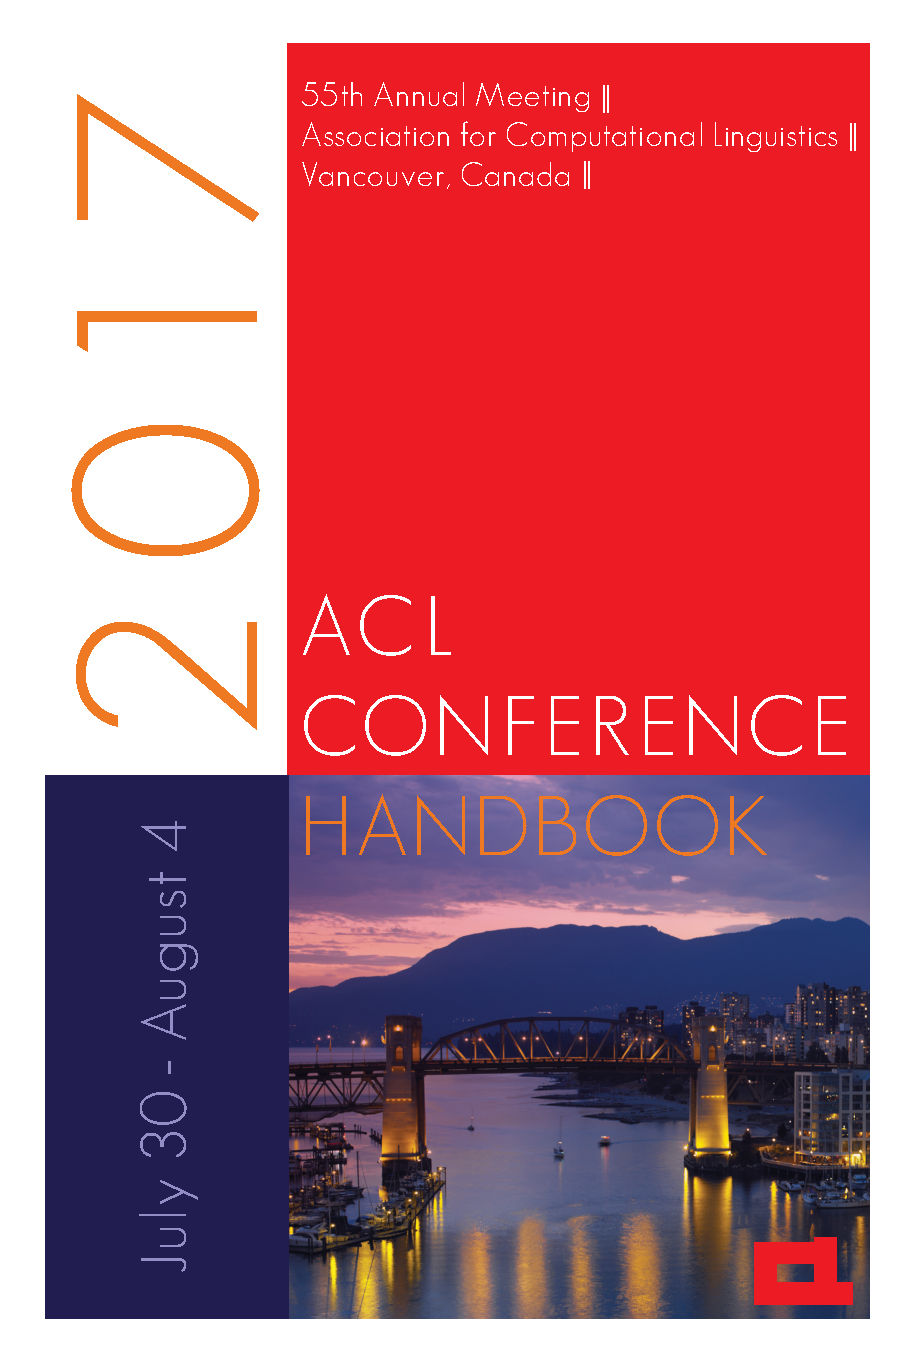
\includepdf[pages={1}]{content/fmatter/cover2.pdf}

\thispagestyle{empty}
\vspace*{6in}
\noindent\emph{Cover design by Sharan Freundschuh Atak}\\\index{Atak, Sharan Freundschuh}
\noindent\emph{Handbook assembled by Christian Federmann (in memoriam Hans-Ulrich Krieger)}\\\index{Federmann, Christian}\index{Krieger, Hans-Ulrich}
\noindent\emph{Printing by Omnipress of Madison, Wisconsin}

\newpage
\cleardoublepage
\fancyfoot[C]{\thepage}
\frontmatter

%% TOC %%%%%%%%%%%%%%%%%%%%%%%%%%%%%%%%%%%%%%%%%%%%%%%%%%%%%%%%%%
\addcontentsline{toc}{chapter}{Table of Contents}
\setcounter{tocdepth}{2}
\tableofcontents
\mainmatter
\pagestyle{fancy}

%% PREFACE %%%%%%%%%%%%%%%%%%%%%%%%%%%%%%%%%%%%%%%%%%%%%%%%%%%%%%
\chapter{Conference Information}

\vspace{2em}

\section{Message from the General Chair}\vspace{2em}
\setheaders%
    {Message from the General Chair}%
    {Message from the General Chair}
\thispagestyle{emptyheader}

\setlength{\parskip}{1ex}


Welcome to ACL 2017 on Vancouver!  We hope you enjoy the conference and your
stay in Canada.    This is the 55th annual meeting of the Association for Computational Linguistics.  We are anticipating one of the largest ACL conferences ever.  We had a record number of papers submitted to the conference, and a record number of industry partners joining us as sponsors of the conference.   We are on track to be one of the best attended ACL conferences to date.   I hope that this year's conference is intellectually stimulating and that you take home many new ideas and techniques that will help extend your own research.

Each year, the ACL conference is organized by a dedicated team of volunteers.  Please thank this year's organizers for their service to the community when you see them at the conference.  Without these people, this conference would not happen:  Regina Barzilay and Min-Yen Kan (Program Co-Chairs),
Priscilla Rasmussen and Anoop Sarkar (Local Organizing Committee),
Wei Xu and  Jonathan Berant (Workshop Chairs),
Maja Popovi\'c and Jordan Boyd-Graber (Tutorial Chairs)
Wei Lu, Sameer Singh and Margaret Mitchell (Publication Chairs),
Heng Ji and Mohit Bansal (Demonstration Chairs),
Spandana Gella, Allyson Ettinger, and Matthieu Labeau (Student Research Workshop Organizers),
Cecilia Ovesdotter Alm, Mark Dredze, and Marine Carpuat (Faculty Advisors to the Student Research Workshop),
Charley Chan  (Publicity Chair),
Christian Federmann (Conference Handbook Chair), 
Maryam Siahbani (Student Volunteer Coordinator), 
and 
Nitin Madnani (Webmaster and Appmaster).

The organizers have been working for more than a year to put together the conference.  Far more than a year in advance, the  ACL 2017 Coordinating Committee helped to select the venue and to pick the General Chair and the Program Co-Chairs.  This consisted of members from  NAACL and ACL executive boards. Representing NAACL we had Hal Daum\'e III,  Michael White, Joel Tetreault,  and Emily Bender.  Representing ACL we had  Pushpak Bhattacharyya, Dragomir Radev,   Graeme Hirst, Yejin Choi, and Priscilla Rasmussen.  I would like to extend a personal thanks to Graeme and Priscilla who often serve as the ACL�s institutional memory, and who have helped fill in many details along the way.

I would like to extend a special thanks to our Program Co-Chairs, Regina Barzilay and Min-Yen Kan.  They documented their work creating the program by running a blog.  They used their blog as a platform for engaging the ACL community in many of the decision making processes including soliciting suggestions for the conference�s area chairs and invited speakers. They hosted discussions with Marti Hearst and Joakim Nivre about the value of publishing pre-prints of submitted paper on arXiv and how they relate to double blind reviewing.  They even invited several prominent members of our community to provide last-minute writing advice.  If you weren�t following the blog in the lead-up to the conference, I highly recommend taking a look through it now.  You can find it linked from the ACL 2017 web page.


This year's program looks like it will be excellent!  We owe a huge thank you
to Regina Barzilay and Min-Yen Kan.  They selected this
year's papers from 1,318 submissions with the help of 44 area chairs and more
than 1,200 reviewers. Thanks to Regina, Min, the area chairs, the reviewers
and the authors. Beyond the papers, we have talks by luminaries in the field
of NLP, including ACL President Joakim Nivre, invited speakers Mirella 
Lapata and Noah Smith, and the recipient of this year's Lifetime Achievement
Award.  We also have an excellent set of workshops and tutorials. 
On the tutorial day, there will also be a special workshop on Women and Underrepresented Minorities in Natural Language Processing.    Thank you to
our workshop organizers and tutorial presenters.

This year we are trying to make ACL more family friendly. We are offering
on-site subsidized childcare for the first time ever, plus a space for nursing
or pumping mothers. Our social event is at the aquarium, which promises to be
a family friendly venue. We hope you bring your loved ones with you.


I would like to thank our many sponsors for their generous contributions.  
Our platinum sponsors are 
Alibaba, 
Amazon, 
Apple, 
Baidu, 
Bloomberg, 
Facebook, 
Google, 
Samsung and 
Tencent.  
Our gold sponsors are 
eBay, 
Elsevier, 
IBM Research, 
KPMG, 
Maluuba, 
Microsoft, 
Naver Line, 
NEC,
Recruit Institute of Technology, and 
SAP.  
Our silver sponsors are 
Adobe,
Bosch,
CVTE,
Duolingo,
Huawei,
Nuance,
Oracle, and
Sogou.
Our bronze sponsors are 
Grammarly, 
Toutiao, and 
Yandex.  
Our supporters include 
Newsela 
and four professional master�s degree programs from 
Brandeis, 
Columbia, 
NYU and 
the University of Washington.  
We would like to acknowledge the generous support of the National Science Foundation which has awarded a \$15,000 grant to the ACL Student Research Workshop.
Finally, NVIDIA donated several Titan X GPU cards for us to raffle off during the conference. 

Lastly, I would like to thank everyone else who helped to make this conference a success.  Thank you to our area chairs, our army of reviewers, our workshop organizers, our tutorial presenters, our invited speakers, and our authors.  Best regards to all of you.

Enjoy the conference! I hope that you learn something new that inspires you to
push your own research to new heights.  
Welcome to ACL 2017!  

\vskip 0.5in
\noindent Best Regards,\\
Chris Callison-Burch\\
ACL 2017 General Chair

\index{Callison-Burch, Chris}

%%%
% General Chair remarks from ACL proceedings -- use these?
%%%

%Welcome to ACL 2017 in Vancouver, Canada!  This is the 55th annual meeting of the Association for Computational Linguistics.  A tremendous amount of knowledge has been presented at more than half a century's worth of our conferences.  
%% Min: sounds too negative?
%Hopefully, some of it is still relevant now that deep learning has solved language.   We are anticipating one of the largest ACL conferences ever.  We had a record number of papers submitted to the conference, and a record number of industry partners joining us a sponsors of the conference.   We are on track to be one of the best attended ACL conferences to date.   I hope that this year's conference is intellectually stimulating and that you take home many new ideas and techniques that will help extend your own research.

%Each year, the ACL conference is organized by a dedicated team of volunteers.  Please thank this year's organizers for their service to the community when you see them at the conference.  Without these people, this conference would not happen:  Regina Barzilay and Min-Yen Kan (Program Co-Chairs),
%Priscilla Rasmussen and Anoop Sarkar (Local Organizing Committee),
%Wei Xu and  Jonathan Berant (Workshop Chairs),
%Maja Popovi\'c and Jordan Boyd-Graber (Tutorial Chairs)
%Wei Lu, Sameer Singh and Margaret Mitchell (Publication Chairs),
%Heng Ji and Mohit Bansal (Demonstration Chairs),
%Spandana Gella, Allyson Ettinger, and Matthieu Labeau (Student Research Workshop Organizers),
%Cecilia Ovesdotter Alm, Mark Dredze, and Marine Carpuat (Faculty Advisors to the Student Research Workshop),
%Charley Chan  (Publicity Chair),
%Christian Federmann (Conference Handbook Chair), 
%Maryam Siahbani (Student Volunteer Coordinator), 
%and 
%Nitin Madnani (Webmaster and Appmaster).

%The organizers have been working for more than a year to put together the conference.  Far more than a year in advance, the  ACL 2017 Coordinating Committee helped to select the venue and to pick the General Chair and the Program Co-Chairs.  This consisted of members from  NAACL and ACL executive boards. Representing NAACL we had Hal Daum\'e III,  Michael White, Joel Tetreault,  and Emily Bender.  Representing ACL we had  Pushpak Bhattacharyya, Dragomir Radev,   Graeme Hirst, Yejin Choi, and Priscilla Rasmussen.  I would like to extend a personal thanks to Graeme and Priscilla who often serve as the ACL’s institutional memory, and who have helped fill in many details along the way.

%I would like to extend a special thanks to our Program Co-Chairs, Regina Barzilay and Min-Yen Kan.  They documented their work creating the program by running a blog.  They used their blog as a platform for engaging the ACL community in many of the decision making processes including soliciting suggestions for the conference’s area chairs and invited speakers.
%% Min: ArXiv => 
%arXiv  They hosted discussions with Marti Hearst and Joakim Nivre about the value of publishing pre-prints of submitted paper on arXiv and how they relate to double blind reviewing.  They even invited several prominent members of our community to provide last-minute writing advice.  If you weren’t following the blog in the lead-up to the conference, I highly recommend taking a look through it now.  You can find it linked from the ACL 2017 web page.

%This year’s conference features two outreach activities that I would like to highlight.  First, on Sunday, July 30, 2017, there will be a workshop on Women and Underrepresented Minorities in Natural Language Processing organized by Libby Barak, Isabelle Augenstein, Chlo\'e Braud, He He,  and Margaret Mitchell.  
%% Min: overrepresented amounts of  underrepresentedness.
%The goals of the workshop are to increase awareness of the work women and underrepresented groups do, support women and underrepresented groups in continuing to pursue their research, and  motivate long-term resourcesfor underrepresented groups within ACL.
%Second, for the first time ever, ACL is offering subsidized on-site childcare at the conference hotel.  The goal of this is to allow ACL participants with children to more readily be able to attend the conference. Since childcare duties often fall disproportionately on women, our hope is that by having professional childcare on-site that we will allow more women to participate, and therefore to help promote their careers.  My hope is that the childcare will be successful, and continued in future conferences. 

%I would like to thank our many sponsors for their generous contributions.  
%Our platinum sponsors are 
%Alibaba, 
%Amazon, 
%Apple, 
%Baidu, 
%Bloomberg, 
%Facebook, 
%Google, 
%Samsung and 
%Tencent.  
%Our gold sponsors are 
%eBay, 
%Elsevier, 
%IBM Research, 
%KPMG, 
%Maluuba, 
%Microsoft, 
%Naver Line, 
%Recruit Institute of Technology, and 
%SAP.  
%Our silver sponsors are 
%Adobe,
%Bosch,
%CVTE,
%% Min: I thought this is capitalized from their website? Duolingo?
%duolingo,
%Huawei,
%Nuance,
%Oracle, and
%Sogou.
%Our bronze sponsors are 
%% Min: I thought this is capitalized from their website? Grammarly?
%grammarly, 
%Toutiao, and 
%Yandex.  
%Our supporters include 
%Newsela 
%and four professional master’s degree programs from 
%% Min: spell out? Brandeis University (since you have UoW)?
%Brandeis, 
%Columbia, 
%% Min: Spell out?
%NYU and 
%the University of Washington.  
%We would like to acknowledge the generous support of the National Science Foundation which has awarded a \$15,000 grant to the ACL Student Research Workshop.
%Finally, NVIDIA donated several Titan X GPU cards for us to raffle off during the conference. 

%Lastly, I would like to thank everyone else who helped to make this conference a success.  Thank you to our area chairs, our army of reviewers, our workshop organizers, our tutorial presenters, our invited speakers, and our authors.  Best regards to all of you.

%Welcome to ACL 2017!

%Chris Callison-Burch \\General Chair

\clearpage
\section{Message from the Program Committee Co-Chairs}
\setheaders%
    {Message from the Program Committee Co-Chairs}%
    {Message from the Program Committee Co-Chairs}
\thispagestyle{emptyheader}
%\renewcommand{\large}{\fontsize{9}{11}\selectfont}
% that's a hack to make this part nicely fill the pages

\setlength{\parskip}{.7ex}
%\setlength{\parindent}{0pt}

Welcome to the 55th Annual Meeting of the Association for
Computational Linguistics! This year, ACL received 751 long paper
submissions and 567 short paper submissions\footnote{These numbers
  exclude papers that were not reviewed due to formatting, anonymity,
  or double submission violations or that were withdrawn prior to
  review, which was unfortunately a substantial number.}. Of the long
papers, 195 were accepted for presentation at ACL — 117 as oral
presentations and 78 as poster presentations (25\% acceptance rate).
107 short papers were accepted — 34 as oral and 73 as poster
presentations (acceptance rate of 18\%). In addition, ACL will also
feature 21 presentations of papers accepted in the {\it Transactions
  of the Association for Computational Linguistics} (TACL). Including
the student research workshop and software demonstrations, the ACL
program swells to a massive total of 367 paper presentations on the
scientific program, representing the largest ACL program to date.

% Min: invited speakers
ACL 2017 will have two distinguished invited speakers: Noah A. Smith
(Associate Professor of Computer Science and Engineering at the
University of Washington) and Mirella Lapata (Professor in the School
of Informatics at the University of Edinburgh).  Both are
well-renowned for their contributions to the field of computational
linguistics and are excellent orators.  We are honored that they have
accepted our invitation to address the membership at this exciting
juncture in our field's history, addressing key issues in
representation learning and multimodal machine translation.

% Min: new innovations
To manage the tremendous growth of our field, we introduced some
changes to the conference. With the rotation of the annual meeting to
the Americas, we anticipated a heavy load of submissions and early on
we decided to have both the long and short paper deadlines merged to
reduce reviewing load and to force authors to take a stand on their
submissions' format.  The joint deadline allowed us to only load our
reviewers once, and also enabled us to have an extended period for
more lengthy dialogue among authors, reviewers and area chairs.  

In addition, oral presentations were shortened to fourteen (twelve)
minutes for long (short) papers, plus time for questions.  While this
places a greater demand on speakers to be concise, we believe it is
worth the effort, allowing far more work to be presented orally. We
also took advantage of the many halls available and expanded the
number of parallel talks to five during most of the conference
sessions.

In keeping with changes introduced in the ACL community from last
year, we continued the practice of recognizing outstanding papers at
ACL. The 22 outstanding papers (15 long, 7 short, 1.6\% of
submissions) represent a broad spectrum of exciting contributions and
have been specially placed on the final day of the main conference
where the program is focused into two parallel sessions of these
outstanding contributions. From these, a best paper and a best short
paper those will be announced in the awards session on Wednesday
afternoon.

%% Following other recent ACL conferences, submissions were reviewed
%% under different categories and using different review forms for
%% empirical/data-driven, theoretical, applications/tools,
%% resources/evaluation, and survey papers. We introduced special fields
%% in the paper submission form for authors to explicitly note the
%% release of open-source implementations to enable reproducibility, and
%% to note freely available datasets.  We also allowed authors to submit
%% appendices of arbitrary length for details that would enable
%% replication; reviewers were not expected to read this material.

%% Another innovation we explored during the review period was the
%% scheduling of short paper review before long paper review. While this
%% was planned to make the entire review period more compact (fitting
%% between the constraints of NAACL 2016 and EMNLP 2016 at either end),
%% we found that reviewing short papers first eliminated many of the
%% surprises for the long paper review process.

%% We sought to follow recently-evolved best practices in planning the
%% poster sessions, so that the many high-quality works presented in that
%% format will be visible and authors and attendees benefit from the
%% interactions during the two poster sessions.

Chris has already mentioned our introduction of the chairs'
blog\footnote{\url{https://chairs-blog.acl2017.org/}}, where we strove
to make the selection process of the internal workings of the
scientific committee more transparent.  We have publicly documented
our calls for area chairs, reviewers and accepted papers selection
process.  Via the blog, we communicated several innovations in the
conference organization workflow, of which we would call attention to
two key ones here.

In the review process, we pioneered the use of the Toronto Paper
Matching System, a topic model based approach to the assignment of
reviewers to papers.  We hope this decision will spur other program
chairs to adopt the system, as increased coverage will better the
reviewer/submission matching process, ultimately leading to a higher
quality program.

For posterity, we also introduced the usage of hyperlinks in the
bibliography reference sections of papers, and have worked with the
ACL Anthology to ensure that digital object identifiers (DOIs) appear
in the footer of each paper.  These steps will help broaden the
long-term impact of the work that our community has on the scientific
world at large.

There are many individuals we wish to thank for their contributions
to ACL 2017, some multiple times:

\begin{itemize}
\item The 61 area chairs who volunteered for our extra duty. They
  recruited reviewers, led discussions on each paper, replied to
  authors' direct comments to them and carefully assessed each
  submission.  Their input was instrumental in guiding the final
  decisions on papers and selecting the outstanding papers.
%
% Mausam, Omri Abend, Eugene Agichtein, Ron Artstein, Alexandra Balahur,
% Mohit Bansal, Chia-Hui Chang, Grzegorz Chrupała, Mona Diab, Jason
% Eisner, Manaal Faruqui, Raquel Fernandez, Karën Fort, Amir Globerson,
% Hannaneh Hajishirzi, Chiori Hori, Tommi Jaakkola, Yangfeng Ji, Jing
% Jiang, Sarvnaz Karimi, Anna Korhonen, Zornitsa Kozareva, Lun-Wei Ku,
% Nate Kushman, Chia-ying Lee, Oliver Lemon, Roger Levy, Sujian Li,
% Wenjie Li, Kang Liu, Tie-Yan Liu, Yang Liu, Zhiyuan Liu, Minh-Thang
% Luong, Saif M Mohammad, Alexander M Rush, Haitao Mi, Alessandro
% Moschitti, Smaranda Muresan, Preslav Nakov, Graham Neubig, Aurélie
% Névéol, Shimei Pan, Michael Piotrowski, Emily Pitler, Barbara Plank,
% Sujith Ravi, Verena Rieser, Sophie Rosset, Mehroosh Sadrzadeh, Hinrich
% Schütze, Anders Søgaard, Karin Verspoor, Aline Villavicencio, Svitlana
% Volkova, Bonnie Webber, Deyi Xiong, William Yang Wang, Wajdi
% Zaghouani, Yue Zhang and Hai Zhao.

\item Our full program committee of BUG hard-working individuals who
  reviewed the conference’s 1,318 submissions (including secondary
  reviewers).
\item TACL editors-in-chief Mark Johnson, Lillian Lee, and Kristina
  Toutanova, for coordinating with us on TACL presentations at ACL.
\item Noah Smith and Katrin Erk, program co-chairs of ACL 2016 and Ani
  Nenkova and Owen Rambow, program co-chairs of NAACL 2016, who we
  consulted several times on short order for help and advice.
\item Wei Lu and Sameer Singh, our well-organized publication chairs,
  with direction and oversight from publication chair mentor Meg
  Mitchell.  Also, Christian Federmann who helped with the local
  handbook.
\item The responsive team at Softconf led by Rich Gerber, who worked
  quickly to resolve problems and who strove to integrate the use of
  the Toronto Paper Matching System (TPMS) for our use.
\item Priscilla Rasmussen and Anoop Sarkar and the local organization
  team, especially webmaster Nitin Madnani.
\item Christopher Calliston-Burch, our general chair, who kept us
  coordinated with the rest of the ACL 2017 team and helped us free
  our time to concentrate on the key duty of organizing the scientific
  program.
\item Key-Sun Choi, Jing Jiang, Graham Neubig, Emily Pitler, and
  Bonnie Webber who carefully reviewed papers under consideration for
  best paper recognition.
\item Our senior correspondents for the blog, who contributed guest
  posts and advice for writing and reviewing: Waleed Ammar, Yoav
  Artzi, Tim Baldwin, Marco Baroni, Claire Cardie, Xavier Carreras,
  Hal Daumé, Kevin Duh, Chris Dyer, Marti Hearst, Mirella Lapata,
  Emily M. Bender, Aurélien Max, Kathy McKeown, Ray Mooney, Ani
  Nenkova, Joakim Nivre, Philip Resnik, and Joel Tetreault.  Without
  them, the participation of the community through the productive
  comments, and without you the readership, our blog for disseminating
  information about the decision processes would not have been
  possible and a success.
\end{itemize}

We hope that you enjoy ACL 2017 in Vancouver!

\noindent ACL 2017 program co-chairs\\
Regina Barzilay, Massachusetts Institute of Technology\\
Min-Yen Kan, National University of Singapore


\clearpage%{\thispagestyle{emptyheader}\cleardoublepage}
\setheaders{}{}
\markboth{}{} % clear the right header
\markright{}{} % clear the right header

\section{Organizing Committee}{}

\setlength{\parindent}{0pt}

{\bf General Chair} \\
Chris Callison-Burch, University of Pennsylvania

{\bf Program Committee Co-chairs} \\
Regina Barzilay, Massachusetts Institute of Technology\\
Min-Yen Kan, National University of Singapore

{\bf Local Organizing Committee} \\
Priscilla Rasmussen, ACL\\
Anoop Sarkar, Simon Fraser University

{\bf Workshop Co-chairs} \\
Wei Xu, Ohio State University \\
Jonathan Berant, Tel Aviv University

{\bf Tutorial Co-chairs} \\
Maja Popovi\'{c}, Humboldt-Universität zu Berlin \\
Jordan Boyd-Graber, University of Colorado, Boulder

{\bf Publication Co-chairs} \\
Wei Lu, Singapore University of Technology and Design \\
Sameer Singh, University of California, Irvine \\
Margaret Mitchell, Google (Advisory)

{\bf Demonstration Chairs} \\
Heng Ji, Rensselaer Polytechnic Institute \\
Mohit Bansal, University of North Carolina, Chapel Hill

{\bf Student Research Workshop Organizers} \\
\hspace*{0.2in} Spandana Gella, University of Edinburgh \\
\hspace*{0.2in} Allyson Ettinger, University of Maryland, College Park \\
\hspace*{0.2in} Matthieu Labeau, Laboratoire d’Informatique pour la Mécanique et les Sciences de l’Ingénieur (LIMSI) \\

{\bf Faculty Advisors to the Student Research Workshop} \\
\hspace*{0.2in} Cecilia Ovesdotter Alm, Rochester Institute of Technology \\
\hspace*{0.2in} Mark Dredze, Johns Hopkins University \\
\hspace*{0.2in} Marine Carpuat, University of Maryland, College Park

{\bf Publicity Chair} \\
Charley Chan, Bloomberg

{\bf Conference Handbook Chair} \\
Christian Federmann, Microsoft

{\bf Student Volunteer Coordinator} \\
Maryam Siahbani, University of the Fraser Valley

{\bf Reviewing Coordinators} \\
Mark Dredze, Johns Hopkins University \\
Jiang Guo, Harbin Institute of Technology

{\bf Webmaster and Appmaster} \\
Nitin Madnani, Educational Testing Service

%%%%%%%%%%%%%%%%%%%%%%%%%%%%%%%%%%%%%%%%%%%%%%%%%%%%%%%%%%%%%%%%%%%%%%%%

\clearpage
\section{Program Committee}
\setlength{\parindent}{0pt}

\vspace*{0.5cm}

{\bf Program Committee Co-chairs} \\
Regina Barzilay, Massachusetts Institute of Technology \\
Min-Yen Kan, National University of Singapore

{\bf Area Chairs} \\
\emph{Dialogue and Interactive Systems} \\
\hspace*{0.2in} Ron Artstein \\
\hspace*{0.2in} Raquel Fernandez \\
\hspace*{0.2in} Oliver Lemon

\emph{Discourse and Pragmatics} \\
\hspace*{0.2in} Yangfeng Ji \\
\hspace*{0.2in} Sujian Li \\
\hspace*{0.2in} Bonnie Webber
 
\emph{Summarization and Generation} \\
\hspace*{0.2in} Wenjie Li \\
\hspace*{0.2in} Alexander M Rush \\
\hspace*{0.2in} Verena Rieser

\emph{Information Extraction and NLP Applications} \\
\hspace*{0.2in} Mausam \\
\hspace*{0.2in} Eugene Agichtein \\
\hspace*{0.2in} Chia-Hui Chang \\
\hspace*{0.2in} Jing Jiang \\
\hspace*{0.2in} Sarvnaz Karimi \\
\hspace*{0.2in} Zornitsa Kozareva \\
\hspace*{0.2in} Kang Liu \\
\hspace*{0.2in} Tie-Yan Liu \\
\hspace*{0.2in} Alessandro Moschitti \\
\hspace*{0.2in} Smaranda Muresan

\emph{Multilingual} \\
\hspace*{0.2in} Omri Abend \\
\hspace*{0.2in} Mona Diab

\emph{Sentiment Analysis and Opinion Mining} \\
\hspace*{0.2in} Alexandra Balahur \\
\hspace*{0.2in} Lun-Wei Ku \\
\hspace*{0.2in} Saif M Mohammad

\emph{Vision, Robotics and Grounding} \\
\hspace*{0.2in} Mohit Bansal \\
\hspace*{0.2in} Nate Kushman

\emph{Machine Learning} \\
\hspace*{0.2in} Grzegorz Chrupała \\
\hspace*{0.2in} Amir Globerson \\
\hspace*{0.2in} Tommi Jaakkola \\
\hspace*{0.2in} Sujith Ravi \\
\hspace*{0.2in} William Yang Wang

\emph{Phonology, Morphology and Word Segmentation} \\
\hspace*{0.2in} Jason Eisner \\
\hspace*{0.2in} Hinrich Schütze

\emph{Semantics} \\
\hspace*{0.2in} Manaal Faruqui \\
\hspace*{0.2in} Hannaneh Hajishirzi \\
\hspace*{0.2in} Anna Korhonen \\
\hspace*{0.2in} Preslav Nakov \\
\hspace*{0.2in} Mehroosh Sadrzadeh \\
\hspace*{0.2in} Aline Villavicencio

\emph{Multidisciplinary} \\
\hspace*{0.2in} Karën Fort \\
\hspace*{0.2in} Michael Piotrowski

\emph{Speech} \\
\hspace*{0.2in} Chiori Hori \\
\hspace*{0.2in} Chia-ying Lee

\emph{Discourse and Pragmatics} \\
\hspace*{0.2in} Yangfeng Ji \\
\hspace*{0.2in} Sujian Li \\
\hspace*{0.2in} Bonnie Webber

\emph{Cognitive Modeling and Psycholinguistics} \\
\hspace*{0.2in} Roger Levy \\
\hspace*{0.2in} Anders Søgaard

\emph{Machine Translation} \\
\hspace*{0.2in} Yang Liu \\
\hspace*{0.2in} Minh-Thang Luong \\
\hspace*{0.2in} Haitao Mi \\
\hspace*{0.2in} Graham Neubig \\
\hspace*{0.2in} Deyi Xiong

\emph{Social Media} \\
\hspace*{0.2in} Zhiyuan Liu \\
\hspace*{0.2in} Shimei Pan \\
\hspace*{0.2in} Svitlana Volkova

\emph{Biomedical} \\
\hspace*{0.2in} Aurélie Névéol \\
\hspace*{0.2in} Karin Verspoor

\emph{Tagging, Chunking, Syntax and Parsing} \\
\hspace*{0.2in} Emily Pitler \\
\hspace*{0.2in} Barbara Plank \\
\hspace*{0.2in} Yue Zhang \\
\hspace*{0.2in} Hai Zhao

\emph{Resources and Evaluation} \\
\hspace*{0.2in} Sophie Rosset \\
\hspace*{0.2in} Wajdi Zaghouani


\clearpage%{\thispagestyle{emptyheader}\cleardoublepage}
\setheaders{}{}

\setheaders{}{}
\section{Meal Info}{}

The following meals are provided as part of your registration fee:

\begin{itemize}
\item A full buffet breakfast will be provided each day in the \BreakfastLoc
\item Mid-Morning breaks include coffee and tea in the \BreakLoc
\item Mid-Afternoon breaks include coffee, tea, soda, water, and
  snacks in the \BreakLoc
\item A full dinner buffer is provided during the poster sessions on
  Monday and Tuesday evenings in the \PosterSessionLoc
\end{itemize}

\clearpage

%% TUTORIALS %%%%%%%%%%%%%%%%%%%%%%%%%%%%%%%%%%%%%%%%%%%%%%%%%%%%
\setdaydateyear{Sunday}{July 30}{2017}
% This file is just done manually

\chapter{Tutorials: \daydate}
\thispagestyle{emptyheader}
\setheaders{Tutorials}{\daydateyear}
\setlength{\parindent}{0in}
\setlength{\parskip}{2ex}
\renewcommand{\baselinestretch}{0.87}

\newcommand{\tutorialmorningtime}{9:00--12:30}
\newcommand{\tutorialafternoontime}{14:00--17:30}

\section*{Overview}
\renewcommand{\arraystretch}{1.2}
\begin{SingleTrackSchedule}
  7:30 & -- & 18:00 &
  {\bfseries Registration} \hfill\emph{\RegistrationLoc}
  \\
  7:30 & -- & 9:00 &
  {\bfseries Breakfast} \hfill\emph{\BreakfastLoc}
  \\
  9:00 & -- & 12:30 &
  {\bfseries Morning Tutorials} \hfill
  \\
  & & & \papertitle{tutorial-001}\hfill\emph{\TutLocA}\newline
  \tutorialauthors{tutorial-001} \\
  \\
  & & & \papertitle{tutorial-002}\hfill\emph{\TutLocB}\newline
  \tutorialauthors{tutorial-002} \\
  \\
  & & & \papertitle{tutorial-003}\hfill\emph{\TutLocC}\newline
  \tutorialauthors{tutorial-003} \\
  \\
  10:30 & -- & 11:00 &
  {\bfseries Coffee break}
  \\
  12:30 & -- & 14:00 &
  {\bfseries Lunch break}
  \\
  14:00 & -- & 17:30 &
  {\bfseries Afternoon Tutorials} \hfill
  \\
  & & & \papertitle{tutorial-004}\hfill\emph{\TutLocD}\newline
  \tutorialauthors{tutorial-004} \\
  \\
  & & & \papertitle{tutorial-005}\hfill\emph{\TutLocE}\newline
  \tutorialauthors{tutorial-005} \\
  \\
  & & & \papertitle{tutorial-006}\hfill\emph{\TutLocF}\newline
  \tutorialauthors{tutorial-006} \\
  \\
  15:30 & -- & 16:00 &
  {\bfseries Coffee break}
  \\
  18:00 & -- & 21:00 &
  {\bfseries Welcome Reception} \hfill \emph{\WelcomeReceptionLoc}
  \\
\end{SingleTrackSchedule}

\clearpage\section{Message from the Tutorial Co-Chairs}\vspace{2em}
\setheaders%
    {Message from the Tutorial Co-Chairs}%
    {Message from the Tutorial Co-Chairs}
\thispagestyle{emptyheader}

\setlength{\parskip}{1ex}

This section contains the abstracts of the ACL 2017 tutorials. This year we had a joint call-for-tutorials, coordinated with the EACL and EMNLP co-chairs (6 co-chairs in total). We received 26 submissions for the joint ACL/EACL/EMNLP call, and it was a difficult task to make a final selection. The six co-chairs applied the following criteria for evaluation: relevance to ACL community, quality of proposal, quality of instructor, estimate of attendance, relevance of area. The tutorials were then assigned to venues trying to respect proposers' preferences and to balance topics across venues. Nine tutorials had ACL as the preferred conference, from which one was rejected, two were redirected to EMNLP and the rest (six of them) was accepted. All six are organised as half-day tutorials.

We are very grateful to Alex Klementiev and Lucia Specia (EACL tutorial chairs), Nathan Schneider and Alexandra Birch (EMNLP tutorial chairs), Priscilla Rasmussen and Anoop Sarkar (local chairs), Wei Lu, Sameer Singh and Margaret Mitchell (publication chairs), Min-Yen Kan and Regina Barzilay (program co-chairs) and of course Chris Callison-Burch (general chair) for various kinds of help, advice and assistance offered during the process of putting the tutorial programme and materials together. Most importantly, we would like to thank the tutorial presenters for the time and effort in preparing and presenting the tutorials.

We hope you will enjoy the tutorials!

\vskip 0.5in
\noindent ACL 2017 Tutorial Chairs\\
\noindent Maja Popović, Humboldt-Universität zu Berlin\\
\index{Popović, Maja}
\noindent Jordan Boyd-Graber, University of Colorado, Boulder\\
\index{Boyd-Graber, Jordan}


\setheaders{Tutorials}{\daydateyear}
\clearpage\begin{bio}
  {\bfseries Hoifung Poon} is a Researcher at Microsoft Research Redmond. His research interests lie in advancing machine learning and natural language processing (NLP) to help automate discovery and decision support in precision medicine. He received his Ph.D. in computer science \& engineering at the University of Washington. His past work has been recognized with Best Paper Awards from premier NLP and machine learning venues such as NAACL-09 (unsupervised morphological segmentation), EMNLP-09 (unsupervised semantic parsing), and UAI-11 (sum-product networks).

  {\bfseries Chris Quirk} is a Principal Researcher at Microsoft Research Redmond. Since joining Microsoft Research in 2001, his research has focused on effective computational systems for aiding human communication, understanding, and task completion. His primary focus is in machine translation, building practical and widely-used system implementations and authoring a number of influential papers. He has also worked in paraphrase, information extraction, and most recently biological applications of natural language processing and machine learning. He has served on numerous program committees, acted Area Chair (ACL 2010, EMNLP 2012), and is currently an action editor of the TACL journal.

  {\bfseries Kristina Toutanova} is a Staff Research Scientist at Google Research Seattle and affiliate faculty member at the University of Washington. In 2005, she obtained her Ph.D. from the Computer Science Department at Stanford University, where she was advised by Christopher Manning. She focuses on modeling the structure of natural language using machine learning, in the areas of semantic parsing, knowledge extraction, information retrieval, and text-to-text generation. She has coauthored more than 50 publications at refereed conferences and journals, including four papers that have won awards at conferences (EMNLP, NAACL, CoNLL, ECML). She served as a program co-chair for CoNLL 2008 and ACL 2014 and is currently serving as a co-editor-in-chief of the TACL journal.

  {\bfseries Wen-tau Yih} is a Senior Researcher at Microsoft Research Redmond. His research interests include natural language processing, machine learning and information retrieval. Yih received his Ph.D. in computer science at the University of Illinois at Urbana-Champaign. His work on joint inference using integer linear programming (ILP) helped the UIUC team win the CoNLL-05 shared task on semantic role labeling, and the approach has been widely adopted in the NLP community since then. After joining MSR in 2005, he has worked on email spam filtering, keyword extraction and search & ad relevance. His recent work focuses on continuous semantic representations using neural networks and matrix/tensor decomposition methods, with applications in lexical semantics, knowledge base embedding and question answering. Yih received the best paper award from CoNLL-2011, an outstanding paper award from ACL-2015 and has served as area chairs (HLT-NAACL-12, ACL-14, EMNLP16,17), program co-chairs (CEAS-09, CoNLL-14) and action/associated editors (TACL, JAIR) in recent years.

\end{bio}

\begin{tutorial}
  {Natural Language Processing for Precision Medicine}
  {tutorial-final-001}
  {\daydateyear, \tutorialmorningtime}
  {\TutLocA}

We will introduce precision medicine and showcase the vast opportunities for NLP in this burgeoning field with great societal impact. We will review pressing NLP problems, state-of-the art methods, and important applications, as well as datasets, medical resources, and practical issues. The tutorial will provide an accessible overview of biomedicine, and does not presume knowledge in biology or healthcare. The ultimate goal is to reduce the entry barrier for NLP researchers to contribute to this exciting domain.
\end{tutorial}

\clearpage\begin{bio}
  {\bfseries Louis-Philippe Morency} (\url{https://www.cs. cmu.edu/~morency/}) is Assistant Professor in the Language Technology Institute at the Carnegie Mellon University where he leads the Multimodal Communication and Machine Learning Laboratory (MultiComp Lab). He received his Ph.D. and Master degrees from MIT Computer Science and Artificial Intelligence Laboratory. In 2008, Dr. Morency was selected as one of ”AI’s 10 to Watch” by IEEE Intelligent Systems. He has received 7 best paper awards in multiple ACMand IEEE-sponsored conferences for his work on context-based gesture recognition, multimodal probabilistic fusion and computational models of human communication dynamics. Dr. Morency was General Chair for the International Conference on Multimodal Interaction (ICMI 2012) and the NIPS 2010 workshop on Modeling Human Communication Dynamics. He was Program Chair for ICMI 2011, 2014 and 2016, as well as the Tenth International Conference on Creating, Connecting and Collaborating through Computing in January 2012.
  \index{Morency, Louis-Philippe}
 
  {\bfseries Tadas Baltrusaitis} (\url{http://www.cl.cam. ac.uk/~tb346/}) is a post-doctoral associate at the Language Technologies Institute, Carnegie Mellon University. Before this, he was a postdoctoral research at the University of Cambridge, where he also received his PhD degree in 2014. His primary research interests lie in the automatic understanding of non-verbal human behaviour, computer vision, and multimodal machine learning. His papers have won a number of awards for his work on non-verbal human behavior analysis, including ICMI 2014 best student paper award, and ETRA 2016 emerging investigator award. He is also a winner of several challenges in computer vision and multi-modal machine learning, including FERA 2015, and AVEC 2011.
  \index{Baltrusaitis, Tadas}
\end{bio}

\begin{tutorial}
  {Multimodal Machine Learning}
  {tutorial-002}
  {\daydateyear, \tutorialmorningtime}
  {\TutLocB}

Multimodal machine learning is a vibrant multi-disciplinary research field which addresses some of the original goals of artificial intelligence by integrating and modeling multiple communicative modalities, including linguistic, acoustic and visual messages. With the initial research on audio-visual speech recognition and more recently with image and video captioning projects, this research field brings some unique challenges for multimodal researchers given the heterogeneity of the data and the contingency often found between modalities.
 
This tutorial builds upon a recent course taught at Carnegie Mellon University during the Spring 2016 semester (CMU course 11-777) and two tutorials presented at CVPR 2016 and ICMI 2016. The present tutorial will review fundamental concepts of machine learning and deep neural networks before describing the five main challenges in multimodal machine learning: (1) multimodal representation learning, (2) translation \& mapping, (3) modality alignment, (4) multimodal fusion and (5) co-learning. The tutorial will also present state-of-the-art algorithms that were recently proposed to solve multimodal applications such as image captioning, video descriptions and visual question-answer. We will also discuss the current and upcoming challenges.
\end{tutorial}

\clearpage\begin{bio}
  {\bfseries Xiaodan Zhu} is an assistant professor of the Department of Electrical and Computer Engineering of Queen’s University, Canada. Before that, he was a Research Officer of the National Research Council Canada. His research interests are in Natural Language Processing and Machine Learning. His recent work has focused on deep learning, semantic composition, sentiment analysis, and natural language inference.

  {\bfseries Edward Grefenstette} is a Staff Research Scientist at DeepMind. His research covers the intersection of Machine Learning, Computer Reasoning, and Natural Language Understanding. Recent publications cover the topics of neural computation, representation learning at the sentence level, recognising textual entailment, and machine reading. 
\end{bio}

\begin{tutorial}
  {Deep Learning for Semantic Composition}
  {tutorial-final-003}
  {\daydateyear, \tutorialmorningtime}
  {\TutLocC}

Learning representation to model the meaning of text has been a core problem in NLP. The last several years have seen extensive interests on distributional approaches, in which text spans of different granularities are encoded as vectors of numerical values. If properly learned, such representation has showed to achieve the state-of-the-art performance on a wide range of NLP problems.
 
In this tutorial, we will cover the fundamentals and the state-of-the-art research on neural network-based modeling for semantic composition, which aims to learn distributed representation for different granularities of text, e.g., phrases, sentences, or even documents, from their sub-component meaning representation, e.g., word embedding.
\end{tutorial}

\clearpage\begin{bio}
  {\bfseries Yun-Nung Chen} is currently an assistant professor at the Department of Computer Science, National Taiwan University. She earned her Ph.D. degree from Carnegie Mellon University, where her research interests focus on spoken dialogue system, language understanding, natural language processing, and multi-modal speech applications. She received the Google Faculty Research Awards 2016, two Student Best Paper Awards from IEEE SLT 2010 and IEEE ASRU 2013, a Student Best Paper Nominee from Interspeech 2012, and the Distinguished Master Thesis Award from ACLCLP. Before joining National Taiwan University, she worked in the Deep Learning Technology Center at Microsoft Research Redmond. More information about her can be found at \url{http://vivianchen.idv.tw}.

  {\bfseries Asli Celikyilmaz} is currently a researcher at the Deep Learning Technology Center at Microsfot Research. Previously, she was a Research Scientist at Microsoft Bing from 2010 until 2016 focusing on deep learning models for scaling natural user interfaces to multiple domains. She has worked as a Postdoc Researcher at the EECS Department of the UC Berkeley from 2008 until 2010. She has worked with researchers at ICSI @ Berkeley during her postdoc research study. She earned her Ph.D. from University of Toronto, Canada in 2008. Asli’s research interests are mainly machine learning and its applications to conversational dialogue systems, mainly natural language understanding and dialogue modeling. In the past she has also focused on research areas including machine intelligence, semantic tagging of natural user utterances of human to machine conversations, text analysis, document summarization, question answering, co-reference resolution, to name a few. Currently she is focusing on reasoning, attention, memory networks as well as multi-task and transfer learning for conversational dialogue systems. She has been serving as area chair, co-organizer of numerous NLP and speech conferences, such as ACL, NAACL, Interspeech, and IEEE Spoken Language Technologies (SLT). She co-organized a NIPS workshop on Machine Learning for Spoken Language Understanding and Interactions in 2015.

  {\bfseries Dilek Hakkani-Tur} is a research scientist at Google Research. Prior to joining Google, she was a researcher at Microsoft Research (2010-2016), International Computer Science Institute (ICSI, 2006-2010) and AT\&T Labs-Research (20012005). She received her BSc degree from Middle East Technical Univ, in 1994, and MSc and PhD degrees from Bilkent Univ., Department of Computer Engineering, in 1996 and 2000, respectively. Her research interests include natural language and speech processing, spoken dialogue systems, and machine learning for language processing. She has over 50 patents that were granted and co-authored more than 200 papers in natural language and speech processing. She is the recipient of three best paper awards for her work on active learning for dialogue systems, from IEEE Signal Processing Society, ISCA and EURASIP. She was an associate editor of IEEE Transactions on Audio, Speech and Language Processing (20052008), member of the IEEE Speech and Language Technical Committee (2009-2014), area editor for speech and language processing for Elsevier’s Digital Signal Processing Journal and IEEE Signal Processing Letters (2011-2013), and currently serves on ISCA Advisory Council (20152018). She is a fellow of IEEE and ISCA. 
\end{bio}

\begin{tutorial}
  {Deep Learning for Dialogue Systems}
  {tutorial-final-004}
  {\daydateyear, \tutorialafternoontime}
  {\TutLocD}

In the past decade, goal-oriented spoken dialogue systems have been the most prominent component in today's virtual personal assistants. The classic dialogue systems have rather complex and/or modular pipelines. The advance of deep learning technologies has recently risen the applications of neural models to dialogue modeling. However, how to successfully apply deep learning based approaches to a dialogue system is still challenging. Hence, this tutorial is designed to focus on an overview of the dialogue system development while describing most recent research for building dialogue systems and summarizing the challenges, in order to allow researchers to study the potential improvements of the state-of-the-art dialogue systems. The tutorial material is available at \url{http://deepdialogue.miulab.tw}.
\end{tutorial}

\clearpage\begin{bio}
  {\bfseries Valia Kordoni} is a professor at Humboldt-Universität zu Berlin,
  Germany. 

\end{bio}

\begin{tutorial}
  {Beyond Words: Deep Learning for Multi-word Expressions and Collocations}
  {tutorial-final-005}
  {\daydateyear, \tutorialafternoontime}
  {\TutLocE}

Deep learning has recently shown much promise for NLP applications.
Traditionally, in most NLP approaches, documents or sentences are represented
by a sparse bag-of-words representation. There is now a lot of work which goes
beyond this by adopting a distributed representation of words, by constructing
a so-called ``neural embedding'' or vector space representation of each word or
document. The aim of this tutorial is to go beyond the learning of word
vectors and present methods for learning vector representations for Multiword
Expressions and bilingual phrase pairs, all of which are useful for various NLP
applications.

This tutorial aims to provide attendees with a clear notion of the linguistic
and distributional characteristics of Multiword Expressions (MWEs), their
relevance for the intersection of deep learning and natural language
processing, what methods and resources are available to support their use, and
what more could be done in the future. Our target audience are researchers and
practitioners in machine learning, parsing (syntactic and semantic) and
language technology, not necessarily experts in MWEs, who are interested in
tasks that involve or could benefit from considering MWEs as a pervasive
phenomenon in human language and communication.

\end{tutorial}
\clearpage\begin{bio}
  {\bfseries Jennifer Wortman Vaughan} is a researcher at Microsoft Research,
  New York City. She is interested in developing general methods that allow us
  to reason formally about the performance of algorithms with human components
  in the same way that traditional computer science techniques allow us to
  formally reason about algorithms that run on machines alone.

\end{bio}

\begin{tutorial}
  {Making Better Use of the Crowd}
  {tutorial-final-006}
  {\daydateyear, \tutorialafternoontime}
  {\TutLocF}

Over the last decade, crowdsourcing has been used to harness the power of human
computation to solve tasks that are notoriously difficult to solve with
computers alone, such as determining whether or not an image contains a tree,
rating the relevance of a website, or verifying the phone number of a business.
The natural language processing community was early to embrace crowdsourcing as
a tool for quickly and inexpensively obtaining annotated data to train NLP
systems. Once this data is collected, it can be handed off to algorithms that
learn to perform basic NLP tasks such as translation or parsing. Usually this
handoff is where interaction with the crowd ends. The crowd provides the data,
but the ultimate goal is to eventually take humans out of the loop. Are there
better ways to make use of the crowd?

In this tutorial, I will begin with a showcase of innovative uses of
crowdsourcing that go beyond data collection and annotation. I will discuss
applications to natural language processing and machine learning, hybrid
intelligence or “human in the loop” AI systems that leverage the complementary
strengths of humans and machines in order to achieve more than either could
achieve alone, and large scale studies of human behavior online. I will then
spend the majority of the tutorial diving into recent research aimed at
understanding who crowdworkers are, how they behave, and what this should
teach us about best practices for interacting with the crowd.

\end{tutorial}


%% RECEPTION %%%%%%%%%%%%%%%%%%%%%%%%%%%%%%%%%%%%%%%%%%%%%%%%%%%%
\newpage
\addcontentsline{toc}{chapter}{Welcome Reception: \daydate, 18:00}
\clearpage
\section[Welcome Reception]{Welcome Reception}
\setheaders{}{\daydateyear}

\begin{center}

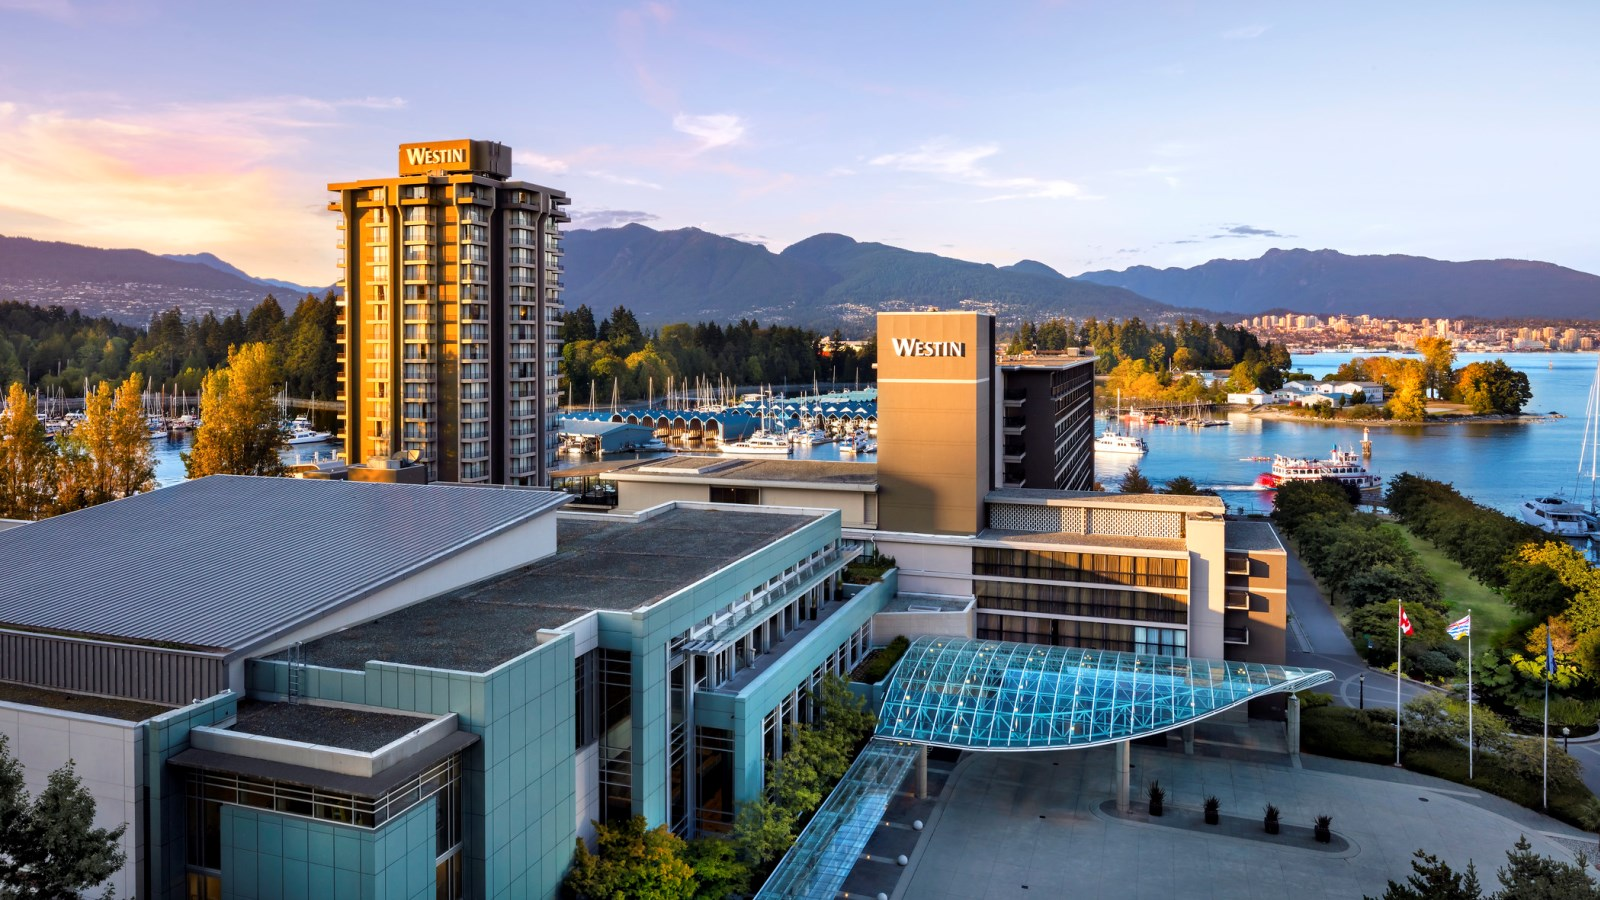
\includegraphics[width=4in]{content/ACL17-westin-bayshore.jpg}

\vspace{2ex}\centerline{\rule{.5\linewidth}{.5pt}}\vspace{2ex}
\setlength{\parskip}{1ex}\setlength{\parindent}{0ex}

\daydateyear, 18:00 -- 21:00 \vspace{1em}\\
Westin Bayshore Hotel (Conference Venue)\\
\WelcomeReceptionLoc\\
\url{http://www.westinbayshore.com/}
\end{center}

\noindent Catch up with your colleagues at the \textbf{Welcome
Reception}! It will be held immediately following the Tutorials
on \daydate at 6:00pm in the Bayshore Grand Ballroom of the Westin
Bayshore Hotel (the conference venue). Refreshments and a light
dinner will be provided, and a cash bar will be available.


%% MAIN CONFERENCE %%%%%%%%%%%%%%%%%%%%%%%%%%%%%%%%%%%%%%%%%%%%%%
\setdaydateyear{Monday}{July 31}{2017}
\chapter{Main Conference: \daydate}
\thispagestyle{emptyheader}
\setheaders{Main Conference}{\daydateyear}

%% Overview page %%%%%%%%%%%%%%%%%%%%%%%%%%%%%%%%%%%%%%%%%%%%%%%%
\section*{Overview}
\renewcommand{\arraystretch}{1.2}
\begin{SingleTrackSchedule}
  7:30 & -- & 9:00 &
  {\bfseries Breakfast} \hfill\emph{\BreakfastLoc}
  \\[-2mm]
  9:00 & -- & 10:00 &
  {\bfseries Plenary Session. Welcome to ACL 2017!} \hfill \emph{\PlenaryLoc}\\
  & & & Presidential Address: Joakim Nivre\\
  \\[-2mm]
  10:00 & -- & 10:30 &
  {\bfseries Coffee break} \hfill \emph{\CoffeeLoc}\\
  \\[-2mm]
  10:30 & -- & 12:00 &
  \begin{tabular}{|p{0.66000000000in}|p{0.66000000000in}|p{0.66000000000in}|p{0.66000000000in}|p{0.66000000000in}|}
    \multicolumn{5}{l}{{\bfseries Session 1}}\\\hline
Information Extraction 1 (NN) & Semantics 1 & Discourse 1 & Machine Translation 1 & Generation 1 \\
\emph{\TrackALoc} & \emph{\TrackBLoc} & \emph{\TrackCLoc} & \emph{\TrackDLoc} & \emph{\TrackELoc} \\
  \hline\end{tabular} \\
  \\[-2mm]
  12:00 & -- & 13:40 &
  {\bfseries Lunch break} \hfill \emph{\LunchLoc}\\
  \\[-2mm]
  13:40 & -- & 15:15 &
  \begin{tabular}{|p{0.66000000000in}|p{0.66000000000in}|p{0.66000000000in}|p{0.66000000000in}|p{0.66000000000in}|}
    \multicolumn{5}{l}{{\bfseries Session 2}}\\\hline
Question Answering 1 & Vision 1 & Syntax 1 & Machine Learning 1 (NN) & Sentiment 1 (NN) \\
\emph{\TrackALoc} & \emph{\TrackBLoc} & \emph{\TrackCLoc} & \emph{\TrackDLoc} & \emph{\TrackELoc} \\
  \hline\end{tabular} \\
  \\[-2mm]
  15:15 & -- & 15:45 &
  {\bfseries Coffee break} \hfill \emph{\CoffeeLoc}\\
  \\[-2mm]
  15:45 & -- & 17:20 &
  \begin{tabular}{|p{0.66000000000in}|p{0.66000000000in}|p{0.66000000000in}|p{0.66000000000in}|p{0.66000000000in}|}
    \multicolumn{5}{l}{{\bfseries Session 3}}\\\hline
Information Extraction 2 / Biomedical 1 & Semantics 2 (NN) & Speech 1 / Dialogue 1 & Multilingual 1 & Phonology 1 \\
\emph{\TrackALoc} & \emph{\TrackBLoc} & \emph{\TrackCLoc} & \emph{\TrackDLoc} & \emph{\TrackELoc} \\
  \hline\end{tabular} \\
  \\[-2mm]
  18:00 & -- & 21:30 &
  {\bfseries Poster Session P1 with dinner (includes SRW)} \hfill \emph{\PosterLoc}\\
  \\[-2mm]
\end{SingleTrackSchedule}


%% Sessions  %%%%%%%%%%%%%%%%%%%%%%%%%%%%%%%%%%%%%%%%%%%%%%%%%%%%
\clearpage
\setheaders{Session 1}{\daydateyear}
\begin{SessionOverview}{Session 1}{\daydateyear}
  {Information Extraction 1 (NN)}
  {Semantics 1}
  {Discourse 1}
  {Machine Translation 1}
  {Generation 1}
  \marginnote{\rotatebox{90}{10:30}}[2mm]
  \papertableentry{papers-352} & \papertableentry{papers-219} & \papertableentry{papers-806} & \papertableentry{papers-140} & \papertableentry{papers-752}
  \\
  \hline
  \marginnote{\rotatebox{90}{10:49}}[2mm]
  \papertableentry{papers-134} & \papertableentry{papers-494} & \papertableentry{papers-019} & \papertableentry{papers-161} & \papertableentry{papers-555}
  \\
  \hline
  \marginnote{\rotatebox{90}{11:08}}[2mm]
  \papertableentry{papers-606} & \papertableentry{papers-251} & \papertableentry{papers-360} & \papertableentry{tacl-1020} & \papertableentry{papers-660}
  \\
  \hline
  \marginnote{\rotatebox{90}{11:27}}[2mm]
  \papertableentry{papers-348} & \papertableentry{papers-452} & \papertableentry{tacl-1009} & \papertableentry{tacl-948} & \papertableentry{papers-382}
  \\
  \hline
  \marginnote{\rotatebox{90}{11:46}}[2mm]
  \papertableentry{shortpapers-3469} & \papertableentry{shortpapers-3214} & \papertableentry{shortpapers-3211} & \papertableentry{shortpapers-3407} & \papertableentry{shortpapers-3321}
  \\
\end{SessionOverview}

\newpage
\section*{Parallel Session 1}
\par\centerline{\bfseries\large Session Session 1A: Information Extraction 1 (NN)}\vspace{1em}\par
\paperabstract{\day}{10:30--10:48}{}{}{papers-352}
\paperabstract{\day}{10:49--11:07}{}{}{papers-134}
\paperabstract{\day}{11:08--11:26}{}{}{papers-606}
\paperabstract{\day}{11:27--11:45}{}{}{papers-348}
\paperabstract{\day}{11:46--11:58}{}{}{shortpapers-3469}
\clearpage
\par\centerline{\bfseries\large Session Session 1B: Semantics 1}\vspace{1em}\par
\paperabstract{\day}{10:30--10:48}{}{}{papers-219}
\paperabstract{\day}{10:49--11:07}{}{}{papers-494}
\paperabstract{\day}{11:08--11:26}{}{}{papers-251}
\paperabstract{\day}{11:27--11:45}{}{}{papers-452}
\paperabstract{\day}{11:46--11:58}{}{}{shortpapers-3214}
\clearpage
\par\centerline{\bfseries\large Session Session 1C: Discourse 1}\vspace{1em}\par
\paperabstract{\day}{10:30--10:48}{}{}{papers-806}
\paperabstract{\day}{10:49--11:07}{}{}{papers-019}
\paperabstract{\day}{11:08--11:26}{}{}{papers-360}
\paperabstract{\day}{11:27--11:45}{}{}{tacl-1009}
\paperabstract{\day}{11:46--11:58}{}{}{shortpapers-3211}
\clearpage
\par\centerline{\bfseries\large Session Session 1D: Machine Translation 1}\vspace{1em}\par
\paperabstract{\day}{10:30--10:48}{}{}{papers-140}
\paperabstract{\day}{10:49--11:07}{}{}{papers-161}
\paperabstract{\day}{11:08--11:26}{}{}{tacl-1020}
\paperabstract{\day}{11:27--11:45}{}{}{tacl-948}
\paperabstract{\day}{11:46--11:58}{}{}{shortpapers-3407}
\clearpage
\par\centerline{\bfseries\large Session Session 1E: Generation 1}\vspace{1em}\par
\paperabstract{\day}{10:30--10:48}{}{}{papers-752}
\paperabstract{\day}{10:49--11:07}{}{}{papers-555}
\paperabstract{\day}{11:08--11:26}{}{}{papers-660}
\paperabstract{\day}{11:27--11:45}{}{}{papers-382}
\paperabstract{\day}{11:46--11:58}{}{}{shortpapers-3321}
\clearpage



\clearpage
\setheaders{Session 2}{\daydateyear}
\begin{SessionOverview}{Session 2}{\daydateyear}
  {Question Answering 1}
  {Vision 1}
  {Syntax 1}
  {Machine Learning 1 (NN)}
  {Sentiment 1 (NN)}
  \marginnote{\rotatebox{90}{13:40}}[2mm]
  \papertableentry{papers-335} & \papertableentry{papers-744} & \papertableentry{papers-440} & \papertableentry{papers-677} & \papertableentry{papers-338}
  \\
  \hline
  \marginnote{\rotatebox{90}{13:59}}[2mm]
  \papertableentry{papers-200} & {\color{red}\papertableentry{papers-489}} & \papertableentry{papers-094} & \papertableentry{papers-554} & \papertableentry{papers-387}
  \\
  \hline
  \marginnote{\rotatebox{90}{14:18}}[2mm]
  \papertableentry{papers-673} & \papertableentry{papers-481} & \papertableentry{papers-595} & \papertableentry{papers-365} & \papertableentry{papers-274}
  \\
  \hline
  \marginnote{\rotatebox{90}{14:37}}[2mm]
  \papertableentry{papers-026} & \papertableentry{papers-818} & \papertableentry{tacl-1060} & \papertableentry{papers-074} & \papertableentry{papers-777}
  \\
  \hline
  \marginnote{\rotatebox{90}{14:56}}[2mm]
  \papertableentry{tacl-1064} & \papertableentry{tacl-879} & \papertableentry{tacl-924} & \papertableentry{papers-265} & \papertableentry{tacl-1024}
  \\
\end{SessionOverview}

\newpage
\section*{Parallel Session 2}
\par\centerline{\bfseries\large Session Session 2A: Question Answering 1}\vspace{1em}\par
\paperabstract{\day}{13:40--13:58}{}{}{papers-335}
\paperabstract{\day}{13:59--14:17}{}{}{papers-200}
\paperabstract{\day}{14:18--14:36}{}{}{papers-673}
\paperabstract{\day}{14:37--14:55}{}{}{papers-026}
\paperabstract{\day}{14:56--15:14}{}{}{tacl-1064}
\clearpage
\par\centerline{\bfseries\large Session Session 2B: Vision 1}\vspace{1em}\par
\paperabstract{\day}{13:40--13:58}{}{}{papers-744}
\paperabstract{\day}{13:59--14:17}{}{}{papers-489}
\paperabstract{\day}{14:18--14:36}{}{}{papers-481}
\paperabstract{\day}{14:37--14:55}{}{}{papers-818}
\paperabstract{\day}{14:56--15:14}{}{}{tacl-879}
\clearpage
\par\centerline{\bfseries\large Session Session 2C: Syntax 1}\vspace{1em}\par
\paperabstract{\day}{13:40--13:58}{}{}{papers-440}
\paperabstract{\day}{13:59--14:17}{}{}{papers-094}
\paperabstract{\day}{14:18--14:36}{}{}{papers-595}
\paperabstract{\day}{14:37--14:55}{}{}{tacl-1060}
\paperabstract{\day}{14:56--15:14}{}{}{tacl-924}
\clearpage
\par\centerline{\bfseries\large Session Session 2D: Machine Learning 1 (NN)}\vspace{1em}\par
\paperabstract{\day}{13:40--13:58}{}{}{papers-677}
\paperabstract{\day}{13:59--14:17}{}{}{papers-554}
\paperabstract{\day}{14:18--14:36}{}{}{papers-365}
\paperabstract{\day}{14:37--14:55}{}{}{papers-074}
\paperabstract{\day}{14:56--15:14}{}{}{papers-265}
\clearpage
\par\centerline{\bfseries\large Session Session 2E: Sentiment 1 (NN)}\vspace{1em}\par
\paperabstract{\day}{13:40--13:58}{}{}{papers-338}
\paperabstract{\day}{13:59--14:17}{}{}{papers-387}
\paperabstract{\day}{14:18--14:36}{}{}{papers-274}
\paperabstract{\day}{14:37--14:55}{}{}{papers-777}
\paperabstract{\day}{14:56--15:14}{}{}{tacl-1024}
\clearpage



\clearpage
\setheaders{Session 3}{\daydateyear}
\begin{SessionOverview}{Session 3}{\daydateyear}
  {Information Extraction 2 / Biomedical 1}
  {Semantics 2 (NN)}
  {Speech 1 / Dialogue 1}
  {Multilingual 1}
  {Phonology 1}
  \marginnote{\rotatebox{90}{15:45}}[2mm]
  \papertableentry{papers-350} & \papertableentry{papers-086} & \papertableentry{papers-627} & \papertableentry{papers-296} & \papertableentry{papers-723}
  \\
  \hline
  \marginnote{\rotatebox{90}{16:04}}[2mm]
  \papertableentry{papers-012} & \papertableentry{papers-467} & \papertableentry{papers-037} & \papertableentry{papers-385} & \papertableentry{tacl-971}
  \\
  \hline
  \marginnote{\rotatebox{90}{16:23}}[2mm]
  \papertableentry{papers-798} & \papertableentry{papers-448} & \papertableentry{papers-573} & \papertableentry{tacl-821} & \papertableentry{tacl-923}
  \\
  \hline
  \marginnote{\rotatebox{90}{16:42}}[2mm]
  \papertableentry{tacl-1082} & \papertableentry{papers-654} & \papertableentry{papers-484} & \papertableentry{tacl-1063} & \papertableentry{tacl-1039}
  \\
  \hline
  \marginnote{\rotatebox{90}{17:01}}[2mm]
  \papertableentry{shortpapers-3464} & \papertableentry{shortpapers-3033} & \papertableentry{shortpapers-3222} & \papertableentry{shortpapers-3541} & \papertableentry{shortpapers-3123}
  \\
\end{SessionOverview}

\newpage
\section*{Parallel Session 3}
\par\centerline{\bfseries\large Session Session 3A: Information Extraction 2 / Biomedical 1}\vspace{1em}\par
\paperabstract{\day}{15:45--16:03}{}{}{papers-350}
\paperabstract{\day}{16:04--16:22}{}{}{papers-012}
\paperabstract{\day}{16:23--16:41}{}{}{papers-798}
\paperabstract{\day}{16:42--17:00}{}{}{tacl-1082}
\paperabstract{\day}{17:01--17:12}{}{}{shortpapers-3464}
\clearpage
\par\centerline{\bfseries\large Session Session 3B: Semantics 2 (NN)}\vspace{1em}\par
\paperabstract{\day}{15:45--16:03}{}{}{papers-086}
\paperabstract{\day}{16:04--16:22}{}{}{papers-467}
\paperabstract{\day}{16:23--16:41}{}{}{papers-448}
\paperabstract{\day}{16:42--17:00}{}{}{papers-654}
\paperabstract{\day}{17:01--17:12}{}{}{shortpapers-3033}
\clearpage
\par\centerline{\bfseries\large Session Session 3C: Speech 1 / Dialogue 1}\vspace{1em}\par
\paperabstract{\day}{15:45--16:03}{}{}{papers-627}
\paperabstract{\day}{16:04--16:22}{}{}{papers-037}
\paperabstract{\day}{16:23--16:41}{}{}{papers-573}
\paperabstract{\day}{16:42--17:00}{}{}{papers-484}
\paperabstract{\day}{17:01--17:12}{}{}{shortpapers-3222}
\clearpage
\par\centerline{\bfseries\large Session Session 3D: Multilingual 1}\vspace{1em}\par
\paperabstract{\day}{15:45--16:03}{}{}{papers-296}
\paperabstract{\day}{16:04--16:22}{}{}{papers-385}
\paperabstract{\day}{16:23--16:41}{}{}{tacl-821}
\paperabstract{\day}{16:42--17:00}{}{}{tacl-1063}
\paperabstract{\day}{17:01--17:12}{}{}{shortpapers-3541}
\clearpage
\par\centerline{\bfseries\large Session Session 3E: Phonology 1}\vspace{1em}\par
\paperabstract{\day}{15:45--16:03}{}{}{papers-723}
\paperabstract{\day}{16:04--16:22}{}{}{tacl-971}
\paperabstract{\day}{16:23--16:41}{}{}{tacl-923}
\paperabstract{\day}{16:42--17:00}{}{}{tacl-1039}
\paperabstract{\day}{17:01--17:12}{}{}{shortpapers-3123}
\clearpage



{\section{Poster Session P1 (Long Papers)}
{\setheaders{Poster Session P1 (Long Papers)}{\daydateyear}
{\large Time: \emph{6:00--9:30}\hfill Location: \PosterLoc}\\
\\
\posterabstract{papers-130}
\posterabstract{papers-592}
\posterabstract{papers-183}
\posterabstract{papers-323}
\posterabstract{papers-223}
\posterabstract{papers-164}
\posterabstract{papers-470}
\posterabstract{papers-347}
\posterabstract{papers-319}
\posterabstract{papers-719}
\posterabstract{papers-021}
\posterabstract{papers-101}
\posterabstract{papers-506}
\posterabstract{papers-491}
\posterabstract{papers-680}
\posterabstract{papers-218}
\posterabstract{papers-240}
\posterabstract{papers-107}
\posterabstract{papers-658}
\posterabstract{papers-547}
\posterabstract{papers-598}
\posterabstract{papers-742}
\posterabstract{papers-154}
\posterabstract{papers-564}
\posterabstract{papers-713}
\posterabstract{papers-617}
\posterabstract{papers-619}
\posterabstract{papers-741}
\posterabstract{papers-355}
\posterabstract{papers-737}
\posterabstract{papers-439}
\posterabstract{papers-104}
\posterabstract{papers-556}
\posterabstract{papers-145}
\posterabstract{papers-270}
\posterabstract{papers-123}
\posterabstract{papers-033}
\posterabstract{papers-096}
\posterabstract{papers-731}
\posterabstract{papers-462}
\posterabstract{papers-375}
\posterabstract{papers-433}
\posterabstract{papers-799}
\posterabstract{papers-561}


{\section{Poster Session P1 (Short Papers)}
{\setheaders{Poster Session P1 (Short Papers)}{\daydateyear}
{\large Time: \emph{6:00--9:30}\hfill Location: \PosterLoc}\\
\\
\posterabstract{shortpapers-3352}
\posterabstract{shortpapers-3177}
\posterabstract{shortpapers-3238}
\posterabstract{shortpapers-3326}
\posterabstract{shortpapers-3226}
\posterabstract{shortpapers-3329}
\posterabstract{shortpapers-3351}
\posterabstract{shortpapers-3004}
\posterabstract{shortpapers-3480}
\posterabstract{shortpapers-3554}
\posterabstract{shortpapers-3528}
\posterabstract{shortpapers-3017}
\posterabstract{shortpapers-3511}
\posterabstract{shortpapers-3414}
\posterabstract{shortpapers-3433}
\posterabstract{shortpapers-3207}
\posterabstract{shortpapers-3577}
\posterabstract{shortpapers-3282}
\posterabstract{shortpapers-3486}
\posterabstract{shortpapers-3331}
\posterabstract{shortpapers-3260}
\posterabstract{shortpapers-3255}
\posterabstract{shortpapers-3478}
\posterabstract{shortpapers-3470}
\posterabstract{shortpapers-3279}
\posterabstract{shortpapers-3213}
\posterabstract{shortpapers-3057}
\posterabstract{shortpapers-3172}
\posterabstract{shortpapers-3165}
\posterabstract{shortpapers-3424}
\posterabstract{shortpapers-3484}
\posterabstract{shortpapers-3158}
\posterabstract{shortpapers-3303}
\posterabstract{shortpapers-3168}
\posterabstract{shortpapers-3206}
\posterabstract{shortpapers-3246}
\posterabstract{shortpapers-3162}
\posterabstract{shortpapers-3210}
\posterabstract{shortpapers-3441}
\posterabstract{shortpapers-3312}
\posterabstract{shortpapers-3574}
\posterabstract{shortpapers-3492}
\posterabstract{shortpapers-3194}
\posterabstract{shortpapers-3556}

{\section{Poster Session P1 (SRW Papers)}
{\setheaders{Poster Session P1 (SRW Papers)}{\daydateyear}
{\large Time: \emph{18:00--21:30}\hfill Location: \PosterLoc}\\
\\
\posterabstract{SRW-001}
\posterabstract{SRW-006}
\posterabstract{SRW-007}
\posterabstract{SRW-010}
\posterabstract{SRW-014}
\posterabstract{SRW-015}
\posterabstract{SRW-017}
\posterabstract{SRW-019}
\posterabstract{SRW-021}
\posterabstract{SRW-023}
\posterabstract{SRW-031}
\posterabstract{SRW-035}
\posterabstract{SRW-037}
\posterabstract{SRW-038}
\posterabstract{SRW-039}
\posterabstract{SRW-040}
\posterabstract{SRW-041}
\posterabstract{SRW-045}
\posterabstract{SRW-048}
\posterabstract{SRW-051}
\posterabstract{SRW-054}
\posterabstract{SRW-055}
\posterabstract{SRW-059}




\setdaydateyear{Tuesday}{August 1}{2017}
\chapter{Main Conference: \daydate}
\thispagestyle{emptyheader}
\setheaders{Main Conference}{\daydateyear}

%% Overview page %%%%%%%%%%%%%%%%%%%%%%%%%%%%%%%%%%%%%%%%%%%%%%%%
\section*{Overview}
\renewcommand{\arraystretch}{1.2}
\begin{SingleTrackSchedule}
  10:30 & -- & 12:04 &
  \begin{tabular}{|p{0.66000000000in}|p{0.66000000000in}|p{0.66000000000in}|p{0.66000000000in}|p{0.66000000000in}|}
    \multicolumn{5}{l}{{\bfseries Session 4}}\\\hline
Information Extraction 3 (NN) & Cognitive Modelling 1 / Vision 2 & Dialogue 2 & Machine Translation 2 & Social Media 1 \\
\emph{\TrackALoc} & \emph{\TrackBLoc} & \emph{\TrackCLoc} & \emph{\TrackDLoc} & \emph{\TrackELoc} \\
  \hline\end{tabular} \\
  13:30 & -- & 15:02 &
  \begin{tabular}{|p{0.66000000000in}|p{0.66000000000in}|p{0.66000000000in}|p{0.66000000000in}|p{0.66000000000in}|}
    \multicolumn{5}{l}{{\bfseries Session 5}}\\\hline
Multidisciplinary 1 & Language and Resources 1 & Syntax 2 (NN) & Machine Translation 3 (NN) & Sentiment 2 \\
\emph{\TrackALoc} & \emph{\TrackBLoc} & \emph{\TrackCLoc} & \emph{\TrackDLoc} & \emph{\TrackELoc} \\
  \hline\end{tabular} \\
  15:25 & -- & 17:00 &
  \begin{tabular}{|p{0.66000000000in}|p{0.66000000000in}|p{0.66000000000in}|p{0.66000000000in}|p{0.66000000000in}|}
    \multicolumn{5}{l}{{\bfseries Session 6}}\\\hline
Information Extraction 4 & Semantics 2 (NN) & Discourse 2 / Dialogue 3 & Machine Learning 2 & Summarization 1 \\
\emph{\TrackALoc} & \emph{\TrackBLoc} & \emph{\TrackCLoc} & \emph{\TrackDLoc} & \emph{\TrackELoc} \\
  \hline\end{tabular} \\
\end{SingleTrackSchedule}
\clearpage

%% Invited talk and other events %%%%%%%%%%%%%%%%%%%%%%%%%%%%%%%%
\section{Keynote Address: Noah Smith}
\index{Smith, Noah A.}

\begin{center}
\begin{Large}
{\bfseries\Large Squashing Computational Linguistics}\vspace{1em}\par
\end{Large}

\daydateyear, 9:00--10:10 \vspace{1em}\\
\PlenaryLoc \\
\vspace{1em}\par
\end{center}

\noindent
{\bfseries Abstract:} The computational linguistics and natural language processing community is experiencing an episode of deep fascination with representation learning.  Like many other presenters at this conference, I will describe new ways to use representation learning in models of natural language.  Noting that a data-driven model always assumes a theory (not necessarily a good one), I will argue for the benefits of language-appropriate inductive bias for representation-learning-infused models of language.  Such bias often comes in the form of assumptions baked into a model, constraints on an inference algorithm, or linguistic analysis applied to data.  Indeed, many decades of research in linguistics (including computational linguistics) put our community in a strong position to identify promising inductive biases.  The new models, in turn, may allow us to explore previously unavailable forms of bias, and to produce findings of interest to linguistics.  I will focus on new models of documents and of sentential semantic structures, and I will emphasize abstract, reusable components and their assumptions rather than applications.

\vspace{2ex}\centerline{\rule{.5\linewidth}{.5pt}}\vspace{2ex}
\setlength{\parskip}{1ex}\setlength{\parindent}{0ex}

%\vspace{3em}\par 
%\vfill

\noindent
{\bfseries Biography:} Noah Smith is an Associate Professor in the Paul G. Allen School of Computer Science and Engineering at the University of Washington. Previously, he was an Associate Professor in the School of Computer Science at Carnegie Mellon University. He received his Ph.D. in Computer Science from Johns Hopkins University and his B.S. in Computer Science and B.A. in Linguistics from the University of Maryland. His research spans many topics in natural language processing, machine learning, and computational social science.  He has served on the editorial boards of CL, JAIR, and TACL, as the secretary-treasurer of SIGDAT (2012–2015), and as program co-chair of ACL 2016. Alumni of his research group, Noah’s ARK, are international leaders in NLP in academia and industry. Smith’s work has been recognized with a UW Innovation award, a Finmeccanica career development chair at CMU, an NSF CAREER award, a Hertz Foundation graduate fellowship, numerous best paper nominations and awards, and coverage by NPR, BBC, CBC, the New York Times, the Washington Post, and Time.

\newpage
\clearpage

%% Sessions  %%%%%%%%%%%%%%%%%%%%%%%%%%%%%%%%%%%%%%%%%%%%%%%%%%%%
\clearpage
\setheaders{Session 4}{\daydateyear}
\begin{SessionOverview}{Session 4}{\daydateyear}
  {Information Extraction 3 (NN)}
  {Cognitive Modelling 1 / Vision 2}
  {Dialogue 2}
  {Machine Translation 2}
  {Social Media 1}
  \marginnote{\rotatebox{90}{10:30}}[2mm]
  \papertableentry{papers-198} & \papertableentry{papers-710} & \papertableentry{papers-429} & \papertableentry{papers-341} & \papertableentry{papers-729}
  \\
  \hline
  \marginnote{\rotatebox{90}{10:49}}[2mm]
  \papertableentry{papers-117} & \papertableentry{papers-493} & \papertableentry{papers-794} & \papertableentry{papers-038} & \papertableentry{papers-525}
  \\
  \hline
  \marginnote{\rotatebox{90}{11:08}}[2mm]
  \papertableentry{papers-699} & \papertableentry{papers-652} & \papertableentry{papers-256} & \papertableentry{tacl-925} & \papertableentry{papers-616}
  \\
  \hline
  \marginnote{\rotatebox{90}{11:27}}[2mm]
  \papertableentry{papers-018} & \papertableentry{tacl-968} & \papertableentry{papers-528} & \papertableentry{tacl-1113} & \papertableentry{papers-727}
  \\
  \hline
  \marginnote{\rotatebox{90}{11:46}}[2mm]
  \papertableentry{tacl-1028} & \papertableentry{shortpapers-3105} & \papertableentry{papers-443} & \papertableentry{shortpapers-3285} & \papertableentry{shortpapers-3360}
  \\
\end{SessionOverview}

\newpage
\section*{Parallel Session 4}
\par\centerline{\bfseries\large Session Session 4A: Information Extraction 3 (NN)}\vspace{1em}\par
\paperabstract{\day}{10:30--10:48}{}{}{papers-198}
\paperabstract{\day}{10:49--11:07}{}{}{papers-117}
\paperabstract{\day}{11:08--11:26}{}{}{papers-699}
\paperabstract{\day}{11:27--11:45}{}{}{papers-018}
\paperabstract{\day}{11:46--12:04}{}{}{tacl-1028}
\clearpage
\par\centerline{\bfseries\large Session Session 4B: Cognitive Modelling 1 / Vision 2}\vspace{1em}\par
\paperabstract{\day}{10:30--10:48}{}{}{papers-710}
\paperabstract{\day}{10:49--11:07}{}{}{papers-493}
\paperabstract{\day}{11:08--11:26}{}{}{papers-652}
\paperabstract{\day}{11:27--11:45}{}{}{tacl-968}
\paperabstract{\day}{11:46--12:04}{}{}{shortpapers-3105}
\clearpage
\par\centerline{\bfseries\large Session Session 4C: Dialogue 2}\vspace{1em}\par
\paperabstract{\day}{10:30--10:48}{}{}{papers-429}
\paperabstract{\day}{10:49--11:07}{}{}{papers-794}
\paperabstract{\day}{11:08--11:26}{}{}{papers-256}
\paperabstract{\day}{11:27--11:45}{}{}{papers-528}
\paperabstract{\day}{11:46--12:04}{}{}{papers-443}
\clearpage
\par\centerline{\bfseries\large Session Session 4D: Machine Translation 2}\vspace{1em}\par
\paperabstract{\day}{10:30--10:48}{}{}{papers-341}
\paperabstract{\day}{10:49--11:07}{}{}{papers-038}
\paperabstract{\day}{11:08--11:26}{}{}{tacl-925}
\paperabstract{\day}{11:27--11:45}{}{}{tacl-1113}
\paperabstract{\day}{11:46--12:04}{}{}{shortpapers-3285}
\clearpage
\par\centerline{\bfseries\large Session Session 4E: Social Media 1}\vspace{1em}\par
\paperabstract{\day}{10:30--10:48}{}{}{papers-729}
\paperabstract{\day}{10:49--11:07}{}{}{papers-525}
\paperabstract{\day}{11:08--11:26}{}{}{papers-616}
\paperabstract{\day}{11:27--11:45}{}{}{papers-727}
\paperabstract{\day}{11:46--12:04}{}{}{shortpapers-3360}
\clearpage



\clearpage
\setheaders{Session 5}{\daydateyear}
\begin{SessionOverview}{Session 5}{\daydateyear}
  {Multidisciplinary 1}
  {Language and Resources 1}
  {Syntax 2 (NN)}
  {Machine Translation 3 (NN)}
  {Sentiment 2}
  \marginnote{\rotatebox{90}{13:30}}[2mm]
  \papertableentry{shortpapers-3510} & \papertableentry{papers-226} & \papertableentry{papers-800} & \papertableentry{papers-676} & \papertableentry{papers-182}
  \\
  \hline
  \marginnote{\rotatebox{90}{13:49}}[2mm]
  \papertableentry{papers-252} & \papertableentry{papers-169} & \papertableentry{papers-144} & \papertableentry{papers-496} & \papertableentry{papers-583}
  \\
  \hline
  \marginnote{\rotatebox{90}{14:08}}[2mm]
  \papertableentry{papers-805} & \papertableentry{papers-148} & \papertableentry{papers-343} & \papertableentry{tacl-1051} & \papertableentry{shortpapers-3128}
  \\
  \hline
  \marginnote{\rotatebox{90}{14:27}}[2mm]
  \papertableentry{papers-417} & \papertableentry{shortpapers-3199} & \papertableentry{shortpapers-3392} & \papertableentry{shortpapers-3242} & \papertableentry{shortpapers-3125}
  \\
  \hline
  \marginnote{\rotatebox{90}{14:40}}[2mm]
  \papertableentry{shortpapers-3513} & \papertableentry{shortpapers-3296} & \papertableentry{shortpapers-3146} & \papertableentry{shortpapers-3564} & \papertableentry{shortpapers-3044}
  \\
\end{SessionOverview}

\newpage
\section*{Parallel Session 5}
\par\centerline{\bfseries\large Session Session 5A: Multidisciplinary 1}\vspace{1em}\par
\paperabstract{\day}{13:30--13:48}{}{}{shortpapers-3510}
\paperabstract{\day}{13:49--14:07}{}{}{papers-252}
\paperabstract{\day}{14:08--14:26}{}{}{papers-805}
\paperabstract{\day}{14:27--14:39}{}{}{papers-417}
\paperabstract{\day}{14:40--15:02}{}{}{shortpapers-3513}
\clearpage
\par\centerline{\bfseries\large Session Session 5B: Language and Resources 1}\vspace{1em}\par
\paperabstract{\day}{13:30--13:48}{}{}{papers-226}
\paperabstract{\day}{13:49--14:07}{}{}{papers-169}
\paperabstract{\day}{14:08--14:26}{}{}{papers-148}
\paperabstract{\day}{14:27--14:39}{}{}{shortpapers-3199}
\paperabstract{\day}{14:40--15:02}{}{}{shortpapers-3296}
\clearpage
\par\centerline{\bfseries\large Session Session 5C: Syntax 2 (NN)}\vspace{1em}\par
\paperabstract{\day}{13:30--13:48}{}{}{papers-800}
\paperabstract{\day}{13:49--14:07}{}{}{papers-144}
\paperabstract{\day}{14:08--14:26}{}{}{papers-343}
\paperabstract{\day}{14:27--14:39}{}{}{shortpapers-3392}
\paperabstract{\day}{14:40--15:02}{}{}{shortpapers-3146}
\clearpage
\par\centerline{\bfseries\large Session Session 5D: Machine Translation 3 (NN)}\vspace{1em}\par
\paperabstract{\day}{13:30--13:48}{}{}{papers-676}
\paperabstract{\day}{13:49--14:07}{}{}{papers-496}
\paperabstract{\day}{14:08--14:26}{}{}{tacl-1051}
\paperabstract{\day}{14:27--14:39}{}{}{shortpapers-3242}
\paperabstract{\day}{14:40--15:02}{}{}{shortpapers-3564}
\clearpage
\par\centerline{\bfseries\large Session Session 5E: Sentiment 2}\vspace{1em}\par
\paperabstract{\day}{13:30--13:48}{}{}{papers-182}
\paperabstract{\day}{13:49--14:07}{}{}{papers-583}
\paperabstract{\day}{14:08--14:26}{}{}{shortpapers-3128}
\paperabstract{\day}{14:27--14:39}{}{}{shortpapers-3125}
\paperabstract{\day}{14:40--15:02}{}{}{shortpapers-3044}
\clearpage



\clearpage
\setheaders{Session 6}{\daydateyear}
\begin{SessionOverview}{Session 6}{\daydateyear}
  {Information Extraction 4}
  {Semantics 2 (NN)}
  {Discourse 2 / Dialogue 3}
  {Machine Learning 2}
  {Summarization 1}
  \marginnote{\rotatebox{90}{15:25}}[2mm]
  \papertableentry{papers-516} & \papertableentry{papers-706} & \papertableentry{papers-759} & \papertableentry{papers-763} & \papertableentry{papers-700}
  \\
  \hline
  \marginnote{\rotatebox{90}{15:44}}[2mm]
  \papertableentry{papers-694} & \papertableentry{papers-565} & \papertableentry{papers-366} & \papertableentry{papers-585} & \papertableentry{papers-761}
  \\
  \hline
  \marginnote{\rotatebox{90}{16:03}}[2mm]
  \papertableentry{papers-644} & \papertableentry{papers-079} & \papertableentry{papers-447} & \papertableentry{papers-774} & \papertableentry{papers-428}
  \\
  \hline
  \marginnote{\rotatebox{90}{16:22}}[2mm]
  \papertableentry{tacl-887} & \papertableentry{papers-726} & \papertableentry{papers-147} & \papertableentry{shortpapers-3318} & \papertableentry{papers-333}
  \\
  \hline
  \marginnote{\rotatebox{90}{16:41}}[2mm]
  \papertableentry{shortpapers-3584} & \papertableentry{tacl-999} & \papertableentry{papers-771} & \papertableentry{shortpapers-3068} & \papertableentry{papers-087}
  \\
\end{SessionOverview}

\newpage
\section*{Parallel Session 6}
\par\centerline{\bfseries\large Session Session 6A: Information Extraction 4}\vspace{1em}\par
\paperabstract{\day}{15:25--15:43}{}{}{papers-516}
\paperabstract{\day}{15:44--16:02}{}{}{papers-694}
\paperabstract{\day}{16:03--16:21}{}{}{papers-644}
\paperabstract{\day}{16:22--16:40}{}{}{tacl-887}
\paperabstract{\day}{16:41--17:00}{}{}{shortpapers-3584}
\clearpage
\par\centerline{\bfseries\large Session Session 6B: Semantics 2 (NN)}\vspace{1em}\par
\paperabstract{\day}{15:25--15:43}{}{}{papers-706}
\paperabstract{\day}{15:44--16:02}{}{}{papers-565}
\paperabstract{\day}{16:03--16:21}{}{}{papers-079}
\paperabstract{\day}{16:22--16:40}{}{}{papers-726}
\paperabstract{\day}{16:41--17:00}{}{}{tacl-999}
\clearpage
\par\centerline{\bfseries\large Session Session 6C: Discourse 2 / Dialogue 3}\vspace{1em}\par
\paperabstract{\day}{15:25--15:43}{}{}{papers-759}
\paperabstract{\day}{15:44--16:02}{}{}{papers-366}
\paperabstract{\day}{16:03--16:21}{}{}{papers-447}
\paperabstract{\day}{16:22--16:40}{}{}{papers-147}
\paperabstract{\day}{16:41--17:00}{}{}{papers-771}
\clearpage
\par\centerline{\bfseries\large Session Session 6D: Machine Learning 2}\vspace{1em}\par
\paperabstract{\day}{15:25--15:43}{}{}{papers-763}
\paperabstract{\day}{15:44--16:02}{}{}{papers-585}
\paperabstract{\day}{16:03--16:21}{}{}{papers-774}
\paperabstract{\day}{16:22--16:40}{}{}{shortpapers-3318}
\paperabstract{\day}{16:41--17:00}{}{}{shortpapers-3068}
\clearpage
\par\centerline{\bfseries\large Session Session 6E: Summarization 1}\vspace{1em}\par
\paperabstract{\day}{15:25--15:43}{}{}{papers-700}
\paperabstract{\day}{15:44--16:02}{}{}{papers-761}
\paperabstract{\day}{16:03--16:21}{}{}{papers-428}
\paperabstract{\day}{16:22--16:40}{}{}{papers-333}
\paperabstract{\day}{16:41--17:00}{}{}{papers-087}
\clearpage




\addcontentsline{toc}{section}{Discussion: Double Blind Reviewing \& arXiv, 12:05--13:30, \MetaConfLoc}

{\section{Poster Session P2 (Long Papers)}
{\setheaders{Poster Session P2 (Long Papers)}{\daydateyear}
{\large Time: \emph{17:40--19:40}\hfill Location: \PosterLoc}\\
\\
\posterabstract{papers-769}
\posterabstract{papers-122}
\posterabstract{papers-016}
\posterabstract{papers-216}
\posterabstract{papers-342}
\posterabstract{papers-764}
\posterabstract{papers-684}
\posterabstract{papers-173}
\posterabstract{papers-167}
\posterabstract{papers-715}
\posterabstract{papers-760}
\posterabstract{papers-825}
\posterabstract{papers-049}
\posterabstract{papers-454}
\posterabstract{papers-779}
\posterabstract{papers-603}
\posterabstract{papers-071}
\posterabstract{papers-143}
\posterabstract{papers-686}
\posterabstract{papers-611}
\posterabstract{papers-419}
\posterabstract{papers-105}
\posterabstract{papers-477}
\posterabstract{papers-507}
\posterabstract{papers-596}
\posterabstract{papers-318}
\posterabstract{papers-543}
\posterabstract{papers-170}
\posterabstract{papers-728}
\posterabstract{papers-691}
\posterabstract{papers-384}
\posterabstract{papers-312}
\posterabstract{papers-276}
\posterabstract{papers-822}

{\section{Poster Session P2 (Short Papers)}
{\setheaders{Poster Session P2 (Short Papers)}{\daydateyear}
{\large Time: \emph{17:40--19:40}\hfill Location: \PosterLoc}\\
\\
\posterabstract{shortpapers-3013}
\posterabstract{shortpapers-3250}
\posterabstract{shortpapers-3474}
\posterabstract{shortpapers-3369}
\posterabstract{shortpapers-3200}
\posterabstract{shortpapers-3039}
\posterabstract{shortpapers-3040}
\posterabstract{shortpapers-3384}
\posterabstract{shortpapers-3180}
\posterabstract{shortpapers-3434}
\posterabstract{shortpapers-3156}
\posterabstract{shortpapers-3249}
\posterabstract{shortpapers-3083}
\posterabstract{shortpapers-3463}
\posterabstract{shortpapers-3394}
\posterabstract{shortpapers-3184}
\posterabstract{shortpapers-3313}
\posterabstract{shortpapers-3085}
\posterabstract{shortpapers-3498}
\posterabstract{shortpapers-3197}
\posterabstract{shortpapers-3340}
\posterabstract{shortpapers-3224}
\posterabstract{shortpapers-3485}
\posterabstract{shortpapers-3383}
\posterabstract{shortpapers-3365}
\posterabstract{shortpapers-3335}
\posterabstract{shortpapers-3457}
\posterabstract{shortpapers-3129}
\posterabstract{shortpapers-3191}

{\section{Poster Session P2 (Systems Demonstrations)}
{\setheaders{Poster Session P2 (Systems Demonstrations)}{\daydateyear}
{\large Time: \emph{5:40--7:40}\hfill Location: \PosterLoc}\\
\\
\posterabstract{demos-051}
\posterabstract{demos-006}
\posterabstract{demos-015}
\posterabstract{demos-021}
\posterabstract{demos-061}
\posterabstract{demos-038}
\posterabstract{demos-024}
\posterabstract{demos-019}
\posterabstract{demos-027}
\posterabstract{demos-047}
\posterabstract{demos-034}
\posterabstract{demos-007}
\posterabstract{demos-029}
\posterabstract{demos-085}
\posterabstract{demos-013}
\posterabstract{demos-031}
\posterabstract{demos-020}
\posterabstract{demos-001}
\posterabstract{demos-030}
\posterabstract{demos-081}
\posterabstract{demos-016}




%% SOCIAL EVENT %%%%%%%%%%%%%%%%%%%%%%%%%%%%%%%%%%%%%%%%%%%%%%%%%
\newpage
\setheaders{}{}
\addcontentsline{toc}{chapter}{Social Event: \daydate, 19:00}
\clearpage
\section[Social Event]{Social Event}
\setheaders{}{\daydateyear}

\begin{center}

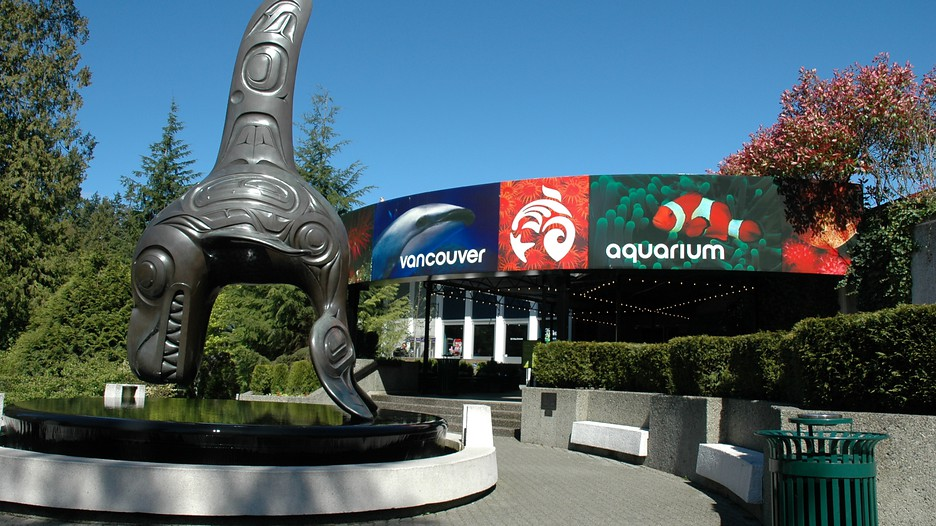
\includegraphics[width=4in]{content/ACL17-vancouver-aquarium.jpg}

\vspace{2ex}\centerline{\rule{.5\linewidth}{.5pt}}\vspace{2ex}
\setlength{\parskip}{1ex}\setlength{\parindent}{0ex}

\daydateyear, 18:00 -- 21:00 \vspace{1em}\\
Vancouver Aquarium (Stanley Park)\\
Vancouver Aquarium\\
845 Avison Way\\
Vancouver, BC\\
V6G 3E2\\
\url{http://www.vanaqua.org/}
\end{center}

\noindent The ACL 2017 Social and Networking Event will be held at the
Vancouver Aquarium located in Stanley Park, on Tuesday, August 1, starting
at 18:00. Here you will enjoy desserts, coffee and tea, and a cash bar.
Bring your kids and enjoy a marine sanctuary in the heart of Stanley Park,
home to thousands of incredible ocean species and amazing aquatic life.
Since opening in 1956, the Vancouver Aquarium has connected more than 40
million people from around the world to our oceans and all the wonders
within them. Enjoy networking with colleagues and have a relaxing evening!


\setdaydateyear{Wednesday}{August 2}{2017}
\chapter{Main Conference: \daydate}
\thispagestyle{emptyheader}
\setheaders{Main Conference}{\daydateyear}

%% Overview page %%%%%%%%%%%%%%%%%%%%%%%%%%%%%%%%%%%%%%%%%%%%%%%%
\section*{Overview}
\renewcommand{\arraystretch}{1.2}
\begin{SingleTrackSchedule}
  9:00 & -- & 10:10 &
  {\bfseries Plenary Session} \hfill \emph{\InvitedLoc}\\
  & & & Invited Talk: Mirella Lapata -- ``Translating from Multiple Modalities to Text and Back''\\
  \\
  10:10 & -- & 10:40 &
  {\bfseries Coffee break} \hfill \emph{\CoffeeLoc}\\
  \\
  10:40 & -- & 12:30 &
  \begin{tabular}{|p{1.65000000000in}|p{1.65000000000in}|}
    \multicolumn{2}{l}{{\bfseries Session 7}}\\\hline
Outstanding Papers 1 & Outstanding Papers 2 \\
\emph{\BestLocA} & \emph{\BestLocB} \\
  \hline\end{tabular} \\
  \\
  12:00 & -- & 13:30 &
  {\bfseries Lunch break} \hfill \emph{\LunchLoc}\\
  \\
  13:00 & -- & 2:30 &
  {\bfseries ACL Business Meeting} \hfill \emph{\BusinessMeetingLoc}\\
  & & & \emph{(Note: overlap)}\\
  \\
  14:30 & -- & 15:00 &
  {\bfseries Coffee break} \hfill \emph{\CoffeeLoc}\\
  \\
  15:00 & -- & 16:45 &
  \begin{tabular}{|p{1.65000000000in}|p{1.65000000000in}|}
    \multicolumn{2}{l}{{\bfseries Session 8}}\\\hline
Outstanding Papers 3 & Outstanding Papers 4 \\
\emph{\BestLocA} & \emph{\BestLocB} \\
  \hline\end{tabular} \\
  \\
  16:45 & -- & 17:45 &
  {\bfseries Lifetime Achievement Award} \hfill \emph{\LifetimeAchievementSessionLoc}\\
  \\
  17:45 & -- & 18:00 &
  {\bfseries Closing Session} \hfill \emph{\ClosingSessionLoc}\\
  \\
\end{SingleTrackSchedule}


%% Sessions  %%%%%%%%%%%%%%%%%%%%%%%%%%%%%%%%%%%%%%%%%%%%%%%%%%%%
\clearpage
\setheaders{Session 7}{\daydateyear}
\begin{TwoSessionOverview}{Session 7}{\daydateyear}
  {Outstanding Papers 1}
  {Outstanding Papers 2}
  \marginnote{\rotatebox{90}{10:40}}[2mm]
  \papertableentry{papers-649} & \papertableentry{papers-733}
  \\
  \hline
  \marginnote{\rotatebox{90}{10:59}}[2mm]
  \papertableentry{papers-193} & \papertableentry{papers-568}
  \\
  \hline
  \marginnote{\rotatebox{90}{11:18}}[2mm]
  \papertableentry{papers-707} & \papertableentry{shortpapers-3580}
  \\
  \hline
  \marginnote{\rotatebox{90}{11:37}}[2mm]
  \papertableentry{shortpapers-3240} & \papertableentry{shortpapers-3410}
  \\
  \hline
  \marginnote{\rotatebox{90}{11:50}}[2mm]
  \papertableentry{shortpapers-3263} & \papertableentry{shortpapers-3417}
  \\
  \hline
  \marginnote{\rotatebox{90}{12:13}}[2mm]
  \papertableentry{shortpapers-3322} & \papertableentry{shortpapers-3452}
  \\
\end{TwoSessionOverview}

\newpage
\section*{Parallel Session 7}
\par\centerline{\bfseries\large Session Session 7A: Outstanding Papers 1}\vspace{1em}\par
\paperabstract{\day}{10:40--10:58}{}{}{papers-649}
\paperabstract{\day}{10:59--11:17}{}{}{papers-193}
\paperabstract{\day}{11:18--11:36}{}{}{papers-707}
\paperabstract{\day}{11:37--11:49}{}{}{shortpapers-3240}
\paperabstract{\day}{11:50--12:12}{}{}{shortpapers-3263}
\paperabstract{\day}{12:13--12:25}{}{}{shortpapers-3322}
\clearpage
\par\centerline{\bfseries\large Session Session 7B: Outstanding Papers 2}\vspace{1em}\par
\paperabstract{\day}{10:40--10:58}{}{}{papers-733}
\paperabstract{\day}{10:59--11:17}{}{}{papers-568}
\paperabstract{\day}{11:18--11:36}{}{}{shortpapers-3580}
\paperabstract{\day}{11:37--11:49}{}{}{shortpapers-3410}
\paperabstract{\day}{11:50--12:12}{}{}{shortpapers-3417}
\paperabstract{\day}{12:13--12:25}{}{}{shortpapers-3452}
\clearpage

\clearpage
\setheaders{Session 8}{\daydateyear}
\begin{TwoSessionOverview}{Session 8}{\daydateyear}
  {Outstanding Papers 3}
  {Outstanding Papers 4}
  \marginnote{\rotatebox{90}{15:00}}[2mm]
  \papertableentry{papers-558} & \papertableentry{papers-222}
  \\
  \hline
  \marginnote{\rotatebox{90}{15:19}}[2mm]
  \papertableentry{papers-732} & \papertableentry{papers-268}
  \\
  \hline
  \marginnote{\rotatebox{90}{15:38}}[2mm]
  \papertableentry{papers-326} & \papertableentry{papers-220}
  \\
  \hline
  \marginnote{\rotatebox{90}{15:57}}[2mm]
  \papertableentry{papers-336} & \papertableentry{papers-638}
  \\
  \hline
  \marginnote{\rotatebox{90}{16:16}}[2mm]
  \papertableentry{papers-578} & \papertableentry{papers-590}
  \\
\end{TwoSessionOverview}

\newpage
\section*{Parallel Session 8}
\par\centerline{\bfseries\large Session Session 8A: Outstanding Papers 3}\vspace{1em}\par
\paperabstract{\day}{15:00--15:18}{}{}{papers-558}
\paperabstract{\day}{15:19--15:37}{}{}{papers-732}
\paperabstract{\day}{15:38--15:56}{}{}{papers-326}
\paperabstract{\day}{15:57--16:15}{}{}{papers-336}
\paperabstract{\day}{16:16--16:34}{}{}{papers-578}
\clearpage
\par\centerline{\bfseries\large Session Session 8B: Outstanding Papers 4}\vspace{1em}\par
\paperabstract{\day}{15:00--15:18}{}{}{papers-222}
\paperabstract{\day}{15:19--15:37}{}{}{papers-268}
\paperabstract{\day}{15:38--15:56}{}{}{papers-220}
\paperabstract{\day}{15:57--16:15}{}{}{papers-638}
\paperabstract{\day}{16:16--16:34}{}{}{papers-590}
\clearpage



%% WORKSHOPS %%%%%%%%%%%%%%%%%%%%%%%%%%%%%%%%%%%%%%%%%%%%%%%%%%%%
\setdaydateyear{Sunday,Thursday--Friday}{July 30,August 3--4}{2017}
\chapter[Workshops and Colocated Events: \daydate]{Workshops and Colocated Events}
\thispagestyle{emptyheader}
\setheaders{Workshops and Colocated Events}{\daydateyear}
\vfill

\begin{center}
\renewcommand{\arraystretch}{1.1}
\vspace{-1em}
\begin{tabular}{@{}%
  >{\raggedright\arraybackslash}p{.3\textwidth}
  >{\raggedright\arraybackslash}p{.65\textwidth}
  >{\raggedleft\arraybackslash}p{.05\textwidth}}

  %% \multicolumn{3}{l}{\hspace{-1mm}\large Monday} \\ \hline
  %% %% \textbf{Room} & \textbf{Name} & \textbf{Page} \\
  %% \SRWLoc & Student Research Workshop & \pageref{SRW} \\
  %% \\

  \multicolumn{3}{l}{\hspace{-1mm}\large Thursday--Friday} \\  \hline
  \WShopLocA & CoNLL: The SIGNLL Conference on Computational Natural Language Learning & p.\pageref{WShopA} \\
  \WShopLocB & *SEM: Sixth Joint Conference On Lexical And Computational Semantics &  p.\pageref{WShopB} \\
  \WShopLocC & SemEval: 11th International Workshop on Semantic Evaluation &  p.\pageref{WShopC} \\
  \\

  \multicolumn{3}{l}{\hspace{-1mm}\large Sunday} \\ \hline
  \WShopLocD & Women and Underrepresented Groups in Natural Language Processing & p.\pageref{WShopD} \\
  \\

  \multicolumn{3}{l}{\hspace{-1mm}\large Thursday} \\ \hline
  \WShopLocE & The 10th Workshop on Building and Using Comparable Corpora & p.\pageref{WShopE} \\
  \WShopLocF & Computational Linguistics and Clinical Psychology – From Linguistic Signal to Clinical Reality & p.\pageref{WShopF} \\
  \WShopLocG & Workshops on Natural Language Processing and Computational Social Science & p.\pageref{WShopG} \\
  \WShopLocH & The 2nd Workshop on Representation Learning for NLP & p.\pageref{WShopH} \\
  \WShopLocI & Language Grounding for Robotics & p.\pageref{WShopI} \\
  \WShopLocJ & Graph-based Methods for Natural Language Processing & p.\pageref{WShopJ} \\
  \\

  \multicolumn{3}{l}{\hspace{-1mm}\large Friday} \\ \hline
  \WShopLocK & The 1st Workshop on Abusive Language Online & p.\pageref{WShopK} \\
  \WShopLocL & Workshop on Biomedical Natural Language Processing & p.\pageref{WShopL} \\
  \WShopLocM & Events and Stories in the News & p.\pageref{WShopM} \\
  \WShopLocN & Joint SIGHUM Workshop on Computational Linguistics for Cultural Heritage, Social Sciences, Humanities and Literature & p.\pageref{WShopN} \\
  \WShopLocO & The 1st Workshop on Neural Machine Translation & p.\pageref{WShopO} \\

\end{tabular}
\end{center}


%% \begin{wsschedule}
%%   {Workshop title}
%%   {Workshop number}
%%   {Workshop label}
%%   {Workshop paper ID}
%%   {Workshop location}
%%   
\item[] {\Large\bfseries Thursday, August 3, 2017}\\\vspace{1.5ex}

\vspace{1ex}
\item[9:00--9:15] {\bfseries  # Welcome and Opening Remarks}

\vspace{1ex}
\item[9:15--9:50] {\bfseries  # Invited Talk 1 (Joyce Chai, MSU)}
\index{Chai, Joyce}

\vspace{1ex}
\item[9:50--10:25] {\bfseries  # Invited Talk 2 (Ray Mooney, UT Austin)}
\index{Mooney, Ray}

\vspace{1ex}
\item[10:30--11:00] {\bfseries  # Coffee break}

\vspace{1ex}
\item[11:00--11:35] {\bfseries  # Invited Talk 3 (Stefanie Tellax)}
\index{Tellax, Stefanie}

\vspace{1ex}
\item[11:35--12:10] {\bfseries  # Invited Talk 4 (Karl Moritz Hermann, Google DeepMind)}
\index{Hermann, Karl Moritz}

\vspace{1ex}
\item[12:10--14:00] {\bfseries  # Poster Session (Lunch from 12:30--14:00)}
\item[$\bullet$] \wspaperentry{RoboNLP-002}
\item[$\bullet$] \wspaperentry{RoboNLP-004}
\item[$\bullet$] \wspaperentry{RoboNLP-005}
\item[$\bullet$] \wspaperentry{RoboNLP-010}
\item[$\bullet$] \wspaperentry{RoboNLP-014}
\item[$\bullet$] \wspaperentry{RoboNLP-017}
\item[$\bullet$] \wspaperentry{RoboNLP-020}
\item[$\bullet$] \wspaperentry{RoboNLP-021}
\item[$\bullet$] \wspaperentry{RoboNLP-023}

\vspace{1ex}
\item[14:00--14:35] {\bfseries  # Invited Talk 5 (Percy Liang, Stanford)}
\index{Liang, Percy}

\vspace{1ex}
\item[14:45--15:10] {\bfseries  # Invited Talk 6 (Jason Weston, Facebook AI Research)}
\index{Weston, Jason}

\vspace{1ex}
\item[] {\bfseries Selected Oral Submission 1}
\item[15:10--15:20] \wspaperentry{RoboNLP-003}

\vspace{1ex}
\item[] {\bfseries Selected Oral Submission 2}
\item[15:20--15:30] \wspaperentry{RoboNLP-006}

\vspace{1ex}
\item[15:30--16:00] {\bfseries  # Coffee break}

\vspace{1ex}
\item[] {\bfseries Selected Oral Submission 3}
\item[16:00--16:10] \wspaperentry{RoboNLP-019}

\vspace{1ex}
\item[16:10--16:45] {\bfseries  # Invited Talk 7 (Nicholas Roy, MIT)}
\index{Roy, Nicholas}

\vspace{1ex}
\item[16:45--17:45] {\bfseries  # Panel}

%% \end{wsschedule}

%%%
% Moved WiNLP to handbook.tex
%%%

%%%
% Colocated
%%%
\setdaydateyear{Thursday--Friday}{August 3--4}{2017}
\setheaders{Two-day Workshops and Colocated Events}{\daydateyear}

\begin{wsschedule}
  {CoNLL: The SIGNLL Conference on Computational Natural Language Learning}
  {1}{WShopA}
  {workshop1}
  {\WShopLocA}
  
\item[] {\Large\bfseries Thursday, August 3, 2017}\\\vspace{1.5ex}

\vspace{1ex}
\item[8:45--9:00] {\bfseries  Opening Remarks}

\vspace{1ex}
\item[] {\bfseries Invited Talk by Chris Dyer}
\item[9:00--10:00] \wspaperentry{CoNLL-291}
\index{Dyer, Chris}

\vspace{1ex}
\item[] {\bfseries Session 1}
\item[10:00--10:15] \wspaperentry{CoNLL-032}

\vspace{1ex}
\item[] {\bfseries Session 1L: Lightning Talks for Poster Session}
\item[10:15--10:17] \wspaperentry{CoNLL-070}
\item[10:17--10:19] \wspaperentry{CoNLL-003}
\item[10:19--10:21] \wspaperentry{CoNLL-181}
\item[10:21--10:23] \wspaperentry{CoNLL-164}
\item[10:23--10:25] \wspaperentry{CoNLL-043}
\item[10:25--10:27] \wspaperentry{CoNLL-047}
\item[10:27--10:29] \wspaperentry{CoNLL-089}
\item[10:29--10:31] \wspaperentry{CoNLL-209}

\vspace{1ex}
\item[10:31--11:00] {\bfseries  Coffee Break}

\vspace{1ex}
\item[] {\bfseries Session ST1: CoNLL-SIGMORPHON Shared Task}

\vspace{1ex}
\item[11:00--12:30] Mans Hulden, Ryan Cotterell, Christo Kirov, and John Sylak-Glassman: Universal Morphological Reinflection in 52 Languages
\index{Hulden, Mans}
\index{Cotterell, Ryan}
\index{Kirov, Christo}
\index{Sylak-Glassman, John}

\vspace{1ex}
\item[12:30--14:00] {\bfseries  Lunch Break}

\vspace{1ex}
\item[] {\bfseries Session ST2: CoNLL Shared Task}

\vspace{1ex}
\item[14:00--15:30] Dan Zeman, Jan Haji\v{c}, et al.: Multilingual Parsing from Raw Text to Universal Dependencies
\index{Zeman, Dan}
\index{Haji\v{c}, Jan}

\vspace{1ex}
\item[15:30--16:00] {\bfseries  Coffee Break}

\vspace{1ex}
\item[] {\bfseries Session 2}
\item[16:00--16:15] \wspaperentry{CoNLL-037}
\item[16:15--16:30] \wspaperentry{CoNLL-066}
\item[16:30--16:45] \wspaperentry{CoNLL-148}
\item[16:45--17:00] \wspaperentry{CoNLL-112}
\item[17:00--17:15] \wspaperentry{CoNLL-152}

\vspace{1ex}
\item[] {\bfseries Session 2L: Lightning Talks for Poster Session}
\item[17:15--17:17] \wspaperentry{CoNLL-198}
\item[17:17--17:19] \wspaperentry{CoNLL-060}
\item[17:19--17:21] \wspaperentry{CoNLL-160}
\item[17:21--17:23] \wspaperentry{CoNLL-284}
\item[17:23--17:25] \wspaperentry{CoNLL-161}
\item[17:25--17:27] \wspaperentry{CoNLL-258}
\item[17:27--17:29] \wspaperentry{CoNLL-212}
\item[17:29--17:31] \wspaperentry{CoNLL-117}

\vspace{1ex}
\item[17:31--18:31] {\bfseries  Business Meeting}

\newpage
\item[] {\Large\bfseries Friday, August 4, 2017}\\\vspace{1.5ex}

\vspace{1ex}
\item[] {\bfseries Invited talk by Naomi Feldman}
\item[8:45--9:45] \wspaperentry{CoNLL-292}
\index{Feldman, Naomi}

\vspace{1ex}
\item[] {\bfseries Session 3}
\item[9:45--10:00] \wspaperentry{CoNLL-179}
\item[10:00--10:15] \wspaperentry{CoNLL-204}

\vspace{1ex}
\item[] {\bfseries Session 3L: Lightning Talks for Poster Session}
\item[10:15--10:17] \wspaperentry{CoNLL-189}
\item[10:17--10:19] \wspaperentry{CoNLL-009}
\item[10:19--10:21] \wspaperentry{CoNLL-013}
\item[10:21--10:23] \wspaperentry{CoNLL-260}
\item[10:23--10:25] \wspaperentry{CoNLL-217}
\item[10:25--10:27] \wspaperentry{CoNLL-052}
\item[10:27--10:29] \wspaperentry{CoNLL-023}

\vspace{1ex}
\item[10:29--11:00] {\bfseries  Coffee Break}

\vspace{1ex}
\item[11:00--14:00] {\bfseries  Poster Session \& Lunch}

\vspace{1ex}
\item[] {\bfseries Session 4}
\item[14:00--14:15] \wspaperentry{CoNLL-038}
\item[14:15--14:30] \wspaperentry{CoNLL-004}
\item[14:30--14:45] \wspaperentry{CoNLL-157}
\item[14:45--15:00] \wspaperentry{CoNLL-045}
\item[15:00--15:15] \wspaperentry{CoNLL-218}
\item[15:15--15:30] \wspaperentry{CoNLL-169}

\vspace{1ex}
\item[15:30--16:00] {\bfseries  Coffee Break}

\vspace{1ex}
\item[] {\bfseries Session 5}
\item[16:00--17:15] \wspaperentry{CoNLL-018}
\item[16:15--16:30] \wspaperentry{CoNLL-110}
\item[16:30--17:45] \wspaperentry{CoNLL-259}
\item[16:45--17:00] \wspaperentry{CoNLL-166}
\item[17:00--17:15] \wspaperentry{CoNLL-042}
\item[17:15--17:30] \wspaperentry{CoNLL-080}

\vspace{1ex}
\item[17:30--17:35] {\bfseries  Best Paper Award}

\vspace{1ex}
\item[17:35--17:45] {\bfseries  Closing Remarks}

\end{wsschedule}

\begin{wsschedule}
  {*SEM: Sixth Joint Conference On Lexical And Computational Semantics}
  {2}{WShopB}
  {workshop2}
  {\WShopLocB}
  
\item[] {\Large\bfseries August 3rd, 2017}\\\vspace{1.5ex}

\vspace{1ex}
\item[9:00--10:30] {\bfseries  Session S1: Invited Talk (Jointly with SemEval) and Best Paper Award}

\vspace{1ex}
\item[9:00--9:15] {\bfseries  Opening Remarks}
\vspace{1ex}
\item[9:15--10:15] {\bfseries  Invited Talk: From Naive Physics to Connotation: Modeling Commonsense in Frame Semantics (Yejin Choi)}

\vspace{1ex}
\item[10:15--10:30] {\bfseries  Announcement of the Adam Kilgarriff Best Paper Award}

\vspace{1ex}
\item[10:30--11:00] {\bfseries  Coffee Break}

\vspace{1ex}
\item[11:00--12:30] {\bfseries  Session S2: Distributional Semantics}
\item[11:00--11:30] \wspaperentry{starSEM-098}
\item[11:30--12:00] \wspaperentry{starSEM-091}
\item[12:00--12:30] \wspaperentry{starSEM-077}

\vspace{1ex}
\item[12:30--2:00] {\bfseries  Lunch Break}

\vspace{1ex}
\item[2:00--3:30] {\bfseries  Session S3: Lexical Semantics and Lexical Resources}
\item[2:00--2:30] \wspaperentry{starSEM-090}
\item[2:30--3:00] \wspaperentry{starSEM-102}
\item[3:00--3:30] \wspaperentry{starSEM-060}

\vspace{1ex}
\item[3:30--4:00] {\bfseries  Coffee Break}

\vspace{1ex}
\item[4:00--4:30] {\bfseries  Session S4: Lexical Semantics and Lexical Resources (continued)}
\item[4:00--4:30] \wspaperentry{starSEM-030}

\vspace{1ex}
\item[4:30--6:00] {\bfseries  Session S5: Poster Session}
\item[$\bullet$] \wspaperentry{starSEM-009}
\item[$\bullet$] \wspaperentry{starSEM-069}
\item[$\bullet$] \wspaperentry{starSEM-005}
\item[$\bullet$] \wspaperentry{starSEM-082}
\item[$\bullet$] \wspaperentry{starSEM-021}
\item[$\bullet$] \wspaperentry{starSEM-081}
\item[$\bullet$] \wspaperentry{starSEM-046}
\item[$\bullet$] \wspaperentry{starSEM-058}
\item[$\bullet$] \wspaperentry{starSEM-034}
\item[$\bullet$] \wspaperentry{starSEM-062}
\item[$\bullet$] \wspaperentry{starSEM-028}
\item[$\bullet$] \wspaperentry{starSEM-003}
\item[$\bullet$] \wspaperentry{starSEM-035}

\vspace{7em}
\item[] {\Large\bfseries August 4th, 2017}\\\vspace{1.5ex}

\vspace{1ex}
\item[9:00--10:30] {\bfseries  Session S6: Invited Talk and Distributional Semantics}
\vspace{1ex}
\item[9:00--10:00] {\bfseries  Invited Talk: What Do You Know About an Alligator When You Know the Company It Keeps? (Katrin Erk)}
\item[10:00--10:30] \wspaperentry{starSEM-055}

\vspace{1ex}
\item[10:30--11:00] {\bfseries  Coffee Break}

\vspace{1ex}
\item[11:00--12:30] {\bfseries  Session S7: Linguistic and Formal Semantics}
\item[11:00--11:30] \wspaperentry{starSEM-064}
\item[11:30--12:00] \wspaperentry{starSEM-027}
\item[12:00--12:30] \wspaperentry{starSEM-018}

\vspace{1ex}
\item[12:30--2:00] {\bfseries  Lunch Break}

\vspace{1ex}
\item[2:00--3:30] {\bfseries  Session S8: Representations of Meaning}
\item[2:00--2:30] \wspaperentry{starSEM-044}
\item[2:30--3:00] \wspaperentry{starSEM-007}
\item[3:00--3:30] \wspaperentry{starSEM-041}

\vspace{1ex}
\item[3:30--4:00] {\bfseries  Coffee Break}

\vspace{1ex}
\item[4:00--5:30] {\bfseries  Session S9: Semantics for Applications}
\item[4:00--4:30] \wspaperentry{starSEM-020}
\item[4:30--5:00] \wspaperentry{starSEM-032}
\item[5:00--5:30] \wspaperentry{starSEM-038}

\vspace{1ex}
\item[5:30--5:40] {\bfseries  Closing Remarks}

\end{wsschedule}

\begin{wsschedule}
  {SemEval: 11th International Workshop on Semantic Evaluation}
  {3}{WShopC}
  {workshop3}
  {\WShopLocC}
  
\item[] {\Large\bfseries 3 August 2017}\\\vspace{1.5ex}

\vspace{1ex}
\item[9:00--9:15] {\bfseries  Welcome / Opening Remarks}
\vspace{1ex}
\item[9:15--10:30] {\bfseries  Invited Talk: From Naive Physics to Connotation: Modeling Commonsense in Frame Semantics (Yejin Choi)}

\vspace{1ex}
\item[10:30--11:00] {\bfseries  Coffee}

\vspace{1ex}
\item[11:00--12:30] {\bfseries  Task Descriptions}
\item[11:00--11:15] \wspaperentry{SemEval-193}
\item[11:15--11:30] \wspaperentry{SemEval-181}
\item[11:30--11:45] \wspaperentry{SemEval-192}
\item[11:45--12:00] \wspaperentry{SemEval-189}
\item[12:00--12:15] \wspaperentry{SemEval-184}
\item[12:15--12:30] \wspaperentry{SemEval-182}

\vspace{1ex}
\item[12:30--2:00] {\bfseries  Lunch}

\vspace{1ex}
\item[2:00--3:30] {\bfseries  Best Of SemEval}
\item[2:00--2:15] \wspaperentry{SemEval-079}
\item[2:15--2:30] \wspaperentry{SemEval-123}
\item[2:30--2:45] \wspaperentry{SemEval-071}
\item[2:45--3:00] \wspaperentry{SemEval-152}
\item[3:00--3:15] \wspaperentry{SemEval-113}
\vspace{1ex}
\item[3:15--3:30] {\bfseries  Turing at SemEval-2017 Task 8: Sequential Approach to Rumour Stance Classification with Branch-LSTM (Elena Kochkina, Maria Liakata and Isabelle Augenstein)}

\vspace{1ex}
\item[3:30--4:00] {\bfseries  Coffee}

\vspace{1ex}
\item[4:00--4:30] {\bfseries  Discussion}

\vspace{1ex}
\item[4:30--5:30] {\bfseries  Poster Session}
\item[4:30--5:30] \wspaperentry{SemEval-007}
\item[4:30--5:30] \wspaperentry{SemEval-008}
\item[4:30--5:30] \wspaperentry{SemEval-050}
\item[4:30--5:30] \wspaperentry{SemEval-058}
\item[4:30--5:30] \wspaperentry{SemEval-059}
\item[4:30--5:30] \wspaperentry{SemEval-063}
\item[4:30--5:30] \wspaperentry{SemEval-065}
\item[4:30--5:30] \wspaperentry{SemEval-072}
\item[4:30--5:30] \wspaperentry{SemEval-073}
\item[4:30--5:30] \wspaperentry{SemEval-080}
\item[4:30--5:30] \wspaperentry{SemEval-081}
\item[4:30--5:30] \wspaperentry{SemEval-089}
\item[4:30--5:30] \wspaperentry{SemEval-107}
\item[4:30--5:30] \wspaperentry{SemEval-127}
\item[4:30--5:30] \wspaperentry{SemEval-135}
\item[4:30--5:30] \wspaperentry{SemEval-143}
\item[4:30--5:30] \wspaperentry{SemEval-151}
\item[4:30--5:30] \wspaperentry{SemEval-158}
\item[4:30--5:30] \wspaperentry{SemEval-172}
\item[4:30--5:30] \wspaperentry{SemEval-174}
\item[4:30--5:30] \wspaperentry{SemEval-054}
\item[4:30--5:30] \wspaperentry{SemEval-010}
\item[4:30--5:30] \wspaperentry{SemEval-017}
\item[4:30--5:30] \wspaperentry{SemEval-046}
\item[4:30--5:30] \wspaperentry{SemEval-077}
\item[4:30--5:30] \wspaperentry{SemEval-102}
\item[4:30--5:30] \wspaperentry{SemEval-114}
\item[4:30--5:30] \wspaperentry{SemEval-125}
\item[4:30--5:30] \wspaperentry{SemEval-157}
\item[4:30--5:30] \wspaperentry{SemEval-161}
\item[4:30--5:30] \wspaperentry{SemEval-167}
\item[4:30--5:30] \wspaperentry{SemEval-002}
\item[4:30--5:30] \wspaperentry{SemEval-009}
\item[4:30--5:30] \wspaperentry{SemEval-016}
\item[4:30--5:30] \wspaperentry{SemEval-021}
\item[4:30--5:30] \wspaperentry{SemEval-032}
\item[4:30--5:30] \wspaperentry{SemEval-038}
\item[4:30--5:30] \wspaperentry{SemEval-051}
\item[4:30--5:30] \wspaperentry{SemEval-052}
\item[4:30--5:30] \wspaperentry{SemEval-057}
\item[4:30--5:30] \wspaperentry{SemEval-083}
\item[4:30--5:30] \wspaperentry{SemEval-094}
\item[4:30--5:30] \wspaperentry{SemEval-106}
\item[4:30--5:30] \wspaperentry{SemEval-126}
\item[4:30--5:30] \wspaperentry{SemEval-145}
\item[4:30--5:30] \wspaperentry{SemEval-146}
\item[4:30--5:30] \wspaperentry{SemEval-159}
\item[4:30--5:30] \wspaperentry{SemEval-162}
\item[4:30--5:30] \wspaperentry{SemEval-163}
\item[4:30--5:30] \wspaperentry{SemEval-170}
\item[4:30--5:30] \wspaperentry{SemEval-178}
\item[4:30--5:30] \wspaperentry{SemEval-004}
\item[4:30--5:30] \wspaperentry{SemEval-031}
\item[4:30--5:30] \wspaperentry{SemEval-118}
\item[4:30--5:30] \wspaperentry{SemEval-122}
\item[4:30--5:30] \wspaperentry{SemEval-149}
\item[4:30--5:30] \wspaperentry{SemEval-160}
\item[4:30--5:30] \wspaperentry{SemEval-179}
\item[4:30--5:30] \wspaperentry{SemEval-001}
\item[4:30--5:30] \wspaperentry{SemEval-022}
\item[4:30--5:30] \wspaperentry{SemEval-024}
\item[4:30--5:30] \wspaperentry{SemEval-033}
\item[4:30--5:30] \wspaperentry{SemEval-055}
\item[4:30--5:30] \wspaperentry{SemEval-074}
\item[4:30--5:30] \wspaperentry{SemEval-075}
\item[4:30--5:30] \wspaperentry{SemEval-111}
\item[4:30--5:30] \wspaperentry{SemEval-168}
\item[4:30--5:30] \wspaperentry{SemEval-169}
\item[4:30--5:30] \wspaperentry{SemEval-023}
\item[4:30--5:30] \wspaperentry{SemEval-053}
\item[4:30--5:30] \wspaperentry{SemEval-132}
\item[4:30--5:30] \wspaperentry{SemEval-139}
\item[4:30--5:30] \wspaperentry{SemEval-141}
\item[4:30--5:30] \wspaperentry{SemEval-148}
\item[4:30--5:30] \wspaperentry{SemEval-164}
\item[4:30--5:30] \wspaperentry{SemEval-171}

\vspace{7em}
\item[] {\Large\bfseries 4 Aug 2017}\\\vspace{1.5ex}

\vspace{1ex}
\item[9:00--9:30] {\bfseries  SemEval 2018 Tasks}

\vspace{1ex}
\item[9:30--10:30] {\bfseries  State of SemEval Discussion}

\vspace{1ex}
\item[10:30--11:00] {\bfseries  Coffee}

\vspace{1ex}
\item[11:00--12:30] {\bfseries  Task Descriptions}
\item[11:00--11:15] \wspaperentry{SemEval-187}
\item[11:15--11:30] \wspaperentry{SemEval-185}
\item[11:30--11:45] \wspaperentry{SemEval-186}
\item[11:45--12:00] \wspaperentry{SemEval-183}
\item[12:00--12:15] \wspaperentry{SemEval-191}
\item[12:15--12:30] \wspaperentry{SemEval-188}

\vspace{1ex}
\item[12:30--2:00] {\bfseries  Lunch}

\vspace{1ex}
\item[2:00--3:30] {\bfseries  Best Of SemEval}
\item[2:00--2:15] \wspaperentry{SemEval-029}
\item[2:15--2:30] \wspaperentry{SemEval-103}
\item[2:30--2:45] \wspaperentry{SemEval-121}
\item[2:45--3:00] \wspaperentry{SemEval-049}
\item[3:00--3:15] \wspaperentry{SemEval-117}

\vspace{1ex}
\item[3:30--4:00] {\bfseries  Coffee}

\vspace{1ex}
\item[4:00--4:30] {\bfseries  Discussion}

\vspace{1ex}
\item[4:30--5:30] {\bfseries  Poster Session}
\item[4:30--5:30] \wspaperentry{SemEval-005}
\item[4:30--5:30] \wspaperentry{SemEval-006}
\item[4:30--5:30] \wspaperentry{SemEval-012}
\item[4:30--5:30] \wspaperentry{SemEval-013}
\item[4:30--5:30] \wspaperentry{SemEval-015}
\item[4:30--5:30] \wspaperentry{SemEval-018}
\item[4:30--5:30] \wspaperentry{SemEval-020}
\item[4:30--5:30] \wspaperentry{SemEval-026}
\item[4:30--5:30] \wspaperentry{SemEval-030}
\item[4:30--5:30] \wspaperentry{SemEval-035}
\item[4:30--5:30] \wspaperentry{SemEval-037}
\item[4:30--5:30] \wspaperentry{SemEval-039}
\item[4:30--5:30] \wspaperentry{SemEval-040}
\item[4:30--5:30] \wspaperentry{SemEval-043}
\item[4:30--5:30] \wspaperentry{SemEval-044}
\item[4:30--5:30] \wspaperentry{SemEval-056}
\item[4:30--5:30] \wspaperentry{SemEval-061}
\item[4:30--5:30] \wspaperentry{SemEval-062}
\item[4:30--5:30] \wspaperentry{SemEval-066}
\item[4:30--5:30] \wspaperentry{SemEval-068}
\item[4:30--5:30] \wspaperentry{SemEval-076}
\item[4:30--5:30] \wspaperentry{SemEval-082}
\item[4:30--5:30] \wspaperentry{SemEval-087}
\item[4:30--5:30] \wspaperentry{SemEval-088}
\item[4:30--5:30] \wspaperentry{SemEval-090}
\item[4:30--5:30] \wspaperentry{SemEval-091}
\item[4:30--5:30] \wspaperentry{SemEval-093}
\item[4:30--5:30] \wspaperentry{SemEval-097}
\item[4:30--5:30] \wspaperentry{SemEval-100}
\item[4:30--5:30] \wspaperentry{SemEval-105}
\item[4:30--5:30] \wspaperentry{SemEval-108}
\item[4:30--5:30] \wspaperentry{SemEval-110}
\item[4:30--5:30] \wspaperentry{SemEval-119}
\item[4:30--5:30] \wspaperentry{SemEval-120}
\item[4:30--5:30] \wspaperentry{SemEval-134}
\item[4:30--5:30] \wspaperentry{SemEval-142}
\item[4:30--5:30] \wspaperentry{SemEval-147}
\item[4:30--5:30] \wspaperentry{SemEval-154}
\item[4:30--5:30] \wspaperentry{SemEval-166}
\item[4:30--5:30] \wspaperentry{SemEval-019}
\item[4:30--5:30] \wspaperentry{SemEval-025}
\item[4:30--5:30] \wspaperentry{SemEval-028}
\item[4:30--5:30] \wspaperentry{SemEval-064}
\item[4:30--5:30] \wspaperentry{SemEval-069}
\item[4:30--5:30] \wspaperentry{SemEval-096}
\item[4:30--5:30] \wspaperentry{SemEval-098}
\item[4:30--5:30] \wspaperentry{SemEval-115}
\item[4:30--5:30] \wspaperentry{SemEval-116}
\item[4:30--5:30] \wspaperentry{SemEval-129}
\item[4:30--5:30] \wspaperentry{SemEval-130}
\item[4:30--5:30] \wspaperentry{SemEval-138}
\item[4:30--5:30] \wspaperentry{SemEval-144}
\item[4:30--5:30] \wspaperentry{SemEval-155}
\item[4:30--5:30] \wspaperentry{SemEval-165}
\item[4:30--5:30] \wspaperentry{SemEval-175}
\item[4:30--5:30] \wspaperentry{SemEval-176}
\item[4:30--5:30] \wspaperentry{SemEval-177}
\item[4:30--5:30] \wspaperentry{SemEval-034}
\item[4:30--5:30] \wspaperentry{SemEval-045}
\item[4:30--5:30] \wspaperentry{SemEval-086}
\item[4:30--5:30] \wspaperentry{SemEval-092}
\item[4:30--5:30] \wspaperentry{SemEval-101}
\item[4:30--5:30] \wspaperentry{SemEval-014}
\item[4:30--5:30] \wspaperentry{SemEval-060}
\item[4:30--5:30] \wspaperentry{SemEval-078}
\item[4:30--5:30] \wspaperentry{SemEval-084}
\item[4:30--5:30] \wspaperentry{SemEval-085}
\item[4:30--5:30] \wspaperentry{SemEval-099}
\item[4:30--5:30] \wspaperentry{SemEval-109}
\item[4:30--5:30] \wspaperentry{SemEval-124}
\item[4:30--5:30] \wspaperentry{SemEval-133}
\item[4:30--5:30] \wspaperentry{SemEval-137}
\item[4:30--5:30] \wspaperentry{SemEval-150}
\item[4:30--5:30] \wspaperentry{SemEval-153}
\item[4:30--5:30] \wspaperentry{SemEval-173}
\item[4:30--5:30] \wspaperentry{SemEval-190}
\item[4:30--5:30] \wspaperentry{SemEval-180}
\item[4:30--5:30] \wspaperentry{SemEval-011}
\item[4:30--5:30] \wspaperentry{SemEval-027}
\item[4:30--5:30] \wspaperentry{SemEval-036}
\item[4:30--5:30] \wspaperentry{SemEval-095}
\item[4:30--5:30] \wspaperentry{SemEval-128}
\item[4:30--5:30] \wspaperentry{SemEval-156}

\end{wsschedule}

%%%
% Thursday
%%%
\setdaydateyear{Thursday}{August 3}{2017}
\setheaders{One-day Workshops}{\daydateyear}

\begin{wsschedule}
  {BUCC: 10th Workshop on Building and Using Comparable Corpora}
  {5}{WShopE}
  {workshop5}
  {\WShopLocE}
  \item[$\bullet$] \wspaperentry{BUCC-018}
\item[$\bullet$] \wspaperentry{BUCC-007}
\item[$\bullet$] \wspaperentry{BUCC-013}
\item[$\bullet$] \wspaperentry{BUCC-012}
\item[$\bullet$] \wspaperentry{BUCC-008}
\item[$\bullet$] \wspaperentry{BUCC-010}
\item[$\bullet$] \wspaperentry{BUCC-011}
\item[$\bullet$] \wspaperentry{BUCC-014}
\item[$\bullet$] \wspaperentry{BUCC-015}
\item[$\bullet$] \wspaperentry{BUCC-016}
\item[$\bullet$] \wspaperentry{BUCC-017}
\item[$\bullet$] \wspaperentry{BUCC-019}

\end{wsschedule}

\begin{wsschedule}
  {CLPsych: Computational Linguistics and Clinical Psychology – From Linguistic Signal to Clinical Reality}
  {6}{WShopF}
  {workshop6}
  {\WShopLocF}
  
\item[] {\Large\bfseries Thursday August 3, 2017}\\\vspace{1.5ex}

\vspace{1ex}
\item[9:00--9:20] {\bfseries  Opening Remarks (Kristy Hollingshead, Molly E. Ireland, and Kate Loveys)}

\vspace{1ex}
\item[9:20--10:30] {\bfseries  Session: Oral Presentations 1}
\item[$\bullet$] \wspaperentry{CLPsych-106}
\item[$\bullet$] \wspaperentry{CLPsych-119}

\vspace{1ex}
\item[11:00--12:15] {\bfseries  Session: Poster Presentations}
\item[$\bullet$] \wspaperentry{CLPsych-111}
\item[$\bullet$] \wspaperentry{CLPsych-110}

\vspace{1ex}
\item[1:45--2:30] {\bfseries  Session: Mini-Oral Presentations}
\item[$\bullet$] \wspaperentry{CLPsych-101}
\item[$\bullet$] \wspaperentry{CLPsych-107}
\item[$\bullet$] \wspaperentry{CLPsych-104}
\item[$\bullet$] \wspaperentry{CLPsych-121}

\vspace{1ex}
\item[2:30--3:30] {\bfseries  Session: Oral Presentations 2}
\item[$\bullet$] \wspaperentry{CLPsych-125}
\item[$\bullet$] \wspaperentry{CLPsych-115}

\vspace{1ex}
\item[4:00--5:00] {\bfseries  CLPsych2017 Shared Task: Results \& Open Discussion (David Milne)}

\vspace{1ex}
\item[5:00--5:30] {\bfseries  Closing Remarks}

\end{wsschedule}

\begin{wsschedule}
  {NLP+CSS: Workshops on Natural Language Processing and Computational Social Science}
  {7}{WShopG}
  {workshop7}
  {\WShopLocG}
  
\vspace{1ex}
\item[9:00--10:30] {\bfseries  Session 1}
\vspace{1ex}
\item[9:00--9:15] {\bfseries  Welcome (Organizers)}

\vspace{1ex}
\item[9:15--10:00] {\bfseries  Invited Talk 1}

\vspace{1ex}
\item[10:00--10:30] {\bfseries  Spotlight Paper Session}
\item[10:00--10:15] \wspaperentry{NLPandCSS-014}
\item[10:15--10:30] \wspaperentry{NLPandCSS-013}

\vspace{1ex}
\item[10:30--11:00] {\bfseries  Morning coffee break}

\vspace{1ex}
\item[11:00--12:15] {\bfseries  Session 2}
\vspace{1ex}
\item[11:00--11:45] {\bfseries  Invited Talk: Measuring Psychological Traits using Social Media (Lyle Ungar)}

\vspace{1ex}
\item[11:45--12:15] {\bfseries  Spotlight Paper Session}
\item[11:45--12:00] \wspaperentry{NLPandCSS-030}
\vspace{1ex}
\item[12:00--12:15] {\bfseries  Never Tell Me the Odds: How Belief Dynamics Shape Audience Experience (non-archival) (Shengli Hu)}

\vspace{1ex}
\item[12:15--2:00] {\bfseries  Lunch break}

\vspace{1ex}
\item[2:00--3:30] {\bfseries  Session 3}
\vspace{1ex}
\item[2:00--2:45] {\bfseries  Invited Talk: The War on Facts (Gideon Mann)}

\vspace{1ex}
\item[2:45--3:30] {\bfseries  One-minute-madness paper presentation}
\item[2:45--2:48] \wspaperentry{NLPandCSS-006}
\item[2:48--2:51] \wspaperentry{NLPandCSS-008}
\item[2:51--2:54] \wspaperentry{NLPandCSS-017}
\vspace{1ex}
\item[2:54--2:57] {\bfseries  The Role of Network Structure for Gender Prediction (non-archival) (Kristen M. Altenburger and Johan Ugander)}
\vspace{1ex}
\item[2:57--3:00] {\bfseries  The Role of Party and Incumbency in Identification of Argumentation Strategies in Political Debate (non-archival) (Justin Garten, Kenji Sagae, Zahra Kamel, Nitika Awasthi and Morteza Dehghani)}
\item[3:00--3:03] \wspaperentry{NLPandCSS-021}
\item[3:03--3:06] \wspaperentry{NLPandCSS-028}
\item[3:06--3:09] \wspaperentry{NLPandCSS-029}
\vspace{1ex}
\item[3:09--3:12] {\bfseries  Syntactic Alignment in Power Relations (non-archival) (Reihane Boghrati, Justin Garten and Morteza Dehghani)}
\item[3:12--3:15] \wspaperentry{NLPandCSS-032}
\item[3:15--3:18] \wspaperentry{NLPandCSS-033}
\item[3:18--3:21] \wspaperentry{NLPandCSS-037}
\item[3:21--3:24] \wspaperentry{NLPandCSS-038}
\vspace{1ex}
\item[3:24--3:27] {\bfseries  Market Evolution of Sharing Economy vs. Traditional Platforms: A Natural Language Processing Approach (Mohsen Mosleh and Babak Heydari)}

\vspace{1ex}
\item[3:30--4:45] {\bfseries  Coffee break and posters}

\vspace{1ex}
\item[4:45--5:45] {\bfseries  Session 4}
\vspace{1ex}
\item[4:45--5:30] {\bfseries  Invited Talk (Brandon Stewart)}
\vspace{1ex}
\item[5:30--5:45] {\bfseries  Closing remarks and wrap-up (Organizers)}

\end{wsschedule}

\begin{wsschedule}
  {Repl4NLP: 2nd Workshop on Representation Learning for NLP}
  {8}{WShopH}
  {workshop8}
  {\WShopLocH}
  
\item[] {\Large\bfseries Thursday, August 3, 2017}\\\vspace{1.5ex}

\vspace{1ex}
\item[9:30--9:45] {\bfseries  Welcome and Opening Remarks}

\vspace{1ex}
\item[9:45--10:30] {\bfseries  Keynote Session}
\vspace{1ex}
\item[9:45--10:30] Learning Joint Embeddings of Vision and Language (Sanja Fidler)
\index{Fidler, Sanja}

\vspace{1ex}
\item[10:30--11:00] {\bfseries  Coffee Break}

\vspace{1ex}
\item[11:00--12:30] {\bfseries  Keynote Session}
\vspace{1ex}
\item[11:00--11:45] Learning Representations of Social Meaning (Jacob Eisenstein)
\index{Eisenstein, Jacob}
\vspace{1ex}
\item[11:45--12:30] Representations in the Brain (Alona Fyshe)
\index{Fyshe, Alona}

\vspace{1ex}
\item[12:30--14:00] {\bfseries  Lunch}

\vspace{1ex}
\item[14:00--14:45] {\bfseries  Keynote Session}
\vspace{1ex}
\item[14:00--14:45] ``A million ways to say I love you'' or Learning to Paraphrase with Neural Machine Translation (Mirella Lapata)
\index{Lapata, Mirella}

\vspace{1ex}
\item[14:45--15:00] {\bfseries  Best Paper Session}

\vspace{1ex}
\item[15:00--16:30] {\bfseries  Poster Session, including Coffee Break}
\item[$\bullet$] \wspaperentry{Repl4NLP-006}
\item[$\bullet$] \wspaperentry{Repl4NLP-008}
\item[$\bullet$] \wspaperentry{Repl4NLP-011}
\item[$\bullet$] \wspaperentry{Repl4NLP-013}
\item[$\bullet$] \wspaperentry{Repl4NLP-017}
\item[$\bullet$] \wspaperentry{Repl4NLP-018}
\item[$\bullet$] \wspaperentry{Repl4NLP-019}
\item[$\bullet$] \wspaperentry{Repl4NLP-022}
\item[$\bullet$] \wspaperentry{Repl4NLP-023}
\item[$\bullet$] \wspaperentry{Repl4NLP-026}
\item[$\bullet$] \wspaperentry{Repl4NLP-027}
\item[$\bullet$] \wspaperentry{Repl4NLP-030}
\item[$\bullet$] \wspaperentry{Repl4NLP-032}
\item[$\bullet$] \wspaperentry{Repl4NLP-033}
\item[$\bullet$] \wspaperentry{Repl4NLP-034}
\item[$\bullet$] \wspaperentry{Repl4NLP-035}
\item[$\bullet$] \wspaperentry{Repl4NLP-036}
\item[$\bullet$] \wspaperentry{Repl4NLP-037}
\item[$\bullet$] \wspaperentry{Repl4NLP-041}
\item[$\bullet$] \wspaperentry{Repl4NLP-042}
\item[$\bullet$] \wspaperentry{Repl4NLP-043}
\item[$\bullet$] \wspaperentry{Repl4NLP-045}
\item[$\bullet$] \wspaperentry{Repl4NLP-046}
\item[$\bullet$] \wspaperentry{Repl4NLP-047}
\item[$\bullet$] \wspaperentry{Repl4NLP-048}
\item[$\bullet$] \wspaperentry{Repl4NLP-049}
\item[$\bullet$] \wspaperentry{Repl4NLP-050}
\item[$\bullet$] \wspaperentry{Repl4NLP-053}
\item[$\bullet$] \wspaperentry{Repl4NLP-054}
\item[$\bullet$] \wspaperentry{Repl4NLP-055}
\item[$\bullet$] \wspaperentry{Repl4NLP-056}
\item[$\bullet$] \wspaperentry{Repl4NLP-057}
\item[$\bullet$] \wspaperentry{Repl4NLP-059}
\item[$\bullet$] \wspaperentry{Repl4NLP-060}
\item[$\bullet$] \wspaperentry{Repl4NLP-061}
\item[$\bullet$] \wspaperentry{Repl4NLP-062}
\item[$\bullet$] \wspaperentry{Repl4NLP-064}
\item[$\bullet$] \wspaperentry{Repl4NLP-065}
\item[$\bullet$] \wspaperentry{Repl4NLP-067}
\item[$\bullet$] \wspaperentry{Repl4NLP-066}

\vspace{1ex}
\item[16:30--17:30] {\bfseries  Panel Discussion}

\vspace{1ex}
\item[17:30--17:40] {\bfseries  Closing Remarks}

\end{wsschedule}

\begin{wsschedule}
  {RoboNLP: Language Grounding for Robotics}
  {9}{WShopI}
  {workshop9}
  {\WShopLocI}
  
\item[] {\Large\bfseries Thursday, August 3, 2017}\\\vspace{1.5ex}

\vspace{1ex}
\item[9:00--9:15] {\bfseries  # Welcome and Opening Remarks}

\vspace{1ex}
\item[9:15--9:50] {\bfseries  # Invited Talk 1 (Joyce Chai, MSU)}
\index{Chai, Joyce}

\vspace{1ex}
\item[9:50--10:25] {\bfseries  # Invited Talk 2 (Ray Mooney, UT Austin)}
\index{Mooney, Ray}

\vspace{1ex}
\item[10:30--11:00] {\bfseries  # Coffee break}

\vspace{1ex}
\item[11:00--11:35] {\bfseries  # Invited Talk 3 (Stefanie Tellax)}
\index{Tellax, Stefanie}

\vspace{1ex}
\item[11:35--12:10] {\bfseries  # Invited Talk 4 (Karl Moritz Hermann, Google DeepMind)}
\index{Hermann, Karl Moritz}

\vspace{1ex}
\item[12:10--14:00] {\bfseries  # Poster Session (Lunch from 12:30--14:00)}
\item[$\bullet$] \wspaperentry{RoboNLP-002}
\item[$\bullet$] \wspaperentry{RoboNLP-004}
\item[$\bullet$] \wspaperentry{RoboNLP-005}
\item[$\bullet$] \wspaperentry{RoboNLP-010}
\item[$\bullet$] \wspaperentry{RoboNLP-014}
\item[$\bullet$] \wspaperentry{RoboNLP-017}
\item[$\bullet$] \wspaperentry{RoboNLP-020}
\item[$\bullet$] \wspaperentry{RoboNLP-021}
\item[$\bullet$] \wspaperentry{RoboNLP-023}

\vspace{1ex}
\item[14:00--14:35] {\bfseries  # Invited Talk 5 (Percy Liang, Stanford)}
\index{Liang, Percy}

\vspace{1ex}
\item[14:45--15:10] {\bfseries  # Invited Talk 6 (Jason Weston, Facebook AI Research)}
\index{Weston, Jason}

\vspace{1ex}
\item[] {\bfseries Selected Oral Submission 1}
\item[15:10--15:20] \wspaperentry{RoboNLP-003}

\vspace{1ex}
\item[] {\bfseries Selected Oral Submission 2}
\item[15:20--15:30] \wspaperentry{RoboNLP-006}

\vspace{1ex}
\item[15:30--16:00] {\bfseries  # Coffee break}

\vspace{1ex}
\item[] {\bfseries Selected Oral Submission 3}
\item[16:00--16:10] \wspaperentry{RoboNLP-019}

\vspace{1ex}
\item[16:10--16:45] {\bfseries  # Invited Talk 7 (Nicholas Roy, MIT)}
\index{Roy, Nicholas}

\vspace{1ex}
\item[16:45--17:45] {\bfseries  # Panel}

\end{wsschedule}

\begin{wsschedule}
  {TextGraphs-11: Graph-based Methods for Natural Language Processing}
  {10}{WShopJ}
  {workshop10}
  {\WShopLocJ}
  
\item[] {\Large\bfseries Thursday, August 3, 2017}\\\vspace{1.5ex}
\vspace{1ex}
\item[9:00--9:10] {\bfseries  Opening remarks (Swapna Somasundaran and Goran Glavaš)}
\vspace{1ex}
\item[9:10--10:10] {\bfseries  Invited talk (Apoorv Agarwal)}
\item[10:10--10:30] \wspaperentry{TextGraphs-11-014}

\vspace{1ex}
\item[10:30--11:00] {\bfseries  Coffee break}
\item[11:00--11:20] \wspaperentry{TextGraphs-11-002}
\item[11:20--11:40] \wspaperentry{TextGraphs-11-011}
\item[11:40--12:00] \wspaperentry{TextGraphs-11-008}
\item[12:00--12:15] \wspaperentry{TextGraphs-11-007}

\vspace{1ex}
\item[12:15--14:00] {\bfseries  Lunch}
\vspace{1ex}
\item[14:00--15:00] {\bfseries  Invited talk (Michael Strube)}
\item[15:00--15:15] \wspaperentry{TextGraphs-11-020}
\item[15:15--15:30] \wspaperentry{TextGraphs-11-009}

\vspace{1ex}
\item[15:30--16:00] {\bfseries  Coffee break}
\item[16:00--16:20] \wspaperentry{TextGraphs-11-013}
\item[16:20--16:40] \wspaperentry{TextGraphs-11-022}
\item[16:40--17:00] \wspaperentry{TextGraphs-11-004}
\vspace{1ex}
\item[17:00--17:10] {\bfseries  Best paper award and closing remarks (Swapna Somasundaran and Goran Glavaš)}

\end{wsschedule}

%%%
% Friday
%%%
\setdaydateyear{Friday}{August 4}{2017}
\setheaders{One-day Workshops}{\daydateyear}

\begin{wsschedule}
  {ALW1: 1st Workshop on Abusive Language Online}
  {11}{WShopK}
  {workshop11}
  {\WShopLocK}
  
\item[] {\Large\bfseries Friday, August 4, 2017}\\\vspace{1.5ex}

\vspace{1ex}
\item[8:45--9:05] {\bfseries  Opening Remarks}

\vspace{1ex}
\item[9:05--9:50] {\bfseries  Invited Talk A: Carol Todd}
\index{Todd, Carol}

\vspace{1ex}
\item[9:50--10:35] {\bfseries  Panel A: Sora Han, Liz Losh, Lucas Dixon}
\index{Han, Sora}
\index{Losh, Liz}
\index{Dixon, Lucas}

\vspace{1ex}
\item[10:35--11:00] {\bfseries  Break}

\vspace{1ex}
\item[11:00--12:30] {\bfseries  Paper Presentations}
\item[11:00--11:20] \wspaperentry{ALW1-011}
\item[11:20--11:40] \wspaperentry{ALW1-014}
\item[11:40--12:00] \wspaperentry{ALW1-018}
\item[12:00--12:20] \wspaperentry{ALW1-005}

\vspace{1ex}
\item[12:20--14:00] {\bfseries  Lunch}

\vspace{1ex}
\item[14:00--15:30] {\bfseries  Poster Session}
\item[$\bullet$] \wspaperentry{ALW1-004}
\item[$\bullet$] \wspaperentry{ALW1-007}
\item[$\bullet$] \wspaperentry{ALW1-009}
\item[$\bullet$] \wspaperentry{ALW1-010}
\item[$\bullet$] \wspaperentry{ALW1-016}
\item[$\bullet$] \wspaperentry{ALW1-017}
\item[$\bullet$] \wspaperentry{ALW1-019}
\item[$\bullet$] \wspaperentry{ALW1-021}
\item[$\bullet$] \wspaperentry{ALW1-023}
\item[$\bullet$] \wspaperentry{ALW1-024}

\vspace{1ex}
\item[15:30--16:00] {\bfseries  Break}

\vspace{1ex}
\item[16:00--16:45] {\bfseries  Invited Talk B: Brianna Wu}
\index{Wu, Brianna}

\vspace{1ex}
\item[16:45--17:30] {\bfseries  Panel B: Pascale Fung, Vinodkumar Prabhakaran, Jacqueline Wernimont, Margeret Mitchell}
\index{Fung, Pascale}
\index{Prabhakaran, Vinodkumar}
\index{Wernimont, Jacqueline}
\index{Mitchell, Margeret}

\vspace{1ex}
\item[17:30--17:40] {\bfseries  Closing Remarks}

\end{wsschedule}

\begin{wsschedule}
  {BioNLP: Workshop on Biomedical Natural Language Processing}
  {12}{WShopL}
  {workshop12}
  {\WShopLocL}
  
\item[] {\Large\bfseries Friday August 4, 2017}\\\vspace{1.5ex}

\vspace{1ex}
\item[8:30--8:45] {\bfseries  Opening remarks}

\vspace{1ex}
\item[8:45--10:30] {\bfseries  Session 1: Prediction and relation extraction}
\item[8:45--9:00] \wspaperentry{BioNLP-066}
\item[9:00--9:15] \wspaperentry{BioNLP-045}
\item[9:15--9:30] \wspaperentry{BioNLP-019}
\item[9:30--9:45] \wspaperentry{BioNLP-006}
\item[9:45--10:00] \wspaperentry{BioNLP-004}

\vspace{1ex}
\item[10:00--10:30] {\bfseries  Invited Talk: ``Results of the 5th edition of BioASQ Challenge''  -- Georgios Paliouras}
\item[$\bullet$] \wspaperentry{BioNLP-068}

\vspace{1ex}
\item[10:30--11:00] {\bfseries  Coffee Break}

\vspace{1ex}
\item[11:00--12:30] {\bfseries  Session 2:  BioASQ 2017 and more}
\item[11:00--11:15] \wspaperentry{BioNLP-023}
\item[11:15--11:30] \wspaperentry{BioNLP-044}
\item[11:30--11:45] \wspaperentry{BioNLP-002}
\item[11:45--12:00] \wspaperentry{BioNLP-046}
\item[12:00--12:15] \wspaperentry{BioNLP-003}
\item[12:15--12:30] \wspaperentry{BioNLP-056}

\vspace{1ex}
\item[12:30--2:00] {\bfseries  Lunch break}

\vspace{1ex}
\item[2:00--3:30] {\bfseries  Session 3: From bio to clinical NLP}
\item[2:00--2:15] \wspaperentry{BioNLP-052}
\item[2:15--2:30] \wspaperentry{BioNLP-041}
\item[2:30--2:45] \wspaperentry{BioNLP-030}
\item[2:45--3:00] \wspaperentry{BioNLP-053}
\item[3:00--3:15] \wspaperentry{BioNLP-013}
\item[3:15--3:30] \wspaperentry{BioNLP-032}

\vspace{1ex}
\item[3:30--4:00] {\bfseries  Coffee Break}

\vspace{1ex}
\item[4:00--4:30] {\bfseries  Session 4 More clinical NLP}
\item[4:00--4:15] \wspaperentry{BioNLP-034}
\item[4:15--4:30] \wspaperentry{BioNLP-015}

\vspace{1ex}
\item[4:30--6:00] {\bfseries  Poster Session}
\item[$\bullet$] \wspaperentry{BioNLP-067}
\item[$\bullet$] \wspaperentry{BioNLP-057}
\item[$\bullet$] \wspaperentry{BioNLP-060}
\item[$\bullet$] \wspaperentry{BioNLP-027}
\item[$\bullet$] \wspaperentry{BioNLP-001}
\item[$\bullet$] \wspaperentry{BioNLP-051}
\item[$\bullet$] \wspaperentry{BioNLP-012}
\item[$\bullet$] \wspaperentry{BioNLP-021}
\item[$\bullet$] \wspaperentry{BioNLP-024}
\item[$\bullet$] \wspaperentry{BioNLP-033}
\item[$\bullet$] \wspaperentry{BioNLP-043}
\item[$\bullet$] \wspaperentry{BioNLP-009}
\item[$\bullet$] \wspaperentry{BioNLP-031}
\item[$\bullet$] \wspaperentry{BioNLP-050}
\item[$\bullet$] \wspaperentry{BioNLP-037}
\item[$\bullet$] \wspaperentry{BioNLP-028}
\item[$\bullet$] \wspaperentry{BioNLP-005}
\item[$\bullet$] \wspaperentry{BioNLP-014}
\item[$\bullet$] \wspaperentry{BioNLP-029}
\item[$\bullet$] \wspaperentry{BioNLP-017}
\item[$\bullet$] \wspaperentry{BioNLP-008}
\item[$\bullet$] \wspaperentry{BioNLP-039}
\item[$\bullet$] \wspaperentry{BioNLP-049}
\item[$\bullet$] \wspaperentry{BioNLP-042}
\item[$\bullet$] \wspaperentry{BioNLP-059}
\item[$\bullet$] \wspaperentry{BioNLP-022}
\item[$\bullet$] \wspaperentry{BioNLP-055}
\item[$\bullet$] \wspaperentry{BioNLP-047}

\end{wsschedule}

\begin{wsschedule}
  {EventStory: Events and Stories in the News}
  {13}{WShopM}
  {workshop13}
  {\WShopLocM}
  
\item[] {\Large\bfseries Friday, August 4, 2017}\\\vspace{1.5ex}

\vspace{1ex}
\item[9:00--10:30] {\bfseries  Session 1: }

\vspace{1ex}
\item[9:00--9:05] {\bfseries  Welcome and Opening Remarks}
\vspace{1ex}
\item[9:05--10:05] {\bfseries  A theory of events unifying semantic parsing and reasoning (James F. Allen, University of Rocherster)}
\item[10:05--10:30] \wspaperentry{EventStory-002}

\vspace{1ex}
\item[10:30--11:00] {\bfseries  Coffee Break}

\vspace{1ex}
\item[11:00--12:30] {\bfseries  Session 2: }

\vspace{1ex}
\item[11:00--12:30] {\bfseries  Annotation Exercise}

\vspace{1ex}
\item[12:30--2:00] {\bfseries  Lunch}

\vspace{1ex}
\item[2:00--4:00] {\bfseries  Session 3: }
\item[2:00--2:05] \wspaperentry{EventStory-004}
\item[2:05--2:10] \wspaperentry{EventStory-017}
\item[2:10--2:15] \wspaperentry{EventStory-016}
\item[2:15--2:20] \wspaperentry{EventStory-010}
\item[2:20--2:25] \wspaperentry{EventStory-024}
\item[2:25--2:30] \wspaperentry{EventStory-014}
\item[2:30--2:35] \wspaperentry{EventStory-019}
\item[2:35--2:40] \wspaperentry{EventStory-015}
\item[2:40--2:45] \wspaperentry{EventStory-008}

\vspace{1ex}
\item[2:45--4:00] {\bfseries  Poster session}

\vspace{1ex}
\item[3:30--4:00] {\bfseries  Coffee Break}

\vspace{1ex}
\item[4:00--5:45] {\bfseries  Session 4: }
\item[4:00--4:25] \wspaperentry{EventStory-023}
\item[4:25--4:50] \wspaperentry{EventStory-011}
\item[4:50--5:15] \wspaperentry{EventStory-013}

\vspace{1ex}
\item[5:15--5:45] {\bfseries  Discussion and Conclusion}

\end{wsschedule}

\begin{wsschedule}
  {LaTeCH-CLfL: Joint SIGHUM Workshop on Computational Linguistics for Cultural Heritage, Social Sciences, Humanities and Literature}
  {14}{WShopN}
  {workshop14}
  {\WShopLocN}
  
\item[] {\Large\bfseries August 4th, 2017}\\\vspace{1.5ex}

\vspace{1ex}
\item[9:00--10:00] {\bfseries  Session 1}
\item[9:00--9:30] \wspaperentry{LaTeCH-CLfL-003}
\item[9:30--10:00] \wspaperentry{LaTeCH-CLfL-011}

\vspace{1ex}
\item[10:00--10:30] {\bfseries  Poster Teaser Talks}

\vspace{1ex}
\item[11:00--12:30] {\bfseries  Session 2}
\item[11:00--11:30] \wspaperentry{LaTeCH-CLfL-015}
\item[11:30--12:00] \wspaperentry{LaTeCH-CLfL-022}
\item[12:00--12:30] \wspaperentry{LaTeCH-CLfL-001}

\vspace{1ex}
\item[1:30--2:00] {\bfseries  SIGHUM Business Meeting}

\vspace{1ex}
\item[2:00--3:00] {\bfseries  Invited Talk}
\vspace{1ex}
\item[2:00--3:00] {\bfseries  Characterization (Andrew Piper)}

\vspace{1ex}
\item[3:00--4:00] {\bfseries  Poster Session}
\item[3:00--4:00] \wspaperentry{LaTeCH-CLfL-004}
\item[3:00--4:00] \wspaperentry{LaTeCH-CLfL-008}
\item[3:00--4:00] \wspaperentry{LaTeCH-CLfL-013}
\item[3:00--4:00] \wspaperentry{LaTeCH-CLfL-017}
\item[3:00--4:00] \wspaperentry{LaTeCH-CLfL-019}
\item[3:00--4:00] \wspaperentry{LaTeCH-CLfL-025}
\item[3:00--4:00] \wspaperentry{LaTeCH-CLfL-026}

\vspace{1ex}
\item[4:00--5:30] {\bfseries  Session 4}
\item[4:00--4:30] \wspaperentry{LaTeCH-CLfL-007}
\item[4:30--5:00] \wspaperentry{LaTeCH-CLfL-010}
\item[5:00--5:30] \wspaperentry{LaTeCH-CLfL-027}

\end{wsschedule}

\begin{wsschedule}
  {NMT: 1st Workshop on Neural Machine Translation}
  {15}{WShopO}
  {workshop15}
  {\WShopLocO}
  
\item[] {\Large\bfseries Friday, August 4, 2017}\\\vspace{1.5ex}

\vspace{1ex}
\item[] {\bfseries Session 1}

\vspace{1ex}
\item[9:30--9:40] {\bfseries  Welcome and Opening Remarks}

\vspace{1ex}
\item[9:40--10:30] {\bfseries  Keynote (Chris Dyer)}
\index{Dyer, Chris}
\vspace{1ex}
\item[10:30--11:00] {\bfseries  Coffee Break}

\vspace{1ex}
\item[] {\bfseries Session 2}

\vspace{1ex}
\item[11:00--11:50] {\bfseries  Keynote (Alexander Rush)}
\index{Rush, Alexander}

\vspace{1ex}
\item[11:50--12:20] {\bfseries  Best Paper Session}
\vspace{1ex}
\item[12:20--13:40] {\bfseries  Lunch Break}

\vspace{1ex}
\item[] {\bfseries Session 3}

\vspace{1ex}
\item[13:40--14:30] {\bfseries  Keynote (Kevin Knight)}
\index{Knight, Kevin}

\vspace{1ex}
\item[14:30-15:20] {\bfseries  Keynote (Quoc Le)}
\index{Le, Quoc}

\vspace{1ex}
\item[] {\bfseries Session 4}

\vspace{1ex}
\item[15:20--15:30] {\bfseries  Poster Session}
\item[$\bullet$] \wspaperentry{NMT-004}
\item[$\bullet$] \wspaperentry{NMT-003}
\item[$\bullet$] \wspaperentry{NMT-010}
\item[$\bullet$] \wspaperentry{NMT-021}
\item[$\bullet$] \wspaperentry{NMT-012}
\item[$\bullet$] \wspaperentry{NMT-013}
\item[$\bullet$] \wspaperentry{NMT-017}
\item[$\bullet$] \wspaperentry{NMT-007}
\item[$\bullet$] \wspaperentry{NMT-008}
\item[$\bullet$] \wspaperentry{NMT-011}
\item[$\bullet$] \wspaperentry{NMT-022}
\item[$\bullet$] \wspaperentry{NMT-023}

\vspace{1ex}
\item[15:30--16:10] {\bfseries  Poster Session (continued) and Coffee Break}

\vspace{1ex}
\item[] {\bfseries Session 5}

\vspace{1ex}
\item[16:10--17:30] {\bfseries  Panel Discussion}
\vspace{1ex}
\item[17:30--17:40] {\bfseries  Closing Remarks}

\end{wsschedule}

\clearpage{\thispagestyle{emptyheader}\cleardoublepage}


%% MISC %%%%%%%%%%%%%%%%%%%%%%%%%%%%%%%%%%%%%%%%%%%%%%%%%%%%%%%%%
\chapter[Anti-harassment policy]{Anti-harassment policy}
\thispagestyle{emptyheader}
\setheaders{}{}

The open exchange of ideas, the freedom of thought and expression, and
respectful scientific debate are central to the aims and goals of a
ACL conference. These require a community and an environment that
recognizes the inherent worth of every person and group, that fosters
dignity, understanding, and mutual respect, and that embraces
diversity. For these reasons, ACL is dedicated to providing a
harassment-free experience for participants at our events and in our
programs. 

Harassment and hostile behavior are unwelcome at any ACL
conference. This includes: speech or behavior (including in public
presentations and on-line discourse) that intimidates, creates
discomfort, or interferes with a person’s participation or opportunity
for participation in the conference. We aim for ACL conferences to
be an environment where harassment in any form does not happen,
including but not limited to: harassment based on race, gender,
religion, age, color, national origin, ancestry, disability, sexual
orientation, or gender identity. Harassment includes degrading verbal
comments, deliberate intimidation, stalking, harassing photography or
recording, inappropriate physical contact, and unwelcome sexual
attention. 

It is the responsibility of the community as a whole to promote an
inclusive and positive environment for our scholarly activities. In
addition, any participant who experiences harassment or hostile
behavior may contact any current member of the ACL Board or contact
Priscilla Rasmussen, who is usually available at the registration desk
of the conference. Please be assured that if you approach us, your
concerns will be kept in strict confidence, and we will consult with
you on any actions taken. 

The ACL board members are listed at:

\url{https://www.aclweb.org/website/about}

The full policy and its implementation is defined at:

\url{https://www.aclweb.org/adminwiki/index.php?title=Anti-Harassment_Policy}


%% LOCAL GUIDE %%%%%%%%%%%%%%%%%%%%%%%%%%%%%%%%%%%%%%%%%%%%%%%%%%
\setheaders{Local Guide}{Local Guide}
\chapter{Local Guide}

\emph{This guide was written by Anoop Sarkar, with additions by Christian Federmann.}
\index{Sarkar, Anoop}\index{Federmann, Christian}

Vancouver, BC has several events scheduled during the summer time and we would like to highlight some of the events that will be happening either during ACL 2017 or just before or just after the conference. This is also an important reminder to those planning to attend the conference that you should book your hotel room immediately. It is very likely that there will be a shortage of hotel rooms due to the various festivals in the city at around the same time as ACL 2017.

The main festivals happening in the city during ACL 2017 are:

\paragraph{Vancouver Pride Festival}
The Vancouver Pride Festivalthis year will held in downtown Vancouver on Sunday, August 6, 2017. There are more than 20 official events aimed at bringing together the LGBTQ community and their friends, allies and supporters. The main event is the festival parade which will be held in downtown Vancouver within walking distance of the conference hotel. There is more information at the Tourism Vancouver site.
%
\begin{itemize}
\item[--]\url{http://www.vancouverpride.ca/}
\item[--]\url{https://www.tourismvancouver.com/events/festivals-and-events/vancouver-pride-festival/}
\end{itemize}

\paragraph{Celebration of Light}
The Celebration of Light is a competition in which three countries compete to put on the best fireworks display. The fireworks start at 10pm over English Bay in Downtown Vancouver. This year the three countries competing are: Japan on Saturday, July 29th; the UK on Wednesday, August 2nd; and Canada on Saturday, August 5, 2017. Tickets are on sale for venues close to the fireworks display. It is not a long walk to English Bay from the conference hotel and you might be able to catch the fireworks without purchasing a ticket. There is more information at the Tourism Vancouver site.
%
\begin{itemize}
\item[--]\url{http://hondacelebrationoflight.com/}
\item[--]\url{https://www.tourismvancouver.com/events/festivals-and-events/celebration-of-light/}
\end{itemize}

\paragraph{Caribbean Days}
Caribbean Days is a multicultural festival celebrating Caribbean culture which will be held this year in North Vancouver, BC on July 29 and 30, 2017. North Vancouver is a short ferry ride or car/bus ride away from downtown Vancouver. There is more information at the Tourism Vancouver site.
%
\begin{itemize}
\item[--]\url{http://www.caribbeandays.ca/}
\item[--]\url{https://www.tourismvancouver.com/events/festivals-and-events/10-unique-vancouver-festivals/}
\end{itemize}

\paragraph{Vancouver Folk Music Festival}
This event is a bit before the conference dates but is a large event and you might want to catch some of it before the conference begins. The Vancouver Folk Music Festival will be held at Jericho Beach in Vancouver, BC on July 14-16, 2017. There is more information at the Tourism Vancouver site.
%
\begin{itemize}
\item[--]\url{http://thefestival.bc.ca/}
\item[--]\url{https://www.tourismvancouver.com/events/festivals-and-events/vancouver-folk-music-festivals/}
\end{itemize}

\paragraph{Bard on the Beach: Shakespeare Festival}
The Bard on the Beach stages Shakespeare in Vanier Park, Vancouver, BC during the late summer. Plays are held between June 1 to September 23, 2017. More information.
%
\begin{itemize}
\item[--]\url{https://bardonthebeach.org/}
\item[--]\url{https://www.tourismvancouver.com/events/festivals-and-events/bard-on-the-beach-shakespeare-festival/}
\end{itemize}

\paragraph{Theatre under the Stars}
Theatre under the Stars stages Broadway musicals in Stanley Park, Vancouver, BC. Performances are held between July 7 and August 19, 2017. More information.
%
\begin{itemize}
\item[--]\url{https://www.tuts.ca/}
\item[--]\url{https://www.tourismvancouver.com/events/festivals-and-events/theatre-under-the-stars/}
\end{itemize}

\paragraph{Transportation}
The Downtown Vancouver area is pretty well connected with buses and taxis. The city has recently introduced more bike lanes, so biking is also an option to get around. Note that there are no ride sharing solutions in Vancouver as they are illegal in BC.
%
\begin{itemize}
\item[--]\url{http://vancouver.ca/streets-transportation/visitors-guide-to-public-transit.aspx}
\item[--]\url{https://www.translink.ca/}
\end{itemize}

\paragraph{Safety}
Vancouver is a pretty safe city. Parts of East Hastings Street are home to Vancouver's drug scene and can be unsettling at first sight. During day time, there should not be any problems though. In general, you should be aware of your surroundings in the evening, as you would be in any big city. Vancouver's West End and the False Creek areas are relaxed.


\setheaders{On-Site Childcare}{On-Site Childcare}
\chapter{On-Site Childcare and Nursing Room}


For the first time ever, ACL will be offering on-site childcare at the conference hotel by advanced reservation or walk-in.   Walk-ins are subject to availability, but there should be plenty of space, so please bring your kids!  The cost of the childcare is partially subsidized by the ACL. The cost for general registrants will be \$10 USD per hour per child. For students registrants the cost will be \$5 USD per hour per child.

The childcare room is the Oak Room, located across from The Stanley Park Ballroom (Salons 1-3). The care is available for children 6 months to 12 years old from 8 a.m. to 6 p.m. during the main conference, and  9 a.m. to 5 p.m. on the tutorials and workshop days. The carer givers are from a professional childcare company, KiddieCorp, all of whom are CPR/first aid certified and with child care experience. The childcare has activities and play materials such as arts and crafts as well as appropriate toys for babies as well as a quiet area for napping.  

We also have space available for nursing mothers with a fridge is available on request. Please stop by the registration desk to schedule time and for the key.

In addition to childcare, we invite you to bring your children, spouses and loved ones to the social event at the conference. You can purchase additional meals or additional tickets to the social event for your family members. The social event for this year is an evening at the Vancouver Aquarium Marine. It's a family friendly venue, and we hope to see you and your family there!

\emph{Below is information from KiddieCorp about their services.}

Hello ACL Parents!
 
Thank you very much for your interest in the Association for Computational Linguistics children's program. Our goal is to provide your children with a program they want to attend, while providing you with that critical ``peace of mind'' feeling so you can attend the conference activities without worrying.

KiddieCorp is pleased to provide a children's program during ACL 2017. KiddieCorp has more than thirty years of experience providing high quality children's programs and youth services to conventions, trade shows and special events. We take caring for your children very seriously. KiddieCorp has enjoyed a long-time partnership with the American Academy of Pediatrics, which has helped to establish KiddieCorp as a premier provider of event children's program services.

\paragraph{Activities} Activities include exciting themes, arts  and  crafts, group games, music  and  movement, board games, story time, dramatic play, etc. We provide activities appropriate for each age group, using safe, sturdy equipment that you can feel comfortable with. Children can make their own choices within KiddieCorp's program.

\paragraph{Commitment }
Our goal is to provide your children with a comfortable, safe and happy experience. Our staff to child ratios are high to ensure that every child feels special (1:2 for children ages 6 months through 11 months old; 1:3 for children ages 1 through 2 years old; 1:5 for children ages 3 through 5 years old; 1:7 for children ages 6 through 12 years old). KiddieCorp team members are selected according to their integrity, experience, education and enthusiasm. They must be wonderful with kids! In addition to our competitive and selective hiring process, KiddieCorp remains at the top of the industry by carrying ample liability insurance.


\paragraph{Where, When, For Whom}
The program is for children ages 6 months through 12 years old. The dates for the program are July 30 -- August 4, 2017 and will be located in the Oak Room at the Westin Bayshore in Vancouver. Snacks and beverages will be provided and meals need to be supplied by parents when checking in your child each day.

\paragraph{Other Info}
\begin{itemize}
\item Please label your child's belongings. We will maintain a lost and found, however, KiddieCorp does not accept responsibility for the loss or theft of any toy, book, or other personal items.
\item For parents with infants, please bring diaper changing supplies, formula/baby food, and a change of clothes.
\item Cancellation Policy: Cancellations must be made to KiddieCorp prior to June 30, 2017 for a full refund. Cancellations made after that date will be subject to a 50\% cancellation fee. Once the program has begun, no refunds will be issued.
\item KiddieCorp staff does not administer medication. To ensure a safe and fun-filled environment, any child who is ill will not be admitted to the children's program.
\end{itemize}


\paragraph{Need more information?}
KiddieCorp is always available to answer any questions. Feel free to stop by the Oak room, or to call or text KiddieCorp's on-site manager, Lisa.  Lisa's number is +1-450-466-6897.

\paragraph{Example activities - A Pirate's Life For Me}


\includegraphics{pirate.pdf}

Yo, Ho, Ho, Mateys! It's a pirate's life for us. We'll have a swashbuckling good time when we discover the KiddieCorp pirate life. Alrighty buccaneers, let's dress the part; grab an eye patch, pirate hat or handkerchief and we'll set sail with a serious game of Battleship.
Before we head back to the mainland, we'll have an opportunity to create a pirate ship of our own out of Popsicle sticks at the arts and crafts station. We can also make pirate flags, treasure maps and our own beaded treasures. So let's raise the sails and get ready to have an adventure on the high seas, KiddieCorp pirate style.


\cleardoublepage
\addcontentsline{toc}{chapter}{Author Index}
\setheaders{Author Index}{Author Index}

\printindex

%% SPONSOR ADS %%%%%%%%%%%%%%%%%%%%%%%%%%%%%%%%%%%%%%%%%%%%%%%%%%
 \addcontentsline{toc}{chapter}{Sponsorship}
 \setheaders{}{}
 \thispagestyle{empty}

\newif\ifhighqualityads
\newif\iftranslatorad

\highqualityadstrue
\translatoradtrue

\ifhighqualityads

% Platinum sponsors
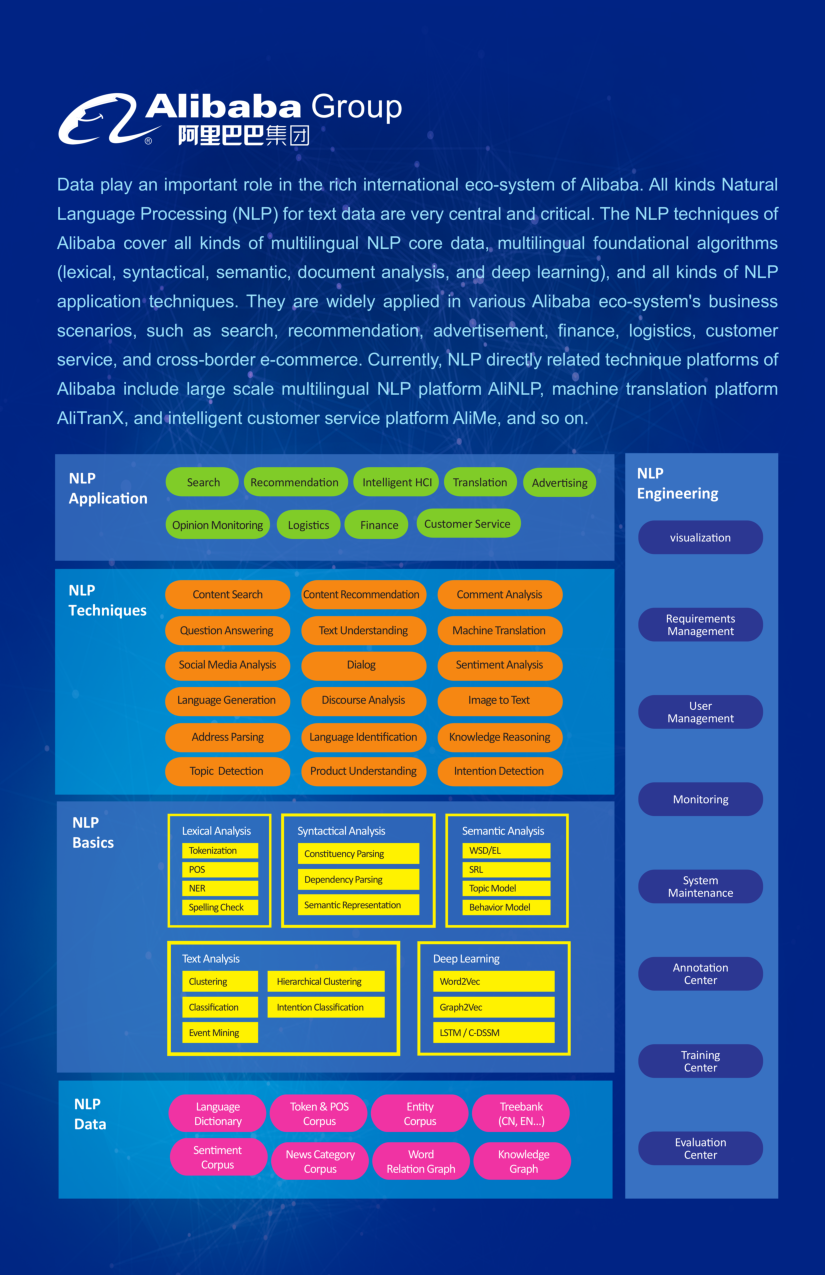
\includepdf[pages={1}]{content/ads/Platinum/01-Alibaba_resized}

\includepdf[pages={1}]{content/ads/Platinum/02-amazon_resized}

\includepdf[pages={1}]{content/ads/Platinum/03-Baidu_resized}
\includepdf[pages={1}]{content/ads/Platinum/04-Bloomberg_resized}
\includepdf[pages={1}]{content/ads/Platinum/05-Samsung_resized}

\includepdf[pages={1}]{content/ads/Platinum/06-Tencent_resized}

% Gold sponsors
\includepdfmerge[nup=1x2]{content/ads/Gold/01-eBay_resized, 1, content/ads/Gold/02-Elsevier_resized, 1}
\includepdfmerge[nup=1x2]{content/ads/Gold/03-KPMG_resized, 1, content/ads/Gold/04-Maluuba_resized, 1}
\includepdfmerge[nup=1x2]{content/ads/Gold/05-SAP_resized, 1, content/ads/Gold/06-IBM_resized, 1}
\includepdfmerge[nup=1x2]{content/ads/Gold/07-RIT_resized, 1, content/ads/Gold/08-NaverCorp_resized, 1}
\includepdfmerge[nup=1x2]{content/ads/Gold/09-NEC_resized, 1, content/ads/Gold/10-MSFT_resized, 1}

% Silver and Bronze sponsors
\includepdfmerge[nup=1x2]{content/ads/Silver/01-Adobe_resized+Gold, content/ads/Silver/02_03-Bosch+CVTE_resized}
\includepdfmerge[nup=2x2]{content/ads/Silver/04-duolingo_resized, content/ads/Silver/05-Huawei_resized, content/ads/Silver/06-Nuance_resized, content/ads/Silver/07-Sogou_resized}

\iftranslatorad
\includepdfmerge[nup=2x2]{content/ads/Silver/08-Oracle_resized, content/ads/Bronze/01-Grammarly_resized, content/ads/Bronze/02-Toutiao_resized, content/ads/Translator}
\else
\includepdfmerge[nup=2x2]{content/ads/Silver/08-Oracle_resized, content/ads/Bronze/01-Grammarly_resized, content/ads/Bronze/02-Toutiao_resized, content/ads/EmptyAd}
\fi

\else

% Platinum sponsors
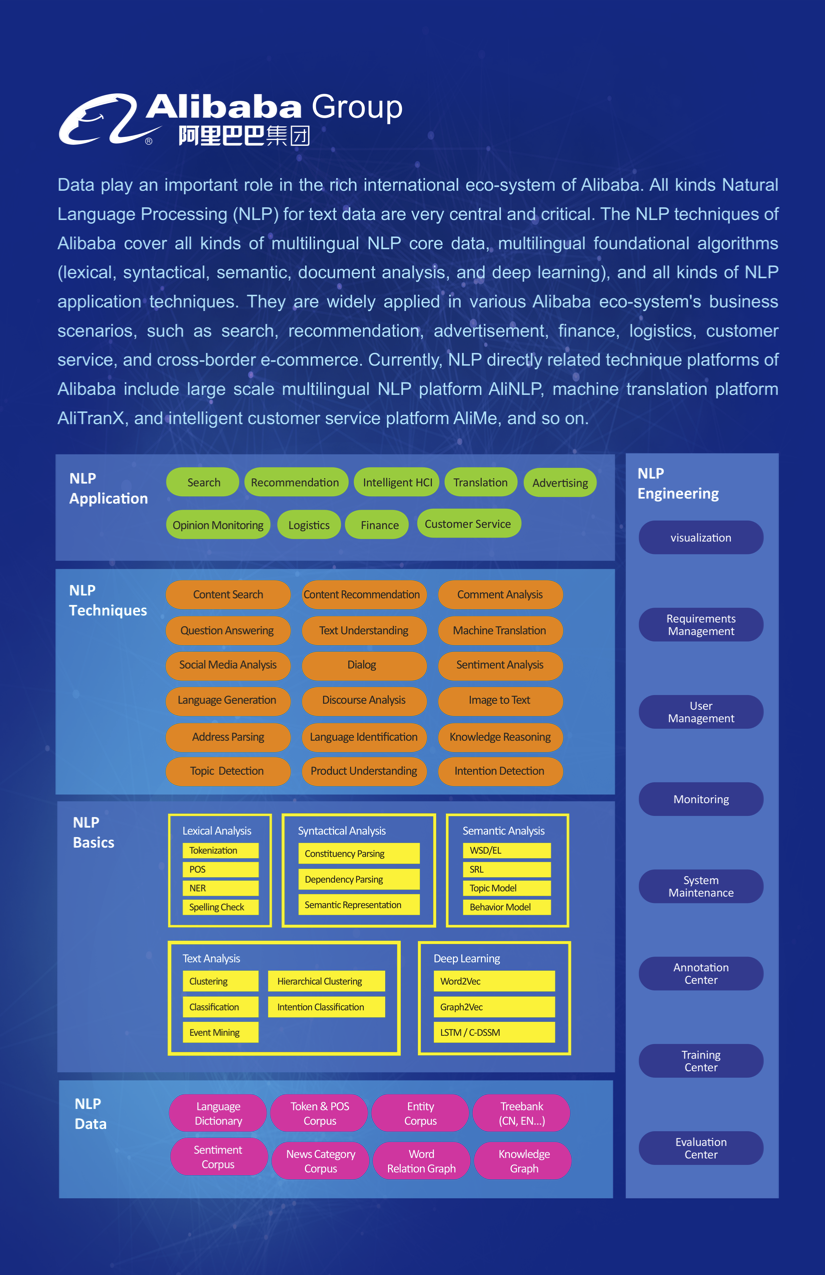
\includepdf[pages={1}]{content/ads/Platinum/01-Alibaba_resized_small.png}

\includepdf[pages={1}]{content/ads/Platinum/02-amazon_resized_small.png}

\includepdf[pages={1}]{content/ads/Platinum/03-Baidu_resized_small.png}

\includepdf[pages={1}]{content/ads/Platinum/04-Bloomberg_resized_small.png}
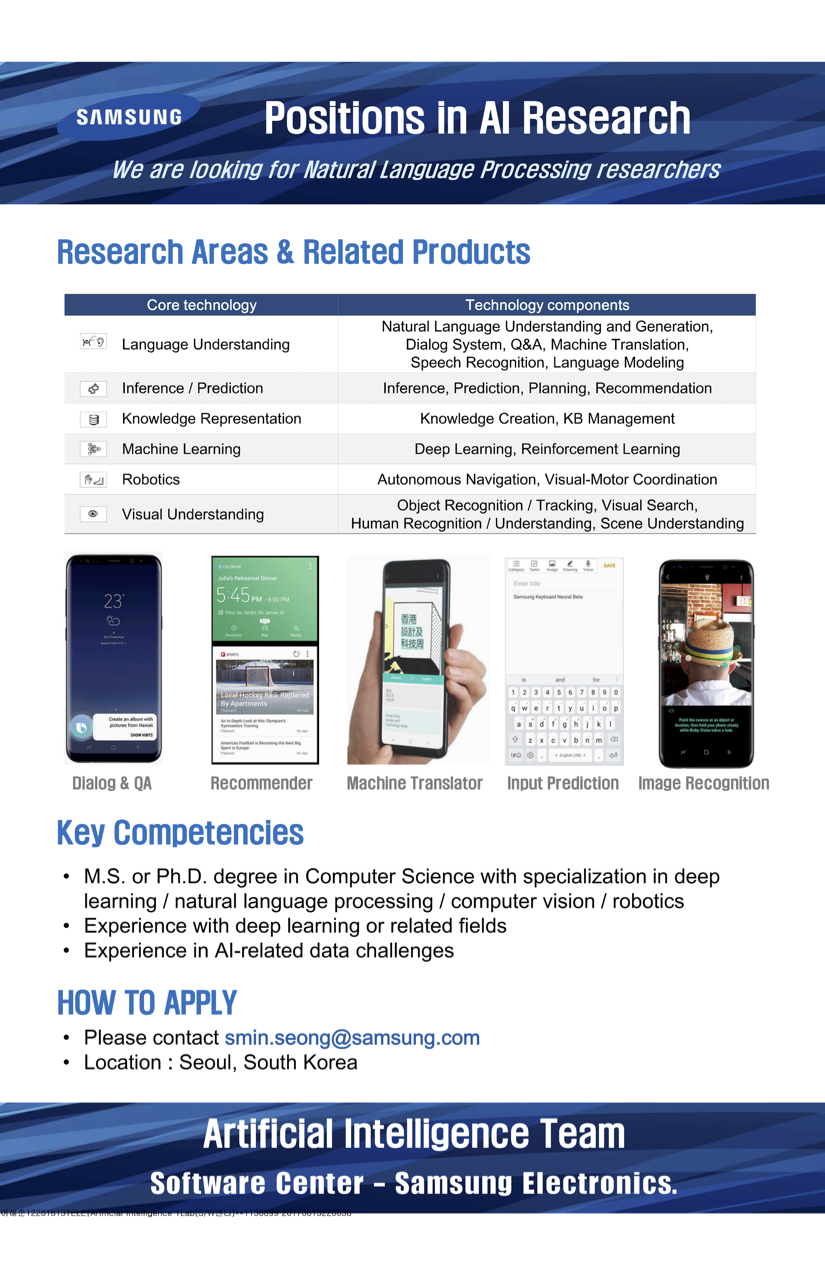
\includepdf[pages={1}]{content/ads/Platinum/05-Samsung_resized_small.png}

\includepdf[pages={1}]{content/ads/Platinum/06-Tencent_resized_small.png}

% Gold sponsors
\includepdfmerge[nup=1x2]{content/ads/Gold/01-eBay_resized_small.png, 1, content/ads/Gold/02-Elsevier_resized_small.png, 1}
\includepdfmerge[nup=1x2]{content/ads/Gold/03-KPMG_resized_small.png, 1, content/ads/Gold/04-Maluuba_resized_small.png, 1}
\includepdfmerge[nup=1x2]{content/ads/Gold/05-SAP_resized_small.png, 1, content/ads/Gold/06-IBM_resized_small.png, 1}
\includepdfmerge[nup=1x2]{content/ads/Gold/07-RIT_resized_small.png, 1, content/ads/Gold/08-NaverCorp_resized_small.png, 1}
\includepdfmerge[nup=1x2]{content/ads/Gold/09-NEC_resized_small.png, 1, content/ads/Gold/10-MSFT_resized_small.png, 1}

% Silver and Bronze sponsors
\includepdfmerge[nup=1x2]{content/ads/Silver/01-Adobe_resized+Gold_small.png, content/ads/Silver/02_03-Bosch+CVTE_resized_small.png}
\includepdfmerge[nup=2x2]{content/ads/Silver/04-duolingo_resized_small.png, content/ads/Silver/05-Huawei_resized_small.png, content/ads/Silver/06-Nuance_resized_small.png, content/ads/Silver/07-Sogou_resized_small.png}
\includepdfmerge[nup=2x2]{content/ads/Silver/08-Oracle_resized_small.png, content/ads/Bronze/01-Grammarly_resized_small.png, content/ads/Bronze/02-Toutiao_resized_small.png, content/ads/Translator}

\fi

\clearpage


%% BACK COVER %%%%%%%%%%%%%%%%%%%%%%%%%%%%%%%%%%%%%%%%%%%%%%%%%%%
\fancyfoot[C]{}
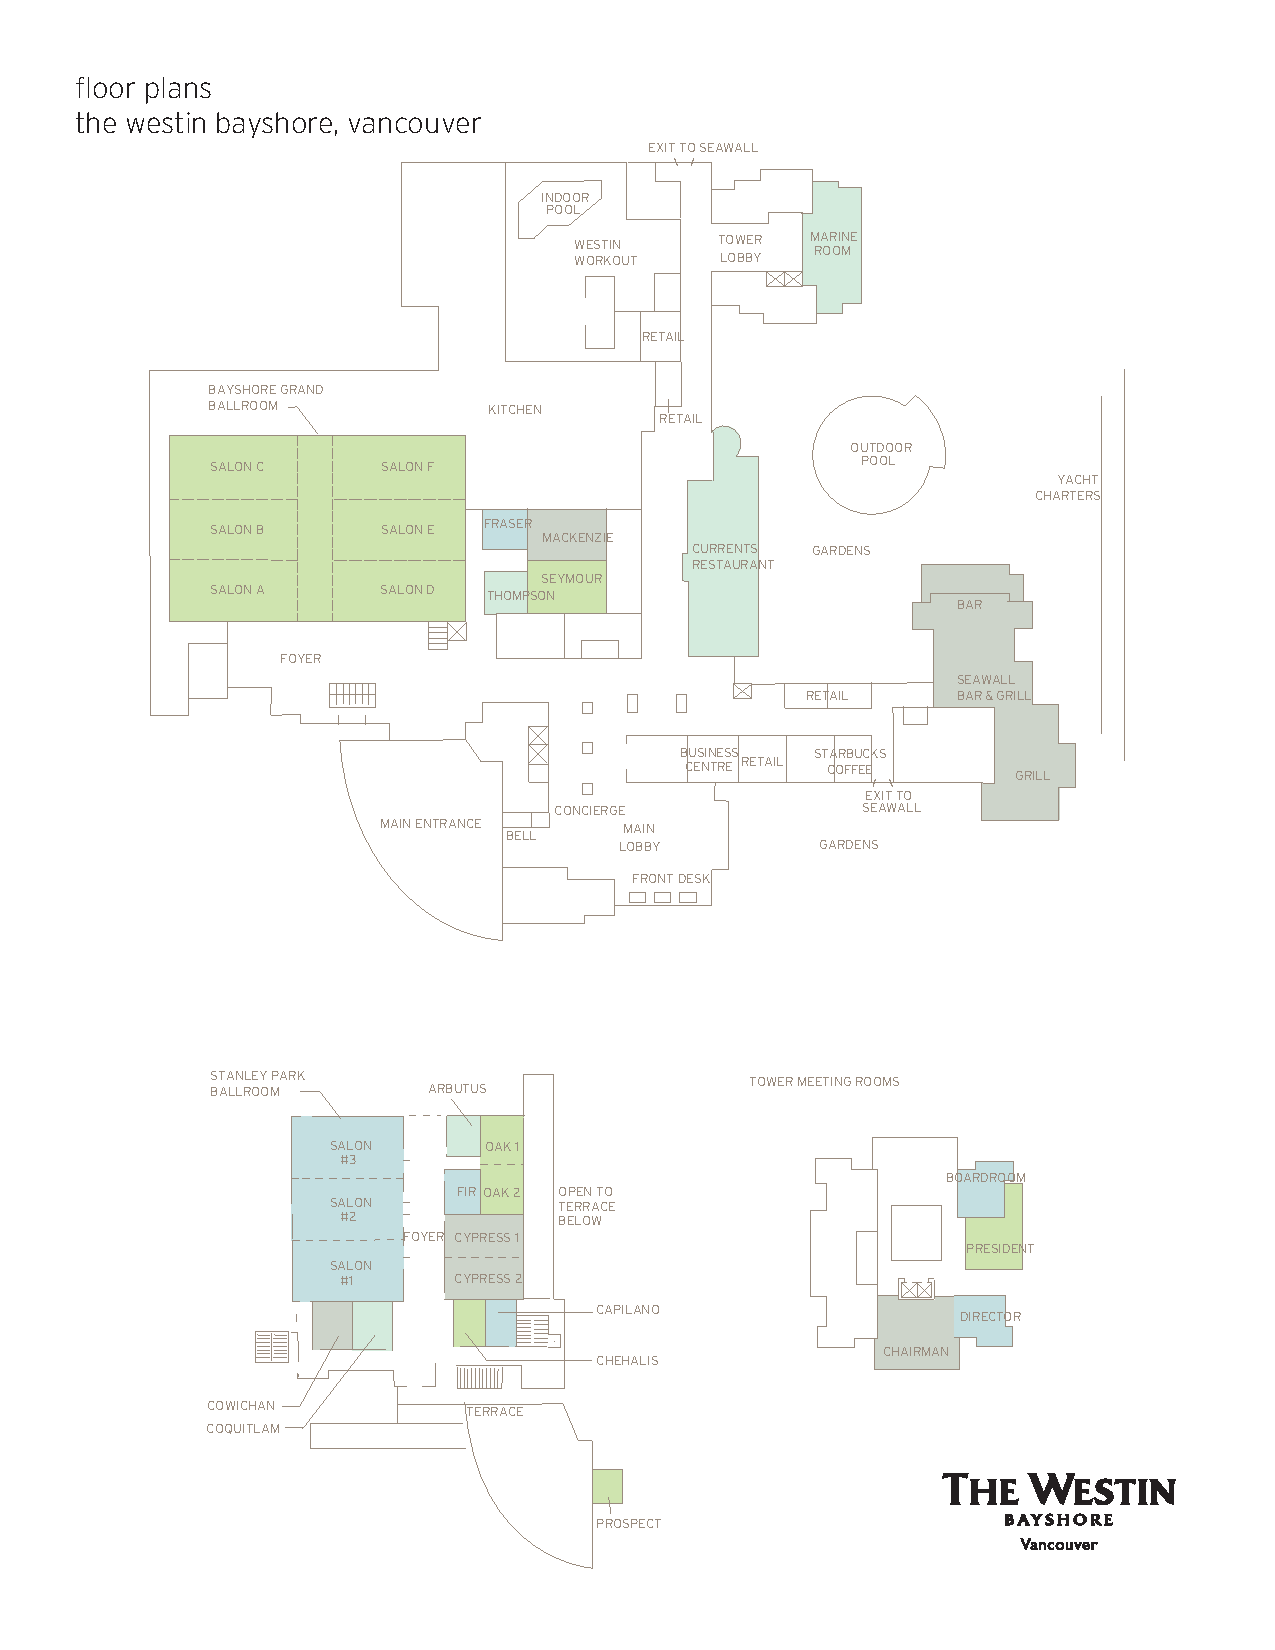
\includepdf[pages={1}]{content/fmatter/ACL17-westin-bayshore-floorplans}

\includepdf[pages={1}]{content/fmatter/back2.pdf}

\end{document}
